%%%%%%%%%%%%%%%%%%%%%%%%%%%%%%%%%%%%%%%%%
% Masters/Doctoral Thesis 
% LaTeX Template
% Version 2.5 (27/8/17)
%
% This template was downloaded from:
% http://www.LaTeXTemplates.com
%
% Version 2.x major modifications by:
% Vel (vel@latextemplates.com)
%
% This template is based on a template by:
% Steve Gunn (http://users.ecs.soton.ac.uk/srg/softwaretools/document/templates/)
% Sunil Patel (http://www.sunilpatel.co.uk/thesis-template/)
%
% Template license:
% CC BY-NC-SA 3.0 (http://creativecommons.org/licenses/by-nc-sa/3.0/)
%
%%%%%%%%%%%%%%%%%%%%%%%%%%%%%%%%%%%%%%%%%

%----------------------------------------------------------------------------------------
%	PACKAGES AND OTHER DOCUMENT CONFIGURATIONS
%----------------------------------------------------------------------------------------

\documentclass[
11pt, % The default document font size, options: 10pt, 11pt, 12pt
%oneside, % Two side (alternating margins) for binding by default, uncomment to switch to one side
english, % ngerman for German
singlespacing, % Single line spacing, alternatives: onehalfspacing or doublespacing
%draft, % Uncomment to enable draft mode (no pictures, no links, overfull hboxes indicated)
%nolistspacing, % If the document is onehalfspacing or doublespacing, uncomment this to set spacing in lists to single
%liststotoc, % Uncomment to add the list of figures/tables/etc to the table of contents
%toctotoc, % Uncomment to add the main table of contents to the table of contents
%parskip, % Uncomment to add space between paragraphs
%nohyperref, % Uncomment to not load the hyperref package
headsepline, % Uncomment to get a line under the header
%chapterinoneline, % Uncomment to place the chapter title next to the number on one line
%consistentlayout, % Uncomment to change the layout of the declaration, abstract and acknowledgements pages to match the default layout
]{MastersDoctoralThesis} % The class file specifying the document structure

\usepackage[utf8]{inputenc} % Required for inputting international characters
\usepackage[T1]{fontenc} % Output font encoding for international characters
\usepackage{mathpazo} % Use the Palatino font by default

\usepackage[backend=bibtex,style=numeric,natbib=true]{biblatex} % Use the bibtex backend with the authoryear citation style (which resembles APA)

\addbibresource{main.bib} % The filename of the bibliography
\usepackage[autostyle=true]{csquotes} % Required to generate language-dependent quotes in the bibliography
\usepackage{amssymb}  % to have some symbol I don't remember
\usepackage{multirow}
\usepackage{times} % to have tilde
\usepackage{textcomp} % to have tilde
\usepackage{amsmath} % to have math symbols, e.g. binom
\usepackage{mathtools}
\usepackage{slashed} % to have slashed

\newcommand{\beq}{\begin{equation}}
\newcommand{\eeq}{\end{equation}}
\newcommand{\cmsette}{$\sqrt{s}$ = 7 TeV}
\newcommand{\cmotto}{$\sqrt{s}$ = 8 TeV}
\newcommand{\stilde}{\tilde{s}}
\newcommand{\sbar}{\bar{s}}
\newcommand{\lagr}{\mathcal{L}}
\newcommand{\ifb}{fb$^{-1}$}
%----------------------------------------------------------------------------------------
%	MARGIN SETTINGS
%----------------------------------------------------------------------------------------

\geometry{
	paper=a4paper, % Change to letterpaper for US letter
	inner=2.5cm, % Inner margin
	outer=3.8cm, % Outer margin
	bindingoffset=.5cm, % Binding offset
	top=1.5cm, % Top margin
	bottom=1.5cm, % Bottom margin
	%showframe, % Uncomment to show how the type block is set on the page
}

%----------------------------------------------------------------------------------------
%	THESIS INFORMATION
%----------------------------------------------------------------------------------------

\thesistitle{Searches for supersymmetric particles in final states with multiple top and bottom quarks with the ATLAS detector} % Your thesis title, this is used in the title and abstract, print it elsewhere with \ttitle
\supervisor{Dr. Aurelio \textsc{Juste}} % Your supervisor's name, this is used in the title page, print it elsewhere with \supname
\examiner{} % Your examiner's name, this is not currently used anywhere in the template, print it elsewhere with \examname
\degree{Doctor of Philosophy} % Your degree name, this is used in the title page and abstract, print it elsewhere with \degreename
\author{Chiara \textsc{Rizzi}} % Your name, this is used in the title page and abstract, print it elsewhere with \authorname
\addresses{} % Your address, this is not currently used anywhere in the template, print it elsewhere with \addressname

\subject{Physics} % Your subject area, this is not currently used anywhere in the template, print it elsewhere with \subjectname
\keywords{} % Keywords for your thesis, this is not currently used anywhere in the template, print it elsewhere with \keywordnames
\university{\href{http://www.university.com}{UAB}} % Your university's name and URL, this is used in the title page and abstract, print it elsewhere with \univname
\department{\href{http://department.university.com}{Department of Physics}} % Your department's name and URL, this is used in the title page and abstract, print it elsewhere with \deptname
\group{\href{http://researchgroup.university.com}{IFAE}} % Your research group's name and URL, this is used in the title page, print it elsewhere with \groupname
\faculty{\href{http://faculty.university.com}{Physics}} % Your faculty's name and URL, this is used in the title page and abstract, print it elsewhere with \facname

\AtBeginDocument{
\hypersetup{pdftitle=\ttitle} % Set the PDF's title to your title
\hypersetup{pdfauthor=\authorname} % Set the PDF's author to your name
\hypersetup{pdfkeywords=\keywordnames} % Set the PDF's keywords to your keywords
}

\begin{document}

\frontmatter % Use roman page numbering style (i, ii, iii, iv...) for the pre-content pages

\pagestyle{plain} % Default to the plain heading style until the thesis style is called for the body content

%----------------------------------------------------------------------------------------
%	TITLE PAGE
%----------------------------------------------------------------------------------------

\begin{titlepage}
\begin{center}

% logos %%%%%%%%%%%%%%%%%%%%%%%%%%%%%%%%%%%%%%%%%%%%
\begin{figure}[h!]

\includegraphics[height=15mm]{figures/front/IFAE_logo-eps-converted-to.pdf}
\hfill

\includegraphics[height=15mm]{figures/front/uab_logo-eps-converted-to.pdf}
\end{figure}
 
% title %%%%%%%%%%%%%%%%%%%%%%%%%%%%%%%%%%%%%%%%%%%%
\vspace{0.5cm}
\HRule\\
\vspace{0.2cm}
{\huge \bf Searches for supersymmetric particles in final states with multiple top and bottom quarks with the ATLAS detector\\
\vspace{1cm}
Ph.D. dissertation}
\HRule\\
\par
\vspace{1.5in}
 
% author %%%%%%%%%%%%%%%%%%%%%%%%%%%%%%%%%%%%%%%%%%%
{\LARGE \bf Chiara Rizzi}
\vspace{0.3cm}
\par
Institut de F\'{i}sica d'Altes Energies\\
Universitat Aut\`{o}noma de Barcelona\\
Departament de F\'{i}sica\\
Facultat de Ci\`{e}ncies \\
Edifici Cn E-08193 Bellaterra (Barcelona)
\par
\vspace{0.5in}
 
 
% supervisor %%%%%%%%%%%%%%%%%%%%%%%%%%%%%%%%%%%%%%
\vfill
{\it Thesis director}\\
Aurelio Juste Rozas\\
ICREA / Institut de F\'{i}sica d'Altes Energies\\
Universitat Aut\`{o}noma de Barcelona\\
Edifici Cn E-08193 Bellaterra (Barcelona)

% tutor %%%%%%%%%%%%%%%%%%%%%%%%%%%%%%%%%%%%%%
\vfill
{\it Thesis tutor}\\
Maria Pilar Casado Lechuga\\
Universitat Aut\`{o}noma de Barcelona / Institut de F\'{i}sica d'Altes Energies\\
Universitat Aut\`{o}noma de Barcelona\\
Edifici Cn E-08193 Bellaterra (Barcelona)

\end{center}
\end{titlepage}

\sloppy
\titlepage
\cleardoublepage

%----------------------------------------------------------------------------------------
%	QUOTATION PAGE
%----------------------------------------------------------------------------------------

%\vspace*{0.2\textheight}
%\noindent\enquote{\itshape Thanks to my solid academic training, today I can write hundreds of words on virtually any topic without possessing a shred of information, which is how I got a good job in journalism.}\bigbreak
%\hfill Dave Barry

%----------------------------------------------------------------------------------------
%	ABSTRACT PAGE
%----------------------------------------------------------------------------------------

\begin{abstract}
\addchaptertocentry{\abstractname} % Add the abstract to the table of contents
This is the abstract of my awesome thesis. Test reference \cite{Reference1} \ldots
Other test \cite{Reference2}
\end{abstract}

%----------------------------------------------------------------------------------------
%	ACKNOWLEDGEMENTS
%----------------------------------------------------------------------------------------
%\begin{acknowledgements}
%\addchaptertocentry{\acknowledgementname} % Add the acknowledgements to the table of contents
%The acknowledgments and the people to thank go here, don't forget to include your project advisor\ldots
%\end{acknowledgements}

%----------------------------------------------------------------------------------------
%	LIST OF CONTENTS/FIGURES/TABLES PAGES
%----------------------------------------------------------------------------------------

\tableofcontents % Prints the main table of contents

%----------------------------------------------------------------------------------------
%	ABBREVIATIONS
%----------------------------------------------------------------------------------------

%\begin{abbreviations}{ll} % Include a list of abbreviations (a table of two columns)
%\textbf{LAH} & \textbf{L}ist \textbf{A}bbreviations \textbf{H}ere\\
%\textbf{WSF} & \textbf{W}hat (it) \textbf{S}tands \textbf{F}or\\
%\end{abbreviations}

%----------------------------------------------------------------------------------------
%	PHYSICAL CONSTANTS/OTHER DEFINITIONS
%----------------------------------------------------------------------------------------

%\begin{constants}{lr@{${}={}$}l} % The list of physical constants is a three column table
% The \SI{}{} command is provided by the siunitx package, see its documentation for instructions on how to use it
%Speed of Light & $c_{0}$ & \SI{2.99792458e8}{\meter\per\second} (exact)\\
%Constant Name & $Symbol$ & $Constant Value$ with units\\
%\end{constants}

%----------------------------------------------------------------------------------------
%	SYMBOLS
%----------------------------------------------------------------------------------------

%\begin{symbols}{lll} % Include a list of Symbols (a three column table)
%$a$ & distance & \si{\meter} \\
%$P$ & power & \si{\watt} (\si{\joule\per\second}) \\
%Symbol & Name & Unit \\
%\addlinespace % Gap to separate the Roman symbols from the Greek
%$\omega$ & angular frequency & \si{\radian} \\
%\end{symbols}

%----------------------------------------------------------------------------------------
%	DEDICATION
%----------------------------------------------------------------------------------------
%\dedicatory{For/Dedicated to/To my\ldots} 
%----------------------------------------------------------------------------------------
%	THESIS CONTENT - CHAPTERS
%----------------------------------------------------------------------------------------

\mainmatter % Begin numeric (1,2,3...) page numbering

\pagestyle{thesis} % Return the page headers back to the "thesis" style

% Include the chapters of the thesis as separate files from the Chapters folder
% Uncomment the lines as you write the chapters

%\chapter{Standard Model and Supersymmetry}
\label{chap:SMSUSY}

In this chapter we present first of all, in section \ref{sec:SM}, an overview of the Standard Model (SM), the theory used to describe elementary particles; in section \ref{SMlimits} we move to its main limits and in section \ref{sec:SUSY} we describe one of the most promising extension of the SM, Supersymmetry (SUSY), which is the theoretical framework in which the analysis presented in this thesis is set; current limits on the existence of SUSY particles will be presented. In this chapter and also in the rest of this thesis Natural units will be used, which means that the speed of light, $c$, and the Plank constant, $\hslash$, are normalized to unity and we thus use energy units to describe masses.

\section{Standard Model}
\label{sec:SM}

The Standard Model (SM) is the theory that nowadays best describes elementary particles (or at least the particles that at our present level of understanding we believe to be elementary) and the forces that act between them except from gravity. It has been formulated in the second half of the 20th century \cite{oerter:sm}, and in the last decades it has been tested to a high level of accuracy by many experiments. The predictions of this theory have led to the discovery of many particles and phenomena, like the top quark (discovered in 1995 by the $CDF$ and $D0$ collaborations \cite{cdf:top}, \cite{D0:top}), the tau neutrino (whose observation was announced in 2000 by the DONUT Collaboration \cite{kodama:taunu}), and last but not the least the Higgs boson, recently discovered by the ATLAS and CMS Collaborations at the Large Hadron Collider \cite{atlas:higgs}, \cite{cms:higgs}. 

In this section we will illustrate how particles and their interactions are described in the context of the SM, and how fields originally massless acquire mass through the interaction with the Higgs field.

%%%%%%%%%%%%%%%%%%%%%%%%%%%%%%%%%%%%%%%%%%

\subsection{Fundamental Particles and their Interactions}
\label{smint}
The SM is a gauge quantum field theory based on the group $SU(3) \times SU(2) \times U(1)$, which means that particles are described as excitations of quantum fields \cite{peskin:qft}.

The particles described by the SM and their mass, charge and spin properties are shown in Figure \ref{fig:SMpart}. The SM describes all fundamental forces in nature except from gravity; the interactions described by the SM and the properties of the corresponding gauge bosons are listed in table \ref{tab:sm_interazioni}, and will be further described in the next paragraphs. 
\begin{figure}
\begin{center}
%\includegraphics[width=0.6\textwidth]{./fig/particles.pdf}
\end{center}
\caption{Particles of the Standard Model and their mass, charge and spin properties}
\label{fig:SMpart}
\end{figure}

\begin{table}[h]
\centering
\begin{tabular}{llccc}
\hline
\multirow{2}*{Interaction} & \multirow{2}*{Carrier} & \multirow{2}*{$\frac{Q}{e}$} & \multirow{2}*{Mass [GeV]} & \multirow{2}*{\textbf{$\alpha$}} \\
 & & & &  \\
\hline
\hline
Strong & Gluons (g)  & 0 & 0 & 10 \\
\hline
Electromagnetic & Photon ($\gamma$) & 0 & 0  & $10^{-2}$ \\
\hline
\multirow{2}*{Weak} & $W^{+}$, $W^{-}$    &  +1, -1 &  	$80.385$ $\pm0.015$ GeV   & \multirow{2}*{$10^{-6}$}\\
 & $Z^{0}$  & 0 &  	$91.1876$ $\pm0.0021$ GeV &  \\
\hline
\end{tabular}
\caption[Interaction in the Standard Model]{Interaction in the Standard Model. Here the different force carriers are listed, with their electric charges and masses \cite{pdg:rev}; $\alpha$ is the coupling constant of the different interactions.}
\label{tab:sm_interazioni}
\end{table}

\subsubsection{Fermions}

Matter fields have spin $\frac{1}{2}$, and are called fermions, since they obey Fermi-Dirac statistic and satisfy Pauli exclusion principle: two identical fermions can not occupy the same quantum state simultaneously. Elementary fermions are further divided in two categories, based on the force they experience. Leptons are fermions that experience only the electroweak force, while quarks are fermions that are subject to both electroweak and strong force. Both leptons and quarks come into three generations of increasing mass. Leptons are observed as free particles, while quarks bind to form composite particles called hadrons, due to a particular property of the strong force that is called confinement. Hadrons are further classified into barions, which have spin $\frac{1}{2}$ and are built of three quarks, and mesons, which have integer spin and are built of 2 quarks. 

In quantum field theory, fermions are described through Dirac spinors, which are fields with four components, that incorporate both particle and antiparticle states. The kinematic of a fermionic field obeys the free Dirac lagrangian:
\beq
 \mathcal{L}_{free} = \bar{\psi} \left( i \gamma^{\mu} \partial_{\mu} - m \right) \psi
 \label{eq:ldirac}
\eeq

Where m is the mass of the fermion, $\gamma^{\mu}$ are the Dirac matrices, that obey anticommutation rules: $\left\lbrace \gamma^{\mu}, \gamma^{\nu}  \right\rbrace = 2 g^{\mu \nu} $, and $\partial_{\mu} $ is the four-vector derivative: $\partial_\mu = ({\partial / \partial t},\, \vec{\nabla})$. Using chirality operators, defined as:
\beq
P_L = (1 - \gamma_5)/2, \qquad\qquad
P_R = (1 + \gamma_5)/2
\eeq

one can project the left or right component of the field:

\beq
\psi_L = \frac{(1 - \gamma_5)}{2} \psi, \qquad\qquad
\psi_R = \frac{(1 + \gamma_5)}{2} \psi
\eeq

In the previous equations, $\gamma_5$ is defined as $\gamma_5 = i \gamma^0 \gamma^1 \gamma^2 \gamma^3 $, and it anticommutes with Dirac matrices:  $\left\lbrace \gamma^{\mu}, \gamma_{5}  \right\rbrace = 0$.

Using these relations one can show that, in the free Dirac lagrangian, the derivative keeps left and right terms separated, while the mass term couples them.



%Beside elementary fermions, described by the SM, there are also composite fermions, such as protons and neutrons, which are built of quarks.

\subsubsection{Bosons}

The SM also describes particles with integer spin, called bosons since they obey Bose-Einstein statistic. The force carriers are spin-1 particles, called gauge bosons. Beside gauge mediators, there is another boson predicted by the SM, the Higgs boson, which has spin 0; the other elementary particles acquire mass trough the interaction with the Higgs boson field as described in section \ref{sec:H}.

In quantum field theory, spin-0 fields obey the kinematics that derives from the free Klein-Gordon lagrangian, which if the field is real is:

\beq
\mathcal{L}_{free} = \frac{1}{2} \partial^\mu \phi \partial_\mu \phi + \frac{1}{2} m^2 \phi ^2 ,
\eeq
 
while for a complex scalar field is:
\beq
\mathcal{L}_{free} =  \partial^\mu \phi \partial_\mu \phi^* +  m^2 \phi \phi^* .
\eeq

On the other hand, a vector field $A^\mu$ with spin 1 obeys the Proca lagrangian if it has mass different from zero
\beq
\mathcal{L}_{free} =  - \frac{1}{4} F^{\mu \nu}F_{\mu \nu}+  \frac{1}{2} m^2 A^\mu A_\mu ,
\label{eq:lproca}
\eeq

and the Maxwell lagrangian if it has null mass

\beq
\mathcal{L}_{free} =  - \frac{1}{4} F^{\mu \nu}F_{\mu \nu} ,
\label{eq:lmax}
\eeq

where we have defined $F^{\mu \nu} = \partial^\mu A_\nu - \partial^\nu A_\mu$

\subsubsection{Gauge Symmetries}

The SM is a gauge theory, which means that interaction terms in the lagrangian are obtained by imposing that a theory which is invariant under a certain transformation retains its invariance also when the transformation becomes local (depends on the space-time coordinates). By invariance of a theory we mean that the lagrangian of the theory (or the action, which is the four-dimensional integral of the lagrangian) is unchanged after a certain transformation of the fields. The simplest example of gauge theory is Quantum Electrodynamics (QED), which will be later on incorporated in the theory of Electroweak Interactions. 

Let's consider Dirac free lagrangian in eq. \ref{eq:ldirac}. It is clearly invariant under the U(1) transformation $\psi \rightarrow e^{i \alpha} \psi$. If we move from a global to a local transformation ($\alpha \rightarrow \alpha (x) $), the theory keeps its invariance if we introduce:
\begin{itemize}
\item A vector field $A^\mu$, which transforms as $A^\mu \rightarrow A^\mu - \partial^\mu \alpha (x)$
\item A Maxwell lagrangian for the vector field like in eq. \ref{eq:lmax}
\item The covariant derivative $D^\mu = \partial^\mu + ieA^\mu$, that substitutes the regular derivative
\end{itemize}
By doing this the lagrangian of the theory becomes:
\beq
\mathcal{L} = \mathcal{L}^{Dirac} + \mathcal{L}^{Maxwell} + \mathcal{L}^{int} \quad \quad \quad \mathcal{L}^{int} = -e \bar{\psi} \gamma^{\mu} \psi A^\mu 
\label{eq:lqed}
\eeq

The term $\mathcal{L}^{int}$ in eq. \ref{eq:lqed} states the form of the allowed interactions between the fermionic field $\psi$ and $A^\mu$, the field of the photon. The only vertex allowed is the one with two fermion fields and one photon field. We can note that using the Proca lagrangian in eq. \ref{eq:lproca} instead of the massless version in eq. \ref{eq:lmax} would introduce a term $\frac{1}{2} m^2 A^\mu A_\mu$, which would not be invariant under gauge transformations, thus spoiling the gauge invariance of the theory.

In a more general gauge theory, the gauge transformation can be described as:
\beq
\psi \rightarrow e^{ig\theta_k \tau_k} \psi  
\eeq

Where $\theta_k = \theta_k(x)$ are space-time dependent functions and $\tau_k$ are the generators of the group and obey commutation relations: 
\beq
\left[ \tau_i, \tau_j \right] = i \epsilon_{ijk} \tau^k 
\eeq
In an Abelian gauge theory, like QED, this commutators are always zero. In a more general theory this is no longer true.

In this case we have to introduce
\begin{itemize}
\item A number of massless gauge fields $W^\mu_k$ equal to the number of generators of the group, that transform as $W^\mu_k \rightarrow W^\mu_k - \partial^\mu \theta_k - g \epsilon_{klm} \theta^m W^\mu_m $
\item A generalization of the covariant derivative of QED, $D^\mu = \partial^\mu + ig\tau^kW^\mu_k$
\item A free lagrangian for the vector fields with $F^{\mu \nu}_k = \partial_\mu W_k^\nu - \partial_\nu W_k^\mu - g \epsilon^k_lm W^\mu_l W^\nu_m$
\end{itemize}
In the last bullet, the tensor $F^{\mu,\nu}$ has a second order term due to the non-Abelian nature of the theory.

The SM is a gauge theory invariant under $SU(3)_C \times SU(2)_L \times U(1)_Y$, where $SU(3)_C$ is the color symmetry of strong interactions and $SU(2)_L \times U(1)_Y$ is the symmetry whose breaking brings to the electroweak interactions. These interactions are described in the next two sections.

\subsubsection{Electroweak Interaction}
The unified theory of electroweak interactions was first proposed by Glashow, Weinberg and Salam in the 1970's. It's a gauge theory based on the group $SU(2)_L \times U(1)_Y$, whose symmetry breaks at an energy scale of about 100 GeV, giving rise to the two interactions that we see at low energy: the electromagnetic interaction and the weak interaction, which can be further classified into weak charged currents (one with a positive and one with a negative charged mediator) and weak neutral currents. These four interactions require four different mediators, therefore the symmetry group of the electroweak theory must have four generators, which is true for the group $SU(2)_L \times U(1)_Y$. The gauge transformation is:
\beq
\psi \rightarrow e^{i \frac{g' \alpha_0}{2}Y} e^{ig \sum_k \alpha_k T^k} \psi ,
\label{eq:wint}
\eeq
where we have introduced T, the weak isospin operator (which is the SU(2) generator), and Y, the weak hypercharge operator. These two quantities are related to the electric charge Q through the relation:
\beq
Q = \frac{Y}{2} + T_3
\eeq
where $T_3$ is the third component of the weak isospin.
In eq. \ref{eq:wint} g is the weak isospin coupling strength, g' the weak hypercharge coupling strength. 

By introducing the covariant derivative we obtain:
\beq
\mathcal{L}_{int}^{EW} = -\frac{g'}{2} \left( \bar{\psi} \gamma_\mu Y \psi \right) B^\mu - g \sum_k \left( \bar{\psi} \gamma_\mu T^k \psi  \right) W_k^\mu
\eeq

Left-handed fields are isospin doublets with the same hypercharge, while right-handed fields are isospin singlets and therefore do not couple to the $W_k^\mu$ fields. When acting on an isospin doublet, the SU(2) generators are just $T^m= \frac{\sigma^m}{2}$, where $\sigma^m$ are the Pauli matrices:

\beq
	\sigma^1 = \left( \begin{array}{cc} 0 & 1 \\ 1 & 0 \end{array} \right) \qquad
	\sigma^2 = \left( \begin{array}{cc} 0 & -i \\ i & 0 \end{array} \right) \qquad
	\sigma^3 = \left( \begin{array}{cc} 1 & 0 \\ 0 & -1 \end{array} \right)
	\label{eq:paulimatrices}
\eeq

The gauge bosons $W_k^\mu$ and $B^\mu$ are the weak interaction eigenstates, which are different from the mass eigenstates, that are obtained by rotating $W_k^\mu$ and $B^\mu$ and requiring the photon field $A^\mu$ to have the correct quantum numbers. By doing this we obtain the physical fields, $W_\mu^\pm$, $A_\mu$, $Z_\mu$ as:

\beq
W_\mu^\pm = \frac{W_\mu^1 \mp W_\mu^2}{\sqrt{2}} \\
A_\mu = B_\mu \cos\theta_W + W^3_\mu \sin\theta_W  \\
Z_\mu = W^3_\mu \cos\theta_W - B_\mu \sin\theta_W
\label{eq:wein}
\eeq

The mixing angle is called Weinberg angle and its experimental value is $\sin^2\theta_W = 0.23113 \pm 0.0005 $. The coupling constants of the isospin and hypercharge are related to the electric charge:

\beq
e = \frac{gg'}{\sqrt{g^2 - g'^2}} \\
e = g \sin\theta_W = g' \cos\theta_W
\eeq

\subsubsection{Strong Interaction}
\label{sec:qcd}
The strong force is the force responsible for binding quarks into hadrons. The theory that describes strong interactions is Quantum Chromo-Dynamics (QCD), and the symmetry group of QCD is SU(3), which means that the transformation of the fields is:
\beq
\psi \rightarrow e^{i \alpha_c^a(x) t^a} \psi
\eeq

Unlike $SU(2)_L \times U(1)_Y$, which is a broken symmetry, $SU(3)_C$ is believed to be an exact symmetry of Nature, therefore the corresponding 8 gauge bosons (called gluons) are massless. Since the group is non-Abelian, the gluons carry color charge and interact not only with quarks but also among themselves. 
The renormalization of a gauge theory implies the definition of running coupling constants, which means that the coupling associated to the vertex of a certain theory is not fixed, but depends on the energy of the process. This is true for both QCD and QED, with the difference that while in QED the coupling constant increases with energy, in QCD it decreases, as shown in eq. \ref{eq:alfaQCD}:

\beq
\alpha(Q^2)=\frac{1}{b\log{\frac{Q^2}{\Lambda_{QCD}^2}}} \quad \quad b = \frac{11N_C-2n_f}{12\pi}
\label{eq:alfaQCD}
\eeq

$N_C$ is the number of colors and $n_f$ is the number of flavor of quarks.  $\Lambda_{QCD}$ represents the energy scale at which the perturbative QCD coupling diverges, and it's known to be around 250 MeV. In QCD $N_C=3$, which means that for $n_f<16$ the coupling constant of QCD shows a decreasing behaviour as the energy increases. This has some important consequences, that define the peculiarities of QCD:

\begin{itemize}
\item Perturbative QCD is valid only at high energies, as long as $\alpha(Q^2) << 1$
\item $\alpha(Q^2) \rightarrow 0$ as $Q^2 \rightarrow \infty $: when the momentum transferred in the interaction is big (which means at small distances), the coupling tends to zero. This behaviour is know as asymptotic freedom.
\item When the momentum transferred is small (large distances) the coupling is really strong, therefore it is not possible to extract quarks from hadrons. This is known as confinement. 
\item When we attempt to extract a quark from a hadron, it is more energetically favoured to create a new quark-antiquark pair. This is known as hadronization and is the reason of the formation of jets of hadrons.
\end{itemize}

%\subsubsection{Flavor Physics and CKM Matrix}


%%%%%%%%%%%%%%%%%%%%%%%%%%%%%%%%%%%%%%%%%%


\subsection{Higgs Physics}
\label{sec:H}

The Higgs boson was the last missing piece of the SM, and its observation in July 2012 is considered one of the milestones of experimental physics. In this section we will first describe how the Higgs mechanism, through spontaneous symmetry breaking, gives masses to elementary particles; then we will briefly present its discovery.

\subsubsection{Higgs Mechanism}

Among the gauge mediators of QED and weak interactions, only the photon is massless. The $W^\pm$ and the Z fields are massive. As we have discussed in section \ref{smint}, a mass term for the gauge bosons in the lagrangian would spoil the gauge invariance of the theory, and thus its renormalizability. For what concerns the fermions, a mass term would couple left-handed and right-handed fields: 

\beq
-m \bar \psi \psi = -m \bar \psi P_L^2 \psi - m \bar \psi P_R^2 \psi
	= -m \bar \psi_R \psi_L - m \bar \psi_L \psi_R
\eeq

We can overcome this problem by introducing a complex scalar field $\Phi$ with non vanishing vacuum expectation value (VEV). The lagrangian for this field is:

\beq
	\mathcal{L}_{\Phi} = ( \mathcal{D}_{\mu} \Phi)^{\dagger} (\mathcal{D}^{\mu} \Phi) - V(\Phi)  \quad \quad V(\Phi) = - \mu^2 \Phi^{\dagger} \Phi + \lambda (\Phi^{\dagger} \Phi)^2
	\label{eq:hpot}
\eeq

In the last equation $\mathcal{D}^{\mu}$ is the covariant derivative:

\beq
\mathcal{D}^{\mu} = \partial^{\mu} + i \frac{g'}{2} B^\mu Y + ig W^\mu_k T^k
\eeq

In the minimal model $\Phi$ is a weak isospin doublet with hypercharge Y=1 and isospin $T=\frac{1}{2}$, whose first component has electric charge Q=+1 and the second one is electrically neutral:

\beq
	\Phi = \left( \begin{array}{c} \phi^+  \\ \phi^0 \end{array} \right)
	= \frac{1}{\sqrt{2}} \left( \begin{array}{c} \phi_1 + i \phi_2 \\ \phi_3 + i \phi_4 \end{array} \right)
\eeq

In equation \ref{eq:hpot}, $\mu^2$ and $\lambda$ are real parameters, defining respectively the strength of the self-interaction of the field ant his mass term. Depending on the sign of these parameters we have different cases:

\begin{itemize}
\item If $\lambda$ is negative the potential V is unbounded from above, so it is not possible to have a stable vacuum state.
\item If $\lambda$ and $-\mu^2$ are both positive, V has a minimum at  $|\Phi| \equiv \sqrt{\Phi^{\dagger} \Phi} = 0$. Since in this case a gauge transformation acting on the vacuum would not change the vacuum, there would be no symmetry breaking.
\item If $\lambda$ is positive and $-\mu^2$ is negative, the minimum of the potential is displaced from zero, as shown in Figure \ref{fig:hpot}.
\end{itemize}

\begin{figure}
\begin{center}
%\includegraphics[width=0.7\textwidth]{fig/higgs_pot.jpg} 
\end{center}
\caption{Potential energy of the Higgs field. On the left panel we see the case where $\lambda$ and $-\mu^2$ are both positive; on the right panel there is the case in which $\lambda >0$ and $-\mu^2 < 0$, and the electroweak symmetry is broken.}
\label{fig:hpot}
\end{figure}

We thus require $\lambda > 0$ and $-\mu^2 < 0$. In this case we actually have a continuum of minima on the circumference of radius:
\beq
\sqrt{\Phi^{\dagger} \Phi} = \sqrt{ \frac{\mu^2}{2 \lambda} } = v
\eeq
The choice of one of these minima selects a vacuum state that is not invariant under a gauge transformation and the symmetry $SU(2)_L \times U(1)_Y$ is spontaneously broken. The $U(1)_Q$ symmetry should not be broken by the choice of the vacuum state. This means that we want $Q \Phi_0 = 0$, where $\Phi_0$ is the selected vacuum state, and this is achieved by setting $< \phi_1 > = 0$, $< \phi_2 > = 0$, $< \phi_4 > = 0$, $< \phi_3 > = v$, as shown in eq. \ref{eq:Qvacuum}

\beq
Q \Phi_0 = \left( \frac{Y}{2} + T_3 \right) \Phi_0 = \frac{1}{2} \left( 1 + \sigma_3 \right) \Phi_0 =  \left( \begin{array}{cc} 1 & 0 \\ 0 & 0 \end{array} \right) \left( \begin{array}{c} 0 \\ v \end{array} \right) = 0
\label{eq:Qvacuum}
\eeq

We can now expand $\Phi$ around its vacuum state:

\beq
	\Phi = \frac{1}{\sqrt{2}} \left( \begin{array}{c} 0 \\ v + \phi \end{array} \right)
\label{eq:hvphi}
\eeq

Here $\phi$ represents the physical field, since it is the displacement from the vacuum. By inserting this expansion in eq. \ref{eq:hpot} and substituting the electroweak gauge fields $W_k^\mu$, $B^\mu$ with the physical fields (with the rotation in eq. \ref{eq:wein}), one obtains the mass terms for the gauge fields $W^\pm$ and $Z$, the mass term for the Higgs field, the strength of the interaction of these fields with the Higgs and its self-interaction.
For what concerns the mass terms:
\beq
M_W^2 = \frac{g^2 v^2}{4}  \\
M_Z^2 = \frac{(g^2 + g^{\prime 2}) v^2}{4}
\eeq
while the field $A^\mu$ does not couple to the Higgs filed, therefore it does not acquire mass. The couplings of the other gauge fields with the Higgs boson are listed in Figure \ref{fig:hww} and \ref{fig:hzz}. We note that the couplings are proportional to the square of the mass of the gauge bosons.

\begin{figure}
\begin{center}
%\includegraphics[width=0.4\textwidth]{fig/2a.pdf} 
%\includegraphics[width=0.4\textwidth]{fig/2b.pdf}
\end{center}
\caption[eynman rules for the $hWW$ and $hhWW$ vertices]{Feynman rules for the $hWW$ and $hhWW$ vertices \cite{arxiv:higgs}.}
\label{fig:hww}
\end{figure}

\begin{figure}
\begin{center}
%\includegraphics[width=0.4\textwidth]{fig/3a.pdf} 
%\includegraphics[width=0.4\textwidth]{fig/3b.pdf}
\end{center}
\caption[Feynman rules for the $hZZ$ and $hhZZ$ vertices]{Feynman rules for the $hZZ$ and $hhZZ$ vertices \cite{martin:primer}.}
\label{fig:hzz}
\end{figure}

Introducing eq. \ref{eq:hvphi} in eq. \ref{eq:hpot} we find that the potential V can be expressed as:
\beq
V(\Phi) = \frac{\lambda}{4} \left( v + \phi \right)^4 - \frac{\mu^2}{2} \left( v + \phi \right)^2 = const + 2 \mu^2\phi^2 + 2 \sqrt{2}\frac{\mu}{\sqrt{\lambda}} \phi^3 + \lambda \phi^4
\eeq
Hence yielding a tree level Higgs mass of:
\beq
M_H = \sqrt{2} \mu
\eeq
And the self-couplings reported in Figure\ref{fig:hhh}.
\begin{figure}
\begin{center}
%\includegraphics[width=0.4\textwidth]{fig/5a.pdf} 
%\includegraphics[width=0.4\textwidth]{fig/5b.pdf}
\end{center}
\caption[Feynman rules for the $hhh$ and $hhhh$ vertices]{Feynman rules for the $hhh$ and $hhhh$ vertices \cite{martin:primer}.}
\label{fig:hhh}
\end{figure}

The mass terms for fermions are obtained introducing by hand a Yukawa coupling term between the fermionic fields and the Higgs field. Because of this, the coupling constant is a free parameter assumed to be proportional to the mass of the fermion, which is not constrained by the parameters of the theory, in contrast with the mass of the gauge bosons.
To give masses to up-type fermions through the mechanism of the spontaneous symmetry breaking, we need to introduce the complex conjugate of the Higgs doublet, given by:

\beq
 \Phi_C = i \sigma^2 \Phi^* 
	= i \left( \begin{array}{cc} 0 & -i \\ i & 0 \end{array} \right) 
	\left( \begin{array}{c} \phi^- \\ \phi^{0*} \end{array} \right)
	= \left( \begin{array}{c} \phi^{0*} \\ - \phi^- \end{array} \right)
\eeq

This way we can write the Yukawa term in the lagrangian as:
%\beq
%\mathcal{L}_{Yukawa} &=& - \left[  g_d \left( \bar{u}_L \,\, \bar{d}_L  \right) \Phi d_R +  g_u \left( \bar{u}_L \,\, \bar{d}_L  \right) \Phi_C u_R \right] + h.c. \\
%&=& - \frac{1}{\sqrt{2}} \left[  g_d \left( v + \phi \right) \bar{d}_L d_R + h.c. + g_u \left( v + \phi \right) \bar{u}_L d_u + h.c. \right] \nonumber
%\eeq

We now recognize the fermion mass terms:
\beq
M_{u,d} =  \frac{1}{\sqrt{2}} v g_{u,d}
\eeq

And the couplings to the Higgs boson, reported in Figure\ref{fig:hee}.

\begin{figure}
\begin{center}
%\includegraphics[width=0.4\textwidth]{fig/4.pdf} 
\end{center}
\caption[Feynman rules for the $hee$ vertex]{Feynman rules for the $hee$ vertex}
\label{fig:hee}
\end{figure}


\subsubsection{Discovery and Measurements of the Higgs Boson}

On July 4th 2012 the ATLAS and CMS experiments announced they had independently discovered a previously unknown boson, with properties compatible with those expected for the Higgs boson. The discovery was made using the data collected in 2011 ($\approx 5 fb^{-1}$ at \cmsette) and the first data of 2012 ($\approx 5 fb^{-1}$ at \cmotto), combining the results of two of the decay channels of the Higgs, $H \rightarrow \gamma \gamma $ and $H \rightarrow Z Z^* \rightarrow llll $, which are the channels where the invariant mass of the parent particle can be most easily reconstructed. 

Since 2012, measurements have been updated with the full \cmotto dataset ($\approx 20 fb^{-1}$, for a total of $\approx 25 fb^{-1}$). The invariant distributions of the decay products for these two channels is shown in Figure\ref{fig:hmass}, while in Figure \ref{fig:hsig} we see the Fit of $m_H$ and likelihood contours as a functions of the normalized signal yield $S= \frac{\sigma}{\sigma_{SM,mH = 125.36 \; GeV}}$ and $m_H$ for the individual $H \rightarrow \gamma \gamma $ and $H \rightarrow Z Z^* \rightarrow llll $ channels and their combination \cite{atlas:hmass}.

\begin{figure}[h]
\centering
%\includegraphics[width=.45\columnwidth]{./fig/hgammagamma.pdf}
%\includegraphics[width=.45\columnwidth]{./fig/h4l.pdf}
\caption[Invariant mass of the candidate Higgs boson in the $\gamma \gamma $ and 4-lepton channels]{(a) Invariant mass distribution in the $H \rightarrow \gamma \gamma $ analysis for data (7 TeV and 8 TeV samples combined). (b) Distribution of the four-lepton invariant mass for the selected candidates in the $m_{4l}$ range 80-170 GeV for the combined 7 TeV and 8 TeV data samples. Superimposed are the expected distributions of a SM Higgs boson signal for $m_H=124.5$ GeV normalized to the measured signal strength, as well as the expected $ZZ^*$ and reducible backgrounds \cite{atlas:hmass}. }
\label{fig:hmass}
\end{figure}

%\begin{figure}[h]
%\centering
%{\includegraphics[width=.45\columnwidth]{./fig/mh.pdf}} \quad
%{\includegraphics[width=.45\columnwidth]{./fig/signalstrenghth.pdf}} 
%\caption[Fit of $m_H$ and likelihood contours]{Results for the individual $H \rightarrow \gamma \gamma $ and $H \rightarrow Z Z^* \rightarrow llll $ channels and their combination. (a) Fit of $m_H$. (b) Likelihood contours as a functions of the normalized signal yield $S= \frac{\sigma}{\sigma_{SM,mH = 125.36 \; GeV}}$ and $m_H$  \cite{atlas:hmass}.}
%\label{fig:hsig}
%\end{figure}

The updated mass measurement is now:

\beq
\nonumber
m_H^{ATLAS} = 125.36 \pm 0.37(stat)\pm 0.18 (syst) \,\, GeV \\ \nonumber
m_H^{ATLAS} = 125.03 ^{+0.26}_{-0.27}(stat)^{+0.13}_{-0.15}  (syst) \,\, GeV 
\eeq

The observation of this new resonance now exploits also the channels $\tau \tau$ and $WW^* \rightarrow l \nu l \nu$, and the evidence is more than 7 $\sigma$. To prove that this new resonance is the Higgs boson, other properties beside its mass have to be tested. In particular, this resonance has spin-parity properties compatible with $J^P=0^+$, and $2^+$, $1^\pm$ and $0^-$ are disfavoured at more than 99\% CL.

%\clearpage

%%%%%%%%%%%%%%%%%%%%%%%%%%%%%%%%%%%%%%%%%%

\section{Limits of the Standard Model}
\label{SMlimits}

The SM is well verified at an high level of accuracy, but there are some hints that it might not be the fundamental theory that describes Nature. In this section we will describe some of these characteristics, with particular emphasis on those solved by Supersymmetry.

\subsubsection*{Neutrino Masses}
The SM predicts neutrinos with null mass, while experimental observation of neutrino oscillations proves that neutrinos have mass different from zero.

\subsubsection*{Hierarchy Problem}
In section \ref{sec:H} we obtained the Higgs mass term, but that was only the tree level approximation. The correct calculation of the Higgs mass should include radiative corrections to the Higgs propagator coming from loops of all the other particles coupling to the Higgs boson. In particular, for fermions the coupling with the Higgs is given by a Yukawa term, $-\lambda_f \phi \bar{f} f$. The loop integrals originating from these corrections are divergent, and the regularization of the theory requires a cut-off; since we know that at the Plank scale, $10^{19}$ GeV, the SM is not anymore valid, e reasonable cut-off for the momentum of the particles in the loop is the Plank scale itself; at an higher energy scale, new physics beyond the SM must enter the theory. The contribution to the Higgs mass given by a loop of fermions as the one shown in figure \ref{fig:hcorr}(a) is given by:

\beq
\Delta m_H^2 \>=\>  
-{|\lambda_f|^2\over 8 \pi^2} \Lambda_{cut-off}^2 + \ldots
\label{eq:divhf}
\eeq

where the ellipses are meant to represent the other terms logarithmic in $\Lambda_{cut-off}$. The corrections to the mass are thus of the same order of magnitude of the cut-off scale. To yield a Higgs mass of about 125 GeV, these corrections from radiative terms should cancel out with the bare Higgs mass term. This requires a fine tuning of the parameters, which should be of the order of $\frac{m_H}{\Lambda} \approx 10^{-17}$. 

All the fermions of the SM contribute to the correction to the Higgs propagator. However, since the couplings of fermions to the Higgs boson (and thus their contribution to the radiative corrections to the propagator) are proportional to their masses, the largest correction is given by the loop of the top quark.

A possible solution could be to choose a cut-off scale not too large, but in that case one should have new physics entering the theory at that scale. On the other hand, if we consider a massive scalar particle S, for dimensional arguments its coupling to the Higgs boson should be of the form $ -\lambda_S
|\phi|^2 |S|^2$. In this case the correction to the propagator, shown in figure \ref{fig:hcorr}(b), is given by:
 
\beq
\Delta m_H^2 \>=\> {\lambda_S\over 16 \pi^2}
\left [\Lambda_{cut-off}^2 - 2 m_S^2
\> {\rm ln}(\Lambda_{cut-off}/m_S) + \ldots
\right ].
\label{eq:divhs}
\eeq 
 
We note that in the two equations \ref{eq:divhf} and \ref{eq:divhs}, the corrections to the squared mass have opposite sign. If we imagine to associate to each fermion of the SM two complex scalars such that $\lambda_S = |\lambda_f|^2$, the two contributions would cancel each other. As we will see in the next sections, this is what is postulated by Supersymmetry (SUSY). 

\begin{figure}
\begin{center}
%%\includegraphics[width=0.7\textwidth]{fig/higgs_corr.pdf} 
\end{center}
\caption[Loop corrections to the Higgs boson propagator]{Loop corrections to the Higgs boson propagator, coming from a fermion (a) and a scalar (b)}
\label{fig:hcorr}
\end{figure}

\subsubsection*{Unification of coupling constants}

As we have discussed in section \ref{sec:qcd}, the QCD coupling constant decreases with energy, while the $U(1)_Y$ and $SU(2)_L$ couplings have the opposite behaviour. If the SM were the low energy limit of a simpler gauge theory, with only one coupling constant, the values of the three different coupling constants of the SM should converge at high energy in one single point, as predicted by grand unification theories. The renormalization group equations in the SM are such that there is no energy scale at which this happens. In SUSY theories the particle content is different, and in some models, like the Minimal Supersymmetric Standard Model (MSSM), this unification can take place, as shown in figure \ref{fig:couplings}.

\begin{figure}
\begin{center}
%\includegraphics[width=0.45\textwidth]{fig/unification_couplings.pdf} 
\end{center}
\caption[Evolution of the coupling constants]{Evolution of the inverse of the gauge couplings in the SM (dashed lines) and in the Minimal Supersymmetric Standard Model, one of the SUSY models. In the SUSY scenario the convergence if the couplings to a single value at high energies is better than in the SM.}
\label{fig:couplings}
\end{figure}

\subsubsection*{Dark Matter and Dark Energy}
The SM describes only ordinary matter, which is made of fermions and hadrons. From cosmological results, we now that ordinary matter accounts only for the 4\% of the content of the universe. First of all, not all the matter behaves like ordinary matter. The rotational velocity of the galaxies does not decrease with the distance from the center of the galaxies as it should if the content of matter was in a one to one correspondence with the light we see; this implies that there is another kind of matter, that is subject to gravitational force but does not shine. This kind of matter is called dark matter, and accounts for another 22\% of the energy content of the universe. The remaining 76\% it thought to be dark energy, which is responsible for the accelerated expansion of the universe.

Supersymmetric theories that are R-parity conserving (described in section \ref{sec:rpar}), supply a good candidate for dark matter, the Lightest Supersymmetric Partner (LSP). Nowadays there is not a field theory able to propose a good candidate for dark energy.


\subsubsection*{Barionic Asimmetry of the Universe}
In the context of the SM, the CKM matrix with its complex phase offers a source of CP asymmetry. This is however not enough to explain the asymmetry between the content of matter and anti-matter that we observe in our universe.

\subsubsection*{Charge Quantization}
While the quantization of the angular momentum is explained by the non-Abelian nature of the SU(2) group, the symmetry group of QED, U(1), is Abelian, and so it does not require the conserved quantity (the electric charge) to be quantized. 

Also the choice of the hypercharge Y is arbitrary, and it is assigned so that the electron charge and the proton charge, which in principle should be two independent parameters of the SM, have the same absolute value.

\subsubsection*{Gravity}
The SM describes only three of the four fundamental forces (electromagnetic, weak and strong), while gravity is not included in this theory. This is a conceptual problem, but it also limits the validity of the theory to the scale at which gravity effects become comparable to the effects of the other forces acting between elementary particles; this is known as Plank scale, and it is about $10^{19}$ GeV. 

\subsubsection*{Free Parameters}
The free parameters of the SM are:
\begin{itemize}
\item 9 fermion masses (+ 3 if $m_\nu$ is different from zero)
\item 3 angles and 1 phase for the CKM matrix (+ 3 + 1 if $m_\nu$ is different from zero)
\item 3 coupling constants for U(1), SU(2), SU(3)
\item 1 for the Higgs mass and 1 for the Z mass (the masses of the other gauge bosons can be obtained form these)
\end{itemize}
So we have 18 free parameters, which become 25 if we include neutrino masses. This large number of free parameters is seen as a hint of the SM not being a fundamental theory.


%%%%%%%%%%%%%%%%%%%%%%%%%%%%%%%%%%%%%%%%%%
%%%%%%%%%%%%%%%%%%%%%%%%%%%%%%%%%%%%%%%%%%
%%%%%%%%%%%%%%%%%%%%%%%%%%%%%%%%%%%%%%%%%%

\section{Supersymmetry}
\label{sec:SUSY}

Supersymmetry (SUSY) is one of the most attractive extensions of the SM \cite{martin:primer}. In this section an introduction to SUSY will be given. Then we will take a look at the simplest SUSY model, Wess-Zumino model, and techniques used to include interactions in it.

%%%%%%%%%%%%%%%%%%%%%%%%%%%%%%%%%%%%%%%%%%

\subsection{Introduction}
\label{sec:susyintro}

A supersymmetry transformation rotates a bosonic state into a fermionic state and vice-versa. The operator that generates this transformation is Q, the supercharge:

\beq
Q |{\rm Boson}\rangle = |{\rm Fermion }\rangle \qquad\qquad
Q |{\rm Fermion}\rangle = |{\rm Boson }\rangle .
\eeq

Since Q interchanges bosonic and fermionic states, it must carry a fermionic index. $Q^\dagger$, the hermitian conjugate of Q, is also a symmetry generator. The spinorial nature of the  supercharge operator seems to be in contrast with Coleman-Mandula theorem, that states that ``space-time and internal symmetries cannot be combined in any but a trivial way'' \cite{coleman:mandula}; this implies that the generators of the internal transformations should be scalar. 
This problem was solved by the Haag-Lopuszanski-Sohnius extension of the theorem, that allows such fermionic generators and puts restrictions on the algebra of commutation and anticommutation relations they must satisfy, called supersymmetry algebra:

%\beq
%&&\{ Q, Q^\dagger \} = P^\mu , \label{eq:susyalgone}
%\\
%&&\{ Q,Q \} = \{ Q^\dagger , Q^\dagger \} = 0 , \label{eq:susyalgtwo}
%\\
%&&[ P^\mu , Q  ] = [P^\mu, Q^\dagger ] = 0 ,\label{eq:susyalgthree}
%\eeq

where $P^\mu$ is the four-momentum operator, the generator of space-time translations. Equation \ref{eq:susyalgone} states that by applying a combination of the supercharge operator and its hermitian conjugate one can obtain a translation in space-time.


The irreducible representations of the supersymmetry algebra (the particles predicted by the theory) are classified into supermultiplets, that include SM particles and the particles that SUSY associates them, called superpartners. Equation \ref{eq:susyalgthree} implies that $[ (P^\mu)^2 , Q  ]=0$, so all particles inside the same supermultiplet should have the same mass. It can also be sown that, within a single supermultiplet, the number of fermionic degrees of freedom has to be equal to the number of bosonic degrees of freedom. This gives us a guideline to construct and classify supermultiplets:

\begin{description}

\item[Chiral supermultiplet] If we consider a Weyl fermion, it has two helicity states and so two degrees of freedom; it then needs to be matched with two real scalar fields which, since a Weyl fermion is a complex object, are naturally merged into a single complex field. The superpartner of a fermion is called sfermion (it stands for scalar-fermion), so we have that the superpartner of the electron is called selectron, the superpartner of the top quark is called stop and so on. From the graphical point of view, superpartners are indicated with the same letter identifying the SM particles, but with a $\texttildelow$ on top of it. For example the superpartner of the $e_L$ is the $\tilde{e}_L$. We notice that, in the case of sfermions, the L,R subscript looses its meaning of helicity (sfermions are scalars) and it only refers to helicity of the SM partner. The Higgs sector of SUSY gives rise to two chiral supermultiplets as well.

\item[Gauge supermultiplet] Gauge bosons are spin 1 particles and, before symmetry breaking, they are massless. A massless spin 1 particle has 2 bosonic degrees of freedom, which means it has to be associated with a spin $\frac{1}{2}$ Weyl fermion; these fermions have the same name of the SM particles but with a -ino suffix (gauginos). Since gauge bosons belong to the adjoined representation of the gauge group (which is its own conjugate), left-handed and right-handed gauginos must have the same gauge transformation. 

\item[Gravitational supermultiplet] If we want a theory that includes gravity, we have to postulate the existence of a massless spin 2 graviton. Its superpartner, the gravitino, has to be a spin $\frac{3}{2}$ particle.

\end{description}

The chiral multiplets of a minimal supersymmetric extension of the SM, their spin and properties under gauge transformations are reported in table \ref{tab:chiral}, while the gauge multiplets are reported in table \ref{tab:gauge}. We have to notice that these particles do not have to be mass eigenstates, since there can be mixing between the electroweak gauginos and higgsinos, and between the sfermions associated with the left-handed or right-handed component of a SM particle. The only SUSY particles that do not mix are gluinos, since they do not have the correct quantum numbers to mix with other particles.

It is worth noticing that, in table \ref{tab:chiral}, the Higgs sector is more extended than one could think. It seems natural that the Higgs boson, being a spin-0 particle, has to be part of a chiral supermultiplet. But the minimum content of Higgs supermultiplets in SUSY is two. There are different arguments to prove this, one of them being the need to avoid introducing a gauge anomaly in the theory. In order for the gauge anomalies to cancel, we need to have $\sum Tr \left[Y^3  \right]$, where Y is the hypercharge and the sum runs over all the left-handed fermions of the theory; this condition is satisfied in the SM. If we introduce only one Higgs supermultiplet, the superpartner of the Higgs would be a weak isospin doublet with $Y=\frac{1}{2}$ or $Y=-\frac{1}{2}$. In both cases, the new fermion would spoil the cancellation of anomalies. This can be avoided by introducing two Higgs sumpermultiplets, one with $Y=\frac{1}{2}$ and one with $Y=-\frac{1}{2}$.

\renewcommand{\arraystretch}{1.4}
\begin{table}[tb]
\begin{center}
\begin{tabular}{c c c c c}
\hline
\multicolumn{2}{c}{Names} 
& spin 0 & spin 1/2 & $SU(3)_C ,\, SU(2)_L ,\, U(1)_Y$
\\  \hline\hline
squarks, quarks & $Q$ & $({\stilde u}_L\>\>\>{\stilde d}_L )$&
 $(u_L\>\>\>d_L)$ & $(\>{\bf 3},\>{\bf 2}\>,\>{1\over 6})$
\\
($\times 3$ families) & $\sbar u$
&${\stilde u}^*_R$ & $u^\dagger_R$ & 
$(\>{\bf \overline 3},\> {\bf 1},\> -{2\over 3})$
\\ & $\sbar d$ &${\stilde d}^*_R$ & $d^\dagger_R$ & 
$(\>{\bf \overline 3},\> {\bf 1},\> {1\over 3})$
\\  \hline
sleptons, leptons & $L$ &$({\stilde \nu}\>\>{\stilde e}_L )$&
 $(\nu\>\>\>e_L)$ & $(\>{\bf 1},\>{\bf 2}\>,\>-{1\over 2})$
\\
($\times 3$ families) & $\sbar e$
&${\stilde e}^*_R$ & $e^\dagger_R$ & $(\>{\bf 1},\> {\bf 1},\>1)$
\\  \hline
Higgs, higgsinos &$H_u$ &$(H_u^+\>\>\>H_u^0 )$&
$(\stilde H_u^+ \>\>\> \stilde H_u^0)$& 
$(\>{\bf 1},\>{\bf 2}\>,\>+{1\over 2})$
\\ &$H_d$ & $(H_d^0 \>\>\> H_d^-)$ & $(\stilde H_d^0 \>\>\> \stilde H_d^-)$& 
$(\>{\bf 1},\>{\bf 2}\>,\>-{1\over 2})$
\\  \hline
\end{tabular}
\caption{Chiral supermultiplets in the Minimal Supersymmetric Standard Model.
The spin-$0$ fields are complex scalars, and the spin-$1/2$ fields are 
left-handed two-component Weyl fermions.\label{tab:chiral}}
\vspace{-0.6cm}
\end{center}
\end{table}


\renewcommand{\arraystretch}{1.55}
\begin{table}[t]
\begin{center}
\begin{tabular}{c c c c}
\hline
Names & spin 1/2 & spin 1 & $SU(3)_C, \> SU(2)_L,\> U(1)_Y$\\
\hline\hline
gluino, gluon &$ \stilde g$& $g$ & $(\>{\bf 8},\>{\bf 1}\>,\> 0)$
\\
\hline
winos, $W$ bosons & $ \stilde W^\pm\>\>\> \stilde W^0 $&
 $W^\pm\>\>\> W^0$ & $(\>{\bf 1},\>{\bf 3}\>,\> 0)$
\\
\hline
bino, B boson &$\stilde B^0$&
 $B^0$ & $(\>{\bf 1},\>{\bf 1}\>,\> 0)$
\\
\hline
\end{tabular}
\caption{Gauge supermultiplets in
the Minimal Supersymmetric Standard Model.\label{tab:gauge}}
\vspace{-0.45cm}
\end{center}
\end{table}

%%%%%%%%%%%%%%%%%%%%%%%%%%%%%%%%%%%%%%%%%%
%%%%%%%%%%%%%%%%%%%%%%%%%%%%%%%%%%%%%%%%%%

\subsection{Supersymmetric Lagrangians and Super-Multiplets}

In this section we give an overview of the simplest SUSY model and how SUSY-invariant interactions are included into it.

\subsubsection*{Wess-Zumino Model}

We want now to build the simplhiggsest supersymmetric model, called Wess-Zumino model, starting from a theory that contains only a left-handed Weyl spinor $\psi$ and a complex scalar field $\phi$. The free lagrangian for this theory is:

\beq
\mathcal{L}_{WZ} = \partial^\mu \phi^* \partial_\mu \phi + i \psi^\dagger \bar{\sigma}^\mu \partial_\mu \psi
\label{eq:WZL}
\eeq

This is the massless, non interacting Wess-Zumino lagrangian. The corresponding action, which is the four-dimensional integral of the lagrangian, is:

\beq
S_{WZ} = \int d^4x \; \mathcal{L}_{WZ}
\eeq

We now introduce an infinitesimal parameter $\epsilon$ with a fermionic index: 
%$\epsilon \equiv \binom{\epsilon^1}{\epsilon^2}$, 
% chiara: decomment
that does not depend on the space-time coordinates (global symmetry). We define an infinitesimal transformation of both the scalar and the chiral fields:

\beq
\delta \phi = \epsilon^\dagger \psi \qquad ;  \qquad \delta \psi = -i(\sigma^\nu \epsilon)\partial_\nu \phi 
\delta \phi^* = \psi^\dagger \epsilon \qquad  ; \qquad \delta \psi^\dagger = i(\epsilon^\dagger \sigma^\nu )\partial_\nu \phi^*
\eeq

It can be shown that the Wess-Zumino action is invariant under these transformations, that constitute then a symmetry of the system (Supersymmetry). The field $\binom{\phi}{\psi}$  is a supermultiplet.

%%%%%%%%%%%%%%%%%%%%%%%%%%%%%%%%%%%%%%%%%%

\subsubsection*{Chiral Super-Multiplets}

The Wess-Zumino lagrangian as in eq. \ref{eq:WZL} does not provide a particularly interesting model, since it does not include interactions. In order to introduce interactions in the theory, we write the most general potential which is invariant under SUSY transformations and is renormalizable. The lagrangian has the form:

%\beq
% \begin{split}
%  \mathcal{L}_{chiral}^{int} &= -\frac{1}{2} \left( W^{i,j} \psi_i \psi_j + W^*_{i,j} \psi^{ \dagger i}  \psi^{ \dagger j} \right) + W^i W^*_i = \\
%  								& =  -\frac{1}{2} \left( M^{i,j} \psi_i \psi_j + M^*_{i,j} \psi^{ \dagger i}  \psi^{ \dagger j} \right) + M^{ij} M^*_{ik} \phi_j \phi^{* k} + \\
%  								& -\frac{1}{2} \left( y^{ijk} \psi_i \psi_j \phi_k + y^*_{ijk} \psi^{\dagger i} \psi^{\dagger j} \phi^{* k} \right) + \\
%  								& + \frac{1}{2} \left(  M^{ij} y^*_{ikl} \phi_j \phi^{*k} \phi^{*l}      +    M^*_{ij} y^{ikl} \phi_k \phi_l \phi^{*j}    \right) + \\			& +\frac{1}{4} y^{ijk} y^*_{ilm} \phi_j \phi_k \phi^{*l} \phi^{*m} ,
%\end{split}
%\label{eq:lint}
%\eeq

where we have introduced the Superpotential:

\beq
W =
{1\over 2} M^{ij} \phi_i \phi_j + {1\over 6} y^{ijk} \phi_i \phi_j \phi_k,
\label{superpotential}
\eeq

and its derivatives:

\beq
W^i \equiv \frac{\partial W}{\partial \phi_i} = M^{ij} \phi_j + \frac{1}{2} y^{ijk} \phi_j \phi_k 
\\
W^{ij} = {\delta^2 \over \delta\phi_i\delta\phi_j} W = M^{ij} + y^{ijk} \phi_k
\eeq

The Superpotential has to be a holomorfic function of the chiral superfields; this will play an important role in the definition of the Higgs sector of the MSSM. In equ. \ref{eq:lint} we have used the notation:

\beq
\psi_i \psi_j = \psi_i^T \begin{pmatrix}
0 & -1 \\ 1 & 0
\end{pmatrix} \psi_j
\\
\psi^{\dagger i} \psi^{\dagger j} \equiv \left(  \psi^i \psi^j   \right)^*
\eeq

The overall chiral lagrangian becomes:

\beq
 \begin{split}
  \mathcal{L}_{chiral} &=  \partial^\mu \phi^{* i} \partial_\mu \phi_i  M^{ij} M^*_{ik} \phi_j \phi^{* k} +    \; \; \;  massive \, scalars\\
&  + i \psi^{\dagger i} \bar{\sigma}^\mu \partial_\mu \psi_i + -\frac{1}{2} \left( M^{i,j} \psi_i \psi_j + M^*_{i,j} \psi^{ \dagger i}  \psi^{ \dagger j} \right) + \; \; \; massive \; fermions \\
  & -\frac{1}{2} \left( y^{ijk} \psi_i \psi_j \phi_k + y^*_{ijk} \psi^{\dagger i} \psi^{\dagger j} \phi^{* k} \right) +  \; \; \; scalar-fermion-fermion\, int. \\
   	& + \frac{1}{2} \left(  M^{ij} y^*_{ikl} \phi_j \phi^{*k} \phi^{*l}      +    M^*_{ij} y^{ikl} \phi_k \phi_l \phi^{*j}    \right) + \; \; \;  3-scalar \, int. \\ 
   & +\frac{1}{4} y^{ijk} y^*_{ilm} \phi_j \phi_k \phi^{*l} \phi^{*m}\; \; \; 4-scalar\,int. 
\end{split}
\label{eq:lchiral}
\eeq

A dimensional analysis of the quantities in eq. \ref{eq:lchiral} yields, in mass units: $[S]=0, \; [\mathcal{L}]=4, \; [\phi]=1, \;  [\psi]= \frac{3}{2}$. Therefore: $[M^{ij}]=1, \; [W]=3, \; [y^{ijk}]=0$. We notice then that the Superpotential is not a potential in the ordinary sense, since it does not have the dimensions of an energy. It is important to notice that the Superpotential contains only the fields and not their complex conjugates. 

Once we assign all the $M^{ij}$ and the $y^{ijk}$, we have determined all the properties of the theory.




\subsubsection*{Masses of a Chiral Supermultiplet}

We can compute the masses of the scalar and the fermion by looking at the linearized equations of motion. We start form \ref{eq:lchiral}, write the Eulero-Lagrange equations and keep only the terms with a single field (we want to study the free system). For the scalar field:

\beq
\frac{\delta \mathcal{L}}{ \delta \phi^{*k}   } = M^{ij} M^*_{ik} \phi_j        + \mathcal{O}(\geqslant 2) \quad \quad \quad \frac{\delta \mathcal{L}}{ \delta  (\partial_\mu \phi^{*k})   } = \partial^\mu \phi_k 
\eeq

And so:
\beq
\partial_\mu \partial^\mu \phi_k = (\mathcal{M}^2)_k^{\, j} \phi_j + \mathcal{O}(\geqslant 2)
\eeq
Where we have defined  $M^{ij} M^*_{jk} \equiv (\mathcal{M}^2)^i_{\, k}$. For the fermions:

\beq
\frac{\delta \mathcal{L}}{ \delta  \psi^{\dagger k}  } = i \bar{\sigma}^\mu \partial_\mu \psi_K - M^*_{ik} \psi^{\dagger i }        + \mathcal{O}(\geqslant 2) \quad \quad \quad \frac{\delta \mathcal{L}}{ \delta  (\partial_\mu \psi^{\dagger k})  } =  0 \\
\frac{\delta \mathcal{L}}{ \delta  \psi_k  } =  - M^{ik} \psi_i         + \mathcal{O}(\geqslant 2) \quad \quad \quad \frac{\delta \mathcal{L}}{ \delta  (\partial_\mu \psi_k)  } =  i \psi^{\dagger k} \bar{\sigma}^\mu
\eeq

And:
\beq
i \bar{\sigma^\mu} \partial^\mu \psi_k = M^*_{ik} \psi^{\dagger i} + \mathcal{O}(\geqslant 2)
\\
i \partial^\mu \left(  \psi^{\dagger k} \right) \bar{\sigma^\mu} = -  M^{ik} \psi_i + \mathcal{O}(\geqslant 2)
\eeq

Both the scalar and the fermion fields satisfy the same Klein-Gordon equation:
\beq
\square^2 \phi_k = \left( \mathcal{M}^2 \right)^j_k \phi_j  \quad \quad \square^2 \psi_k = \left( \mathcal{M}^2 \right)^j_k \psi_j 
\eeq

In this equation masses appear as matrices, so they are not necessarily diagonal. Since $\mathcal{M}^2$ is Hermitian, with non negative eigenvalues, it can be diagonalized, yielding new supermultiplets, each with one scalar and one fermion degenerate in mass. If superpartners had the same mass of the SM particles, they would have already been observed. Since this is not the case, if SUSY exists it must be a broken symmetry.

%%%%%%%%%%%%%%%%%%%%%%%%%%%%%%%%%%%%%%%%%%

\subsubsection*{Gauge Super-Multiplets}

Consider a gauge group, whose transformations are: $\exp{i\sum_a \tau^a \theta_a}$ and with structure constants $f^{abc}$ such that: $[\tau_a, \; \tau_b] = i f^{abc} \tau_c$. In this case the gauge bosons $W^\mu_k$ are massless spin 1 particle (two polarization states) and their supersymmetric partners are spin $\frac{1}{2}$ Weyl fermions, $\lambda_k$.

When gauge bosons are off-shell, they can have null polarization as well; we thus need to introduce an extra real scalar field, D, to give another degree of freedom to gauginos as well. Under a gauge transformation, a gauge supermultiplet transforms as:

\beq
\delta W_\mu^a = \partial_\mu \theta^a - g f^{abc} W_\mu^b \theta_c   \quad \quad \quad   \delta \lambda^a = - g f^{abc} \lambda_b \theta_c \quad \quad \quad      \delta D^a = -g f^{abc} D_b \theta_c
\eeq

As usual, we define the covariant derivative:

\beq
D_\mu \equiv \partial_{\mu} + igW_\mu^a \tau_a
\eeq

When acting on the field $\lambda^a$: $D_\mu \lambda^a = \partial_\mu \lambda^a  + g f^{abc}W_{mu b} \lambda_c$ 

We introduce the gauge lagrangian:

\beq
\mathcal{L}_{gauge} = -\frac{1}{4} F^a_{\mu \nu} F_a^{\mu \nu} +i\lambda^{\dagger a} \bar{\sigma}^\mu D_mu \lambda_a + \frac{1}{2} D^a D_a
\eeq

which is invariant under SUSY transformations:

\beq 
\delta W_\mu^a = -\frac{1}{\sqrt{2}} ( \epsilon^\dagger \bar{\sigma}_\mu \lambda^a  + \lambda^{\dagger a}  \bar{\sigma}_\mu \epsilon)        \quad \quad \quad   \delta \lambda^a =  \frac{i}{2 \sqrt{2}} F^a_{\mu \nu} \sigma^\mu \bar{\sigma}^\nu \epsilon   + \frac{1}{\sqrt{2}}  D^a \epsilon      
\\
  \delta D^a = \frac{i}{\sqrt{2}} ( - \epsilon^\dagger \bar{\sigma}^\mu \mathcal{D}_\mu \lambda^a   +  \mathcal{D}_\mu \lambda^{ \dagger a}   \bar{\sigma}^\mu \epsilon  )
\nonumber
\eeq

SUSY and gauge transformations have to commute, so fermionic and scalar components of the same supermultiplet $\binom{\phi_i}{\psi_i}$ must belong to the same gauge representation, and when subject to a gauge transformation transform as:

\beq
\delta   \phi_i = i g \theta^a(T_a \phi )_i; \quad \quad \quad \delta \psi_i = i g \theta^a(T_a \psi )_i
\eeq

The chiral lagrangian becomes gauge invariant if we substitute the usual derivative with the covariant derivative: $ \partial_\mu \rightarrow D_\mu$. This substitution introduces couplings between the gauge bosons, $W_mu^a$, and the scalar and fermionic fields $\phi_i$ and $\psi_i$ of the chiral supermultiplet; the drawback of this is that SUSY invariance is spoiled. To restore it, we introduce by hand coupling terms between the fields of the superpartners and the gauge bosons $\lambda_a$ and $D^a$. The only renormalizable choices are: 

\beq
(\phi^* T^a \psi)\lambda_a, \quad \quad \quad \lambda^{\dagger}_a (\psi^\dagger T^a \phi),  \quad \quad \quad (\phi^* T^a \phi)D_a 
\eeq 

\par\bigskip
\par\bigskip

Putting all together:
\beq
\mathcal{L}_{SUSY} = \mathcal{L}_{chirale} + \mathcal{L}_{gauge} - \sqrt{2}g(\phi_i^* T^a \psi^i)\lambda_a - \sqrt{2}g\lambda^{\dagger}_a (\psi_i^\dagger T^a \phi^i) + g(\phi^{*i} T^a \phi_i)D_a 
\eeq

We notice that the D field appears in this expression as: $\frac{1}{2}D_aD^a  + g(\phi^{*i} T^a \phi_i)D_a$. Therefore: $D^a = - g(\phi^{*i} T^a \phi_i)$.

The SUSY lagrangian, in this simplified model with only one scalar and one fermionic field, is:

\beq
 \begin{split}
  \mathcal{L}_{SUSY} &=  \mathcal{D}^\mu \phi^{* i} \mathcal{D}_\mu \phi_i  
  + i \psi^{\dagger i} \bar{\sigma}^\mu \mathcal{D}_\mu \psi_i + \\
  & + M^{ij}M^*-{ik} \phi_j \phi^{*k} -\frac{1}{2} \left( M^{i,j} \psi_i \psi_j + M^*_{i,j} \psi^{ \dagger i}  \psi^{ \dagger j} \right)+ \\ 
   & -\frac{1}{2} \left( y^{ijk} \psi_i \psi_j \phi_k + y^*_{ijk} \psi^{\dagger i} \psi^{\dagger j} \phi^{* k} \right) + \frac{1}{2} \left(  M^{ij} y^*_{ikl} \phi_j \phi^{*k} \phi^{*l}      +    M^*_{ij} y^{ikl} \phi_k \phi_l \phi^{*j}    \right) \\
   &+  \frac{1}{4} y^{ijk} y^*_{ilm} \phi_j \phi_k \phi^{*l} \phi^{*m} + \\
   &-\frac{1}{4} F^a_{\mu \nu} F_a^{\mu \nu} +i\lambda^{\dagger a} \bar{\sigma}^\mu D_mu \lambda_a - \sqrt{2}g(\phi_i^* T^a \psi^i)\lambda_a - \sqrt{2}g\lambda^{\dagger}_a (\psi_i^\dagger T^a \phi^i) \frac{1}{2}g^2 \sum_a(\phi^{*i}T^a\phi_i)^2
\end{split}
\eeq




%%%%%%%%%%%%%%%%%%%%%%%%%%%%%%%%%%%%%%%%%%
%%%%%%%%%%%%%%%%%%%%%%%%%%%%%%%%%%%%%%%%%%

\section{The Minimal Supersymmetric Standard Model}

The Minimal Supersymmetric Standard Model (MSSM) is the way to embed the SM within SUSY that requires the smallest number of superpartners. The particle content of the MSSM was already described in section \ref{sec:susyintro}.

\beq
%W_{MSSM} & =& y_u \tilde{u} \tilde{Q} H_u - y_d \tilde{d}\tilde{Q} H_d - y_e \tilde{e} \tilde{L}H_d + \mu H_u H_d \\  \nonumber
W_{MSSM}  = y_u \tilde{u} \tilde{Q} H_u - y_d \tilde{d}\tilde{Q} H_d - y_e \tilde{e} \tilde{L}H_d + \mu H_u H_d \\  \nonumber
%& =& \sum_{F, G, T} y_u^{FG} \tilde{u}_F \tilde{Q}_G^T H_u^T -
 = \sum_{F, G, T} y_u^{FG} \tilde{u}_F \tilde{Q}_G^T H_u^T - 
   \sum_{F, G, T} y_d^{FG} \tilde{d}_F \tilde{Q}_G^T H_d^T   \\ \nonumber
%   & -&
   \sum_{F, G, T} y_e^{FG} \tilde{e}_F\tilde{L}_G^T H_d^T  +
   \sum_{T} \mu H_u^T H_d^T 
\label{eq:WMMS}
\eeq

In this formula $H_u$, $H_d$, Q, L, u, d, and e are chiral supermultiplets corresponding to the ones listed in table \ref{tab:chiral}. We notice that:
\begin{itemize}
\item Since there are not mass terms for fermions, we do not have three-sfermion interactions
\item We really need to introduce a second Higgs doublet; without it, some of the fermions would be massless
\item Yukawa terms produce scalar-fermion-fermion (examples in Figure\ref{fig:topint}) and four-fermion vertices (examples in Figure\ref{fig:topint2})
\end{itemize}

An easy rule to figure out which vertices are allowed in the MSSM and which are not, is to take the SM and replace two of the existing lines with their SUSY partner.

\begin{figure}
\begin{center}
%\includegraphics[width=0.8\textwidth]{./fig/topint.pdf}
\end{center}
\caption{}
\label{fig:topint}
\end{figure}

\begin{figure}
\begin{center}
%\includegraphics[width=0.8\textwidth]{./fig/topint2.pdf}
\end{center}
\caption{}
\label{fig:topint2}
\end{figure}


\subsubsection{R-parity}
\label{sec:rpar}
The MSSM is, as we said, the extension of the SM with the minimum content of extra particles; we need to consider though that there are other term that are gauge and SUSY invariant, and are not included in the MSSM because they violate the lepton or baryon number, which we know experimentally to be conserved to an high level of precision. For example, there are couplings allowed by SUSY that would lead to the decay of the proton, whose lifetime has a lower bound at $10^{32}$ years; an example of Feynman diagram showing a proton decaying to electron and pion (violating thus both lepton and baryon number by one unit) allowed by SUSY is in figure \ref{fig:Rpar}. To avoid the imposition of the conservation of B and L as a postulate in the MSSM, we can introduce a symmetry that prohibits terms violating them. This symmetry is known as matter parity or R-parity. 

\begin{figure}
\begin{center}
%\includegraphics[width=0.4\textwidth]{./fig/rpar.pdf}
\end{center}
\caption[R-parity violating process]{Without introducing R-parity, squarks could mediate interactions violating the leptonic or barionic number. In this figure wee see an example for the process $p \rightarrow e^+ \pi^0$ mediated by a strange (or bottom) squark \cite{martin:primer}.}
\label{fig:Rpar}
\end{figure}

Matter parity is a multiplicative symmetry defined as:
\beq
P_M = (-1)^{3 (B-L)} 
\label{eq:defmatterparity}
\eeq
This quantum number is the same for particles in the same supermultiplet; for lepton and quark supermultiplets we have $P_M =-1$, while the Higgs supermultiplets and the gauge supermultiplets have $P_M =+1$. If we require that the only allowed terms in the superpotential are the ones for which the product of $P_M$ equals one, we can rule out the terms that produce a violation of B or L, and keep all the necessary ones in \ref{eq:WMMS}. 

The conservation of matter parity is equivalent to the conservation of another quantum number, R-parity, defined as:

\beq
P_R = (-1)^{3(BL) + 2 s}
\label{eq:defRparity}
\eeq

In this equation s is the spin of each particle. While matter parity has the same value within a supermultiplet, R-parity does not, but it is clearly conserved if matter parity is, at least for interaction vertices where the conservation of angular momentum holds. On the other hand, using R-parity makes the assignment of this quantum number very straightforward: $P_R =1$ for SM particles and $P_R = -1$ for their superpartners.
%A symmetry is called R-symmetry when it does not commute with supersymmetry transformations, as it does any transformation that assigns a different quantum number to particles within the same supermultiplet; R-parity though is not 
Some implications of the conservation of R-parity (or equivalently matter parity) are:
\begin{itemize}
\item If we start from SM particles, as we do in a collider experiment, SUSY particles can only be produced in pairs
\item A SUSY particle must have an odd number of SUSY particles among its decay products 
\item The lightest SUSY particle, called Lightest Supersymmetric Partner (LSP) is stable, since there is no combination of SM particles which would give a final state with $P_R = -1$. If the LSP has null electric charge, it furnishes a good candidate for dark matter, since it would interact with ordinary matter only gravitationally (see section \ref{SMlimits}). 
\end{itemize}

One might wonder if R-parity, which in the MSSM is imposed by hand and not required by internal consistency, can find a more appealing theoretical justification. One answer could be to consider R-parity as the residual symmetry of a $U(1)_{B-L}$ gauge symmetry, broken at high scales. The survival of R-parity after the breaking of the $U(1)_{B-L}$ symmetry can be ensured if, for example, the Higgs vacuum expectation values carry integer values of 3(B-L) [\cite{martin:Rparity}].


\section{Supersymmetry Breaking}
As we were noticing in the previous sections, if superpartners had the same mass of SM particles, as predicted by SUSY, they would have already been observed experimentally. Since so far none of the superpartners has been observed, if SUSY exists it must be a broken symmetry of Nature, which means that some of the terms in the lagrangian of the theory are not invariant under SUSY, and we can write:

\beq
\lagr = \lagr_{\rm SUSY} + \lagr_{\rm soft},
\eeq

where $\lagr_{\rm SUSY}$ is SUSY invariant, while $\lagr_{\rm soft}$ is not. A realistic SUSY model must then take into account SUSY breaking. If we want SUSY to be a solution to the Naturalness problem even after SUSY breaking, the terms in the lagrangian that are not invariant under SUSY transformations must have couplings with positive mass dimensions (in this case we talk about soft SUSY breaking); this kind of terms are super-renormalizable and are negligible at high energies. We indeed need to conserve the relationship that holds between dimensionless couplings that cancels quadratic divergences:

\beq
\Delta m_H^2 = {1\over 8\pi^2} (\lambda_S - |\lambda_f|^2)
\Lambda_{\rm UV}^2 + \ldots 
\label{eq:royalewithcheese}
\eeq

If we call $m_{\rm soft}$ the highest mass scale associated with a term in the lagrangian not SUSY invariant, the corrections to the Higgs mass due to SUSY breaking terms must cancel in the limit in which $m_{\rm soft}$ goes to zero; therefore they can not be proportional to  $\Lambda_{\rm cut-off}^2$ by dimensional analysis, and the general behaviour of loop integrals implies they don't diverge as $\Lambda_{\rm cut-off}\times m_{\rm soft}$ as well. They must then diverge logarithmically:

\beq
\Delta m_{H}^2 =
m_{\rm soft}^2
\left [{\lambda\over 16 \pi^2}\> {\rm ln}(\Lambda_{\rm cut-off}/m_{\rm soft})
+ \ldots \right ]
\label{eq:softy}
\eeq

The $m_{\rm soft}$ parameters are the ones determining the mass splitting between SM particles and their superpartners; since they can not be too large, if we do not want to loose the solution to the Naturalness problem, the masses of SUSY particles have to be within one TeV from the masses of the SM particles, which is why there is the hope to find them at the Large Hadron Collider. 

We write then a lagrangian in which we introduce SUSY breaking terms by inserting only scalars and gauginos, and not their partners

%\beq
%\lagr_{\rm soft}\! = \!
%&-&\left (
%\half M_a\, \lambda^a\lambda^a 
%+ {1\over 6}a^{ijk} \phi_i\phi_j\phi_k 
%+ \half b^{ij} \phi_i\phi_j 
%+ t^i \phi_i \right )
%+ \conj \\ \nonumber
%&-& (m^2)_j^i \phi^{j*} \phi_i  \phantom{xxxx}
%\label{eq:lagrsoft}
%\eeq

In this formula, $M_a$ are the gaugino masses, $(m^2)_i^j$ and $b^{ij}$ are the scalar squared masses, $a^{ijk}$ and $c_i^{jk}$ are the (scalar)$^3$ couplings and $t^i$ are the tadpole couplings. The tadpole term is not present in the MSSM since it requires $\phi_i$ to be a gauge singlet. This lagrangian clearly breaks SUSY. There are no mass terms for fermions, since they can be reabsorbed into the definition of the superpotential. There are other terms that can contribute to $\lagr_{\rm soft}$, for instance terms that have a cubic dependence on the scalar fields and are not holomorfic; this additions are not taken into account in the MSSM, so we are not going to discuss them.

From a theoretical point of view, it would be more elegant if SUSY were broken spontaneously, as it happens for the electroweak theory, where the lagrangian is invariant under the gauge transformation, but the vacuum state is not. Many SUSY breaking models have been proposed, but nowadays there is no unanimous opinion on which is the best one. The two main categories in which spontaneous SUSY breaking models fall are:
\begin{itemize}
\item Fayet-Iliopoulos (D-term) based on a vector superfield
\item O'Raifeartaigh (F-term), based on a chiral superfield
\end{itemize}
Even though the investigating the cause of SUSY breaking is an extremely important theoretical subject, from the practical point of view (and in particular for the phenomenology that we want to study) it is more direct to study how the MSSM particles couple to the F-term VEV, despite of how this VEV was acquired. We introduce a hidden sector, whose dynamics is such that it breaks SUSY through a vacuum state not invariant under a SUSY transformation. Then the coupling between the SUSY breaking sector and the MSSM is realized through some messengers, that mediate SUSY breaking to the MSSM. The scenarios for SUSY breaking are classified according to the nature of these messenger particles.

\subsubsection{Gravity Mediated SUSY breaking}

In the case of gravity mediation, the mediators are fields not specified but whose mass is close to the Plank scale. 

\subsubsection{Gauge Mediated SUSY breaking}
\label{sec:gaugemediation}

In the case of gauge mediation, the mediators are particles that have the same quantum numbers of the gauge bosons of the SM. To avoid contributions to flavor changing neutral current due to gravity mediation, the gauge mediation is typically assumed to have light mediators. For low scale gauge mediation, the F-term is far lower than in gravity mediation: $F^\frac{1}{2} \approx 10^4$ GeV. 

\subsubsection{The Goldstino and the Gravitino}

As it happens in the case of the SM, the spontaneous breaking of a symmetry implies the appearance of a new particle. In the case of a bosonic symmetry, this particle is called Goldstone boson; in the SM this degree of freedom is eaten when making the gauge bosons massive. In the case of SUSY, the symmetry being broken is a fermionic one, so the analogous of the Goldstone boson is a massless fermion, the Goldstino \cite{tasi:largeandsmall}. 

If SUSY is extended to a local symmetry, we must take into account gravity; the resulting theory is called Supergravity. In Supergravity, the spin-2 graviton has a superpartner, the spin-$\frac{3}{2}$ gravitino, which as long as SUSY is unbroken is massless (like the graviton). When the symmetry is broken, the degrees of freedom of the goldstino are used to give mass to the gravitino. The mass of the gravitino, $m_\frac{3}{2}$, is related to the breaking of the symmetry:

\beq
m_\frac{3}{2}^2 = \frac{F^2 + \frac{1}{2}D^2}{3 M_P^2}
\eeq

For gravity mediated SUSY breaking, the gravitino has a mass comparable with the mass of the other SUSY particles. On the other hand, for gauge mediated theories the mediator mass scale is below the Plank mass and the gravitino is much lighter; therefore in gauge mediation the gravitino constitutes the LSP of the theory, and is the endpoint of all SUSY decay chains.

\subsection{SUSY Breaking in the MSSM}

The equivalent of eq. \ref{eq:lagrsoft} applied to the MSSM is:

%\beq
%\lagr_{\rm soft}^{\rm MSSM} &=& -\half\left ( M_3 \stilde g\stilde 
%+ M_2 \stilde W \stilde W + M_1 \stilde B\stilde B 
%+\conj \right )
%\nonumber
%\\
%&&
%-\left ( \stilde {\sbar u} \,{A_u}\, \stilde Q H_u
%- \stilde {\sbar d} \,{A_d}\, \stilde Q H_d
%- \stilde {\sbar e} \,{A_e}\, \stilde L H_d
%+ \conj \right ) 
%\nonumber
%\\
%&&
%-\stilde Q^\dagger \, { m^2_{Q}}\, \stilde Q
%-\stilde L^\dagger \,{m^2_{L}}\,\stilde L
%-\stilde {\sbar u} \,{m^2_{{\sbar u}}}\, {\stilde {\sbar u}}^\dagger
%-\stilde {\sbar d} \,{m^2_{{\sbar d}}} \, {\stilde {\sbar d}}^\dagger
%-\stilde {\sbar e} \,{m^2_{{\sbar e}}}\, {\stilde {\sbar e}}^\dagger
%\nonumber \\
%&&
%- \, m_{H_u}^2 H_u^* H_u - m_{H_d}^2 H_d^* H_d
%- \left ( b H_u H_d + \conj \right ) .
%\label{eq:MSSMsoft}
%\eeq

In eq. \ref{eq:MSSMsoft}, $M_3$, $M_2$, and $M_1$ are the gluino, wino, and bino mass terms. On the second line in the equation we have the $(scalar)^3$ couplings, corresponding to $a^{ijk}$ in eq. \ref{eq:lagrsoft}; ${A_u}$, ${A_d}$ and ${A_e}$ are complex $3\times 3$ matrices. The third line contains the $3\times 3$ hermitian matrices $m^2_i$, and the fourth line the contributions of the soft-terms to the Higgs potential, since $H_i$ are the Higgs scalars.

\section{Mass Spectrum of the MSSM}

Mass and mixing parameters have a strong impact on the phenomenology, and thus on the techniques used to search for SUSY particles. They are indeed connected to how SUSY is broken, but in the MSSM the breaking terms are introduced by hand, even though their form derives from the way SUSY is broken. SUSY particles are so heavy that they have not been discovered yet; we might see as a possible reason for this the fact that SM particles would all be massless without electroweak symmetry breaking, and thus their masses are proportional to the Higgs VEV through some constant. This does not hold any more for SUSY particles, which would have anyway a mass term in the lagrangian: scalar superpartners can have masses since a term of the form $m\phi\phi$ does not spoil gauge invariance, and gauginos are fermions but are in the real representation of the gauge group \cite{martin:primer}.


To study the mass spectrum of the SUSY particles we need to keep in mind that, as happens in the SM, interaction eigenstates do not need to be mass eigenstates as well, since there can be mixing among particles with the same quantum numbers. In this section the result of this mixing is presented. 

\subsection{Higgs Sector}

Since the superpotential has to be holomorphic, the MSSM has two Higgs doublets: one, $H_u$, that couples to up-type quarks, and another, $H_d$, that couples to down-type quarks and leptons. Since we have two SU(2) doublets, there are 8 degrees of freedom associated with the Higgs sector. Three of them are the Goldstone bosons of the theory, and after the electroweak symmetry breaking their degrees of freedom are used to give mass to the SM gauge bosons Z, $W^+$ and $W^-$. The remaining 5 degrees of freedom are observable particles:

\begin{itemize}
\item $h^0$ and $H^0$, two CP-even neutral Higgs bosons ($h^0$ is the lighter)
\item $A^0$, a CP-odd Higgs boson
\item $H^+$ and $H^-$, two charged Higgs bosons
\end{itemize}

In the decoupling limit (when $m_{A^0} >> m_Z$) $H^0$, $A^0$ and $H^\pm$ are all heavy and almost degenerate, while $h^0$ is the only one which has an upper bound, $m_{h^0} < 135$ GeV.

\beq
v_u = \langle H_u^0\rangle,
\qquad\qquad
v_d = \langle H_d^0\rangle,
\qquad\qquad
\tan\beta \equiv v_u/v_d.
\label{eq:tanbeta}
\eeq

%\beq
%m_t \,=\, y_t v \sin\beta
%,
%\qquad\quad
%m_b \,=\, y_b v \cos\beta
%,
%\qquad\quad
%m_\tau = y_\tau v \cos\beta .\phantom{xxx}
%\label{eq:ytbtaumtbtau}
%\eeq
%\beq
%v_u^2 + v_d^2 = v^2 = 2 m_Z^2/(g^2 + g^{\prime 2}) \approx (174\>{\rm
%GeV})^2.
%\label{vuvdcon}
%\eeq



\subsection{Squarks and Sleptons}

While in the SM left-handed and right-handed fermions of the same family and with the same isospin must have the same mass, this is no longer true for their scalar superpartners. Therefore it is possible for example, to have different masses for the scalar associated to the left-handed top and the one associated to the right-handed top. 

In the mixing matrix, the off-digonal terms are proportional to the fermion mass. We therefore expect left-right mixing to be relevant only for the third generation sfermions, the stop and the stau. For an up-type fermion the mixing matrix is:

\beq
 m_{\tilde{f}}^2 =
\begin{pmatrix}
 m_{\tilde{f}}^2 + m_f^2 + \left( \frac{1}{2} - Q_f \sin^2 \theta_W \right) \cos 2\beta M_Z^2 & 
-m_f \left( A_f + \mu \cot\beta \right) \\
-m_f \left( A_f + \mu \cot\beta \right) & 
m_{\tilde{f}}^2 + m_f^2 + Q_f \sin^2\theta_W \cos 2\beta M_Z^2
\end{pmatrix}
\label{mstopmatrix}
\eeq

While for a down-type fermion it is:

\beq
 m_{\tilde{f}}^2 =
\begin{pmatrix}
 m_{\tilde{f}}^2 + m_f^2 + \left(- \frac{1}{2} - Q_f \sin^2 \theta_W \right) \cos 2\beta M_Z^2 & 
-m_f \left( A_f + \mu \cot\beta \right) \\
-m_f \left( A_f + \mu \cot\beta \right) & 
m_{\tilde{f}}^2 + m_f^2 + Q_f \sin^2\theta_W \cos 2\beta M_Z^2
\end{pmatrix}
\label{mstopmatrix}
\eeq


\subsection{Charginos and Neutralinos}
The charged higgsinos and gluinos mix to form four charged states called charginos, $\tilde{\chi}_1^\pm$ and $\tilde{\chi}_2^\pm$. The mixing matrix, in the $\left( \tilde{W}^+ , \tilde{H}^+ \right)$ basis, is given by:
\beq
%{\bf M_{\tilde{\chi}^+}} &=&  
{\bf M_{\tilde{\chi}^+}} =
\begin{pmatrix}
M_2 & \sqrt{2} \sin\beta\, m_W\cr
\sqrt{2} \cos\beta\, m_W & \mu \cr 
\end{pmatrix} 
\label{charginomassmatrix}
\eeq
The same holds for the corresponding negative charginos.

Electrically neutral higgsinos and gauginos mix to form four neutral states called neutralinos, $\tilde{\chi}_0$:

%\beq
%{\bf M}_{\tilde{\chi}_0} \,=\, \begin{pmatrix}
%  M_1 & 0 & - \cos\beta, \sin W\, m_Z & \sin\beta\, \sin W \, m_Z\cr
%  0 & M_2 & \cbeta\, \cW\, m_Z & - \sbeta\, \cW\, m_Z \cr
%  -\cos\beta \,\sin W\, m_Z & \cos\beta\, \cos W\, m_Z & 0 & -\mu \cr
%  \sin\beta \, \sin W \, m_Z & - \sin\beta\, \cos W \, m_Z& -\mu & 0 \cr 
%\end{pmatrix}
%\label{neutralinomassmatrix}
%\eeq

\subsection{Gluinos}
Since gluionos form a SU(3) color octet, it is not possible for them to mix with other particles. In models like mSUGRA or GMSB, there is a relation that holds between the ratios of the mass parameters and the corresponding interaction strength:

\beq
\frac{M_1}{\alpha_1} = \frac{M_2}{\alpha_2} = \frac{M_3}{\alpha_3}
\eeq

As a consequence of this, it is reasonable to assume that the gluino is heavier that the charginos and neutralinos.


\section{SUSY searches at Hadron Colliders}

This thesis uses data collected by the ATLAS detector ath the LHC at \cmotto TeV. LHC is a hadron collider, therefore strong production dominates, while direct production of neutralinos and charginos through electroweak interaction is disfavoured.

The cross-section for the main processes leading to the production of SUSY particles at a proton-proton collider at \cmotto TeV is reported in Figure \ref{fig:SUSYxsec}. Because of the Naturalness argument, $3^{rd}$ generation squarks are expected to be lighter than the others, therefore their production cross-section can be dominant. If $\tilde{t}$ and $\tilde{b}$ are light, they can be produced mainly by two processes: direct production and through the decay of gluinos. If the gluinos and the stop are close in mass, gluino-mediated production dominates, while if gluinos are heavier than a few TeV only direct stop or sbottom production can be observed.

\begin{figure}
\begin{center}
%\includegraphics[width=0.8\textwidth]{./fig/xsec.pdf}
\end{center}
\caption[Cross Sections for the production of SUSY particles at LHC]{Cross Sections for the production of Supersymmetric particles at LHC proton-proton collisions with $\sqrt{s}= 8$ TeV \cite{Beenakker:xsec_1} \cite{Beenakker:xsec_2}.}
\label{fig:SUSYxsec}
\end{figure}


\section{SUSY Models}

The MSSM contains a huge number of free parameters, and this is due mostly to the terms in the SUSY breaking part of the lagrangian (105 parameters). This rules out the possibility to study its phenomenology in complete generality. Historically, the first approach attempted was to postulate a mechanism through which SUSY was broken, deriving this way strict relations among the parameters; an example of these models is mSUGRA. The problems with this approach are first of all the need to choose a specific mechanism for SUSY breaking, but also the lack of freedom of the parameter itself, that led to contrasts with experimental data \cite{Cahill-Rowley:pMSSM}. In this sections we will describe two kind of models that are used in SUSY searches analyses: the phenomenological MSSM and simplified models.

\subsection{pMSSM}

The phenomenological Minimal Supersymmetric Standard Model (pMSSM), is a version of the MSSM aimed at reducing the number of free parameters through some general and experimentally motivated assumptions \cite{djouadi:MSSM}:

\begin{description}
\item[No new source of CP-violation]. All the phases in the soft-SUSY breaking terms in the lagrangian are assumed to be zero, since strong limits exist on CP-violating parameters, and they would anyway have small effects in direct searches.

\item[No Flavor Changing neutral currents] One way to avoid Flavor Changing Neutral Currents is to assume that the sfermion mass matrices and the matrices for the trilinear couplings are diagonal.

\item[First and Second Generation Universality] The masses and trilinear couplings for sfermions of the first and second generations are assumed to be the same; in particular, the trilinear couplings for the first two generations are negligible.
\end{description}

Introducing these assumptions reduces the number of free parameters from 105 to 19 (or 20 when including the mass of the gravitino), listed in table \ref{tab:pMMSpar}.

\begin{table}[h]
\centering
\begin{tabular}{c c}
\hline 
Parameter & Meaning \\ 
\hline 
\hline
$\tan \beta$ & ratio of the VEVs of the two Higgs doublets \\ 
\hline 
$M_A$ & Cp-odd Higgs boson mass parameter \\ 
\hline 
$\mu$ & higgsino mass parameter \\ 
\hline 
$M_2  \, M_3 $ & Bino, wuino and gluino mass parameters \\ 
\hline 
$  A_t, \, A_b, \, A_\tau    $ & 3rd generation trlinear couplings \\ 
\hline 
$m_{qL},  \,  m_{uR},  \, m_{dR},  m_{lL},  \, m_{eR}$ & 1st/2nd generation sfermion masses \\ 
\hline 
 $m_{q3L}, \, m_{tR}, \, m_{bR}, \, m_{\tilde{L}}, \, m_{\tilde{\tau}_R},$ & 3rd generation sfermion masses \\ 
\hline 
\end{tabular} 
\caption[Free parameters of the pMSSM]{\label{tab:pMMSpar}Free parameters of the pMSSM (phenomenological Minimal Supersymmetric Standard Model). After introducing some experimentally motivated assumptions, the 105 free parameters of the MSSM can be reduced to the 19 parameters of the pMSSM.}
\end{table}

\subsection{Simplified Models}

Simplified models \cite{Alves:simplifiedmodels} are a complementary alternative to the pMSSM; they are effective models, that aim at studying one particular final state at a time. Each simplified model is based only on a few parameters, the masses of the superpartners involved in the final state of interest and the relevant branching ratios. After a simplified model is used to prove or exclude the presence of new physics with a determinate final state topology, it is important to connect this result to limits on more general models that present the same decay products. This can be done by setting limits on the cross-section of a process times the branching ratio that produces a certain decay chain.




%%%%%%%%%%%%%%%%%%%%%%%%%%%%%%%%%%%%%%%%%%
%%%%%%%%%%%%%%%%%%%%%%%%%%%%%%%%%%%%%%%%%%
%\clearpage
\section{Limits}

Since SUSY has not been observed yet, the results of the experiments searching for SUSY are expressed in terms of limits on the values the masses of the different particles are allowed to take. The signature of SUSY events depends strongly on the SUSY model under analysis, therefore the limits are model-dependent as well: we set limits on the masses of SUSY particles specifying the underlying assumptions.

Limits on SUSY particles masses come from both indirect and direct searches. Indirect searches are SM measurements where deviations form the SM predictions are sought; typical examples are the measurements of rare decays of the B meson and of the anomalous magnetic moment of the muon. Other indirect constraints on SUSY particles come from cosmological observations, especially from dark matter measurements. Direct searches are instead the ones carried out to look explicitly for SUSY-like signatures. In this section we will focus on direct searches, in particular the ones targeting scenarios with R-parity conservation.

In section \ref{sec:LEPTEVATRONlimits} we report the limits on SUSY particles set by LEP and Tevatron, which were the most stringent ones before the LHC started taking data. Nowadays the most stringent limits are the ones from the LHC experiments, described in section \ref{sec:ATLASlimits}.

\subsection{Limits from LEP and Tevatron}
\label{sec:LEPTEVATRONlimits}

LEP was an electron-positron collider, active at CERN from 1989 to 2000, with a center of mass energy varying from 91.2 to 209 GeV; since LEP was colliding electrons and positrons, SUSY particles were produced via electroweak interaction, therefore stringent limits on the masses of the sleptons were set. Limits on sleptons were set separately by the four LEP experiments: ALEPH \cite{aleph:sleptons}, DELPHI \cite{delphi:sleptons}, L3 \cite{L3:sleptons} and OPAL \cite{opal:sleptons}. All of these analysis assumed the unification of gaugino masses; left-handed leptons were assumed to be too heavy to be detected, and limits were set on the mass of right-handed sleptons. A combined limit is also available \cite{LEPWG:sleptons}. In Figure \ref{fig:LEPsleptons} the limits on the mass of the right-handed sleptons are plotted in the $\left( m_{\tilde{l}_R} , m_{\tilde{\chi}_1^0}   \right)$ plane; these limits are the ones obtained form the combination of the results of the four LEP experiments. The lower observed limits for the sleptons are 99.9 GeV for $\tilde{e}_R$, 94.9 GeV for $\tilde{\mu}_R$ and 86.6 GeV for $\tilde{\tau}_R$.

\begin{figure}[h]
\begin{center}
%\includegraphics[width=0.7\textwidth]{./fig/limits/lep_sleptons.pdf}
\end{center}
\caption[LEP limits on sleptons masses]{Regions of the $\left( m_{\tilde{l}_R} , m_{\tilde{\chi}_1^0}   \right)$ plane excluded by the LEP searches. The results shown are the combination of the LEP experiments ALEPH, DELPHI, L3 and OPAL (ADLO).}
\label{fig:LEPsleptons}
\end{figure}

An analysis carried out at LEP which is particularly interesting because of the connections with the analysis performed in this thesis is the one based on the GMSB model, with the gravitino LSP and a slepton as NLSP \cite{LEPWG:gmsb}. In the case of stau NLSP, the mass of the stau is constrained to be > 86.9 GeV.

LEP set limits also on charginos, which have to be heavier than 103.5 GeV \cite{LEPWG:chargino}; this limit was obtained analysing the chargino decays to leptons, leptons plus jets and jets, assuming that the chargino decays happened through a virtual $W$ boson and combining the results from ALEPH, DELPHI, L3 and OPAL.

Searches carried out at LEP set limits also on the masses of stop and sbottom; the results depend on the assumptions on the L-R mixing and vary between 94 and 99 GeV for the sbottom and between 95 and 99 for the stop \cite{LEPWG:3rdgen}.

Tevatron was a proton-antiproton collider located at Fermilab, active from 1996 to 2011, at a center of mass energy of 1.8 TeV, raised at 1.96 TeV in 2001; it provided about 10 \ifb of data to each of its two experiments, CDF and D$\slashed{0}$. Since at Tevatron strong production was dominant, it could set better limits on the masses of squarks and gluinos.
 
For what concerns the stop, CDF obtained $m_{\tilde{t}} > 180$ GeV for $m_{\tilde{\chi}_1^0} = 95$ GeV. If the mass difference between stop and neutralino is lower than 40 GeV the analysis looses sensitivity and the limit becomes weaker than the one from LEP. D$\slashed{0}$ obtained  $m_{\tilde{b}} > 240$ GeV for $m_{\tilde{\chi}_1^0} < 80$ GeV, while in a scenario with gluinos lighter than all the squarks except from the sbottom CFD obtained $m_{\tilde{b}} > 325$ GeV and $m_{\tilde{g}} > 350$ GeV for $m_{\tilde{\chi}_1^0} = 60$ GeV.




\subsection{Current Limits from ATLAS}
\label{sec:ATLASlimits}

In this section we describe the current limits from LHC. In particular, we review the limits set by the ATLAS experiment, since this thesis uses data collected by ATLAS; similar results are obtained by the CMS experiment. In the next paragraphs we report the limits set in different scenarios (mSUGRA/CMSSM, gluino-mediated stop production, direct stop pair production, electroweak chargino-neutralino production), while in Figure \ref{fig:SUSYlimits} we have an overview of the mass reach of ATLAS searches for Supersymmetry. The results we are showing were first presented at the ICHEP conference in July 2014.


\subsubsection{mSUGRA/CMSSM}

Figure \ref{fig:ATLASmsugralimits} shows the exclusion limits at 95\% CL for \cmotto TeV analyses interpreted in the mSUGRA or Constrained Minimal Supersymmetric Standard Models (CMSSM) models. Results are shown in the $(m_0, m_{1/2})$ plane, where  $m_0$ and $m_{1/2}$ are respectively the gaugino and sfermion unified masses. Part of the models in the plane accommodates a lightest neutral scalar Higgs boson mass of 125 GeV. Theoretical signal cross-section uncertainties are not included in the limits shown. 
\begin{figure}[h]
\begin{center}
%\includegraphics[width=0.65\textwidth]{./fig/limits/ATLAS_SUSY_MSUGRA.pdf}
\end{center}
\caption[ATLAS mSUGRA/CMSSM limits]{ATLAS limits in the $(m_0, m_{1/2})$ plane interpreted in the mSUGRA/CMSSM models.}
\label{fig:ATLASmsugralimits}
\end{figure}

\subsubsection{Gluino-mediated stop production}

Exclusion limits at 95\% CL for \cmotto TeV analyses in the $(m_{\tilde{g}}, m_{\tilde{chi}_1^0})$ plane for a model where a pair of gluinos decays promptly via off-shell stop to four top quarks and two lightest neutralinos (LSP). Theoretical signal cross-section uncertainties are not included in the limits shown. The limit on gluinos masses is almost always above 1 TeV. Similar results are obtained assuming gluino decays mediated by on-shell stop and sbottom quarks \cite{atlas:strong1} \cite{atlas:strong2}.


\begin{figure}[h]
\begin{center}
%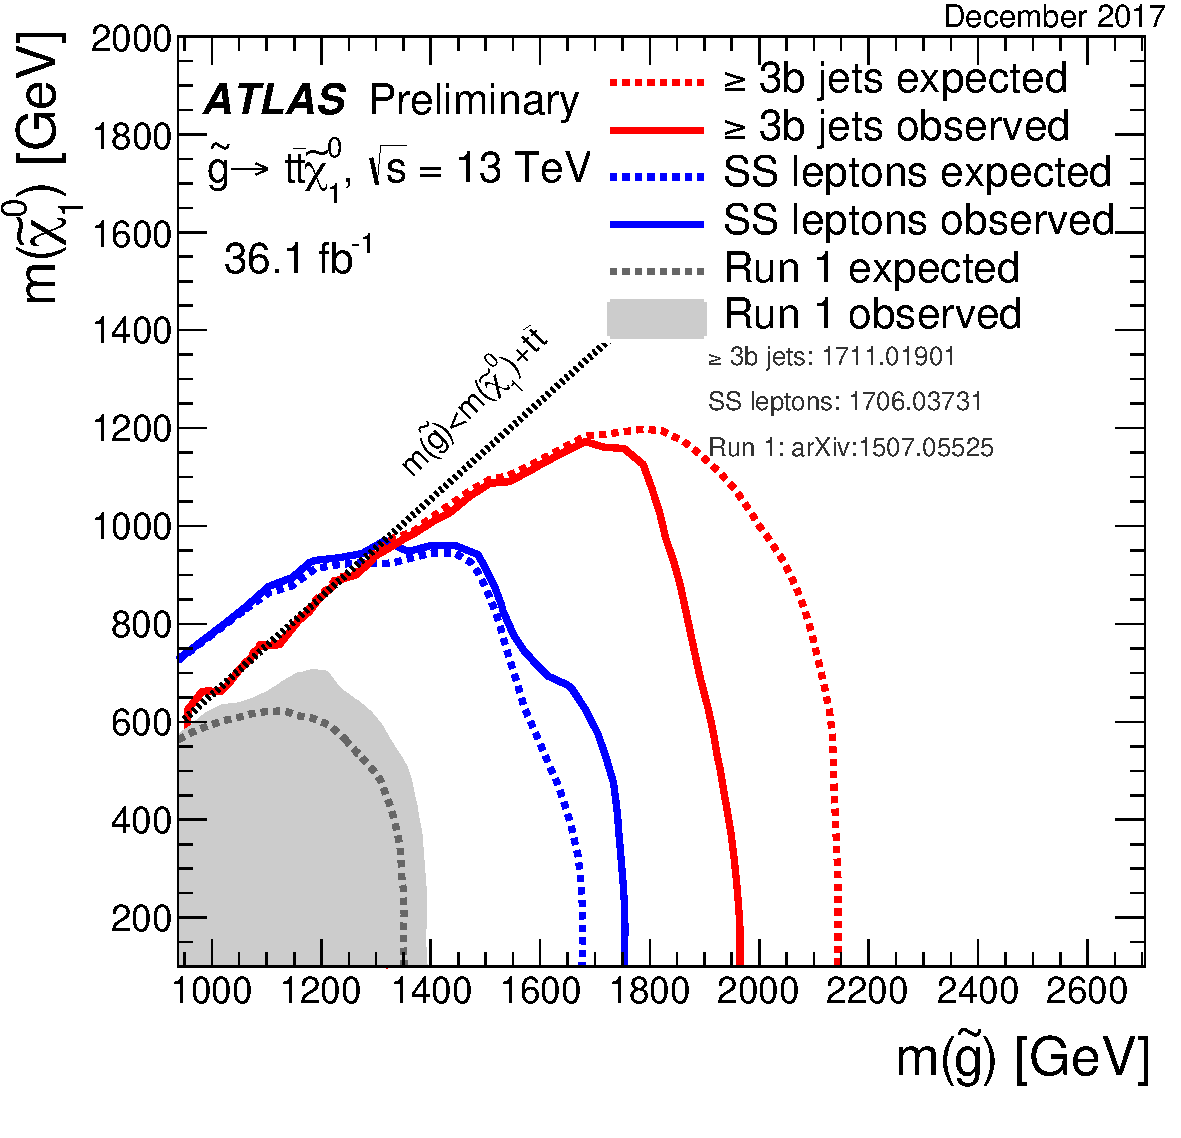
\includegraphics[width=0.65\textwidth]{./fig/limits/ATLAS_SUSY_Gtt.pdf}
\end{center}
\caption[ATLAS Gluino-mediated stop production limits]{ATLAS Gluino-mediated stop production limits in the $(m_{\tilde{g}}, m_{\tilde{chi}_1^0})$ plane.}
\label{fig:ATLASgluinolimits}
\end{figure}

\subsubsection{Direct stop pair production}

Figure \ref{fig:ATLASstoplimits} shows a summary of the dedicated ATLAS searches for top squark (stop) pair production based on 20 \ifb of p-p collision data taken at \cmotto TeV, and 4.7 \ifb of p-p collision data taken at \cmotto TeV \cite{atlas:stop0lep} \cite{atlas:stop2lep}. Exclusion limits at 95\% CL are shown in the $\left( m_{\tilde{t}_1}, m_{\tilde{\chi}^+_1} \right)$ plane. The dashed and solid lines show the expected and observed limits, respectively, including all uncertainties except the theoretical signal cross-section uncertainty. Three decay modes are considered separately with 100\% BR: 

\begin{itemize}
\item $\tilde{t} \rightarrow t \tilde{\chi}^0_1$ (7 TeV: \cite{atlas:stoplim_1} \cite{atlas:stoplim_2} \cite{atlas:stoplim_3}, 8 TeV \cite{atlas:stoplim_4} \cite{atlas:stoplim_5} \cite{atlas:stoplim_6}, where the $\tilde{t}_1$ is mostly right-handed)


\item $\tilde{t} \rightarrow W b  \tilde{\chi}^0_1$ (3-body decay for $m_{\tilde{t}} < m_t + m_{\tilde{\chi}^0_1} $, 8 TeV \cite{atlas:stoplim_4}\cite{atlas:stoplim_6}) 

\item  $\tilde{t} \rightarrow f f' b  \tilde{\chi}^0_1$ (4-body decay, 8 TeV \cite{atlas:stoplim_4}\cite{atlas:stoplim_7}). The region stop1 mass below 100 GeV has not been considered in \cite{atlas:stoplim_4} for the 4-body decay. 

\end{itemize}

\begin{figure}[htbp]
\begin{center}
%\includegraphics[width=0.65\textwidth]{./fig/limits/ATLAS_SUSY_Stop_tLSP.pdf}
\end{center}
\caption[ATLAS limits on direct stop production]{ATLAS limits on direct stop production in the $\left( m_{\tilde{t}_1}, m_{\tilde{\chi}^+_1} \right)$ plane.}
\label{fig:ATLASstoplimits}
\end{figure}



\subsubsection{Electroweak chargino-neutralino production}

Figure \ref{fig:ATLASewlimits} shows the summary of ATLAS searches for electroweak production of charginos and neutralinos based on 20 \ifb of p-p collision data at \cmotto TeV. Exclusion limits at 95\% confidence level are shown in the $\left( m_{\tilde{\chi}^+_1}, m_{\tilde{\chi}^0_1}  \right)$ plane. The dashed and solid lines show the expected and observed limits, respectively, including all uncertainties except the theoretical signal cross-section uncertainties. Four decay modes of the charginos and neutralinos are considered separately with 100\% branching fraction: 

\begin{itemize}

\item $\tilde{\chi}^+_1 \rightarrow \tilde{l} \nu (\tilde{\nu} l ) \rightarrow l \nu \tilde{\chi}^0_1 $, $\tilde{\chi}^0_2  \rightarrow \tilde{l} l (\tilde{\nu} \nu ) \rightarrow l l \tilde{\chi}^0_1 ( \nu \nu \tilde{\chi}^0_1  )$, resulting in BR(3 leptons)=50\% and BR(2 leptons)=100\% for $\tilde{\chi}^+_1 + \tilde{\chi}^0_2$ and $\tilde{\chi}^+_1 + \tilde{\chi}^+_1$ productions, respectively. The decays via sleptons and sneutrinos occur with 50\% probability each. 

\item $\tilde{\chi}^+_1 \rightarrow \tilde{\tau} \nu_{\tau} \tilde{\nu} \rightarrow \tau \nu \tilde{\chi}^0_1$,  $\tilde{\chi}^0_2  \rightarrow \tilde{\tau} \tau ( \tilde{\nu} \nu ) \rightarrow \tau \tau \tilde{\chi}^0_1 ( \nu \nu \tilde{\chi}^0_1   ) $, resulting in BR(3 taus)=50\% and BR(2 taus)=100\% for $\tilde{\chi}^+_1 + \tilde{\chi}^0_2$ and $\tilde{\chi}^+_1 + \tilde{\chi}^+_1$ productions respectively. The decays via staus and tau sneutrinos occur with 50\% probability each. 

\item $\tilde{\chi}^+_1 \rightarrow W  \tilde{\chi}^0_1$, $\tilde{\chi}^0_2  \rightarrow Z \tilde{\chi}^0_1$.

\item $\tilde{\chi}^+_1 \rightarrow W  \tilde{\chi}^0_1$, $\tilde{\chi}^0_2  \rightarrow H \tilde{\chi}^0_1$, where H is the Higgs boson and decays with the SM branching ratios.

\end{itemize}

\begin{figure}[htbp]
\begin{center}
%\includegraphics[width=0.65\textwidth]{./fig/limits/ATLAS_SUSY_EWSummary.pdf}
\end{center}
\caption[ATLAS Electroweak chargino-neutralino production limits]{ATLAS limits for Electroweak chargino-neutralino production in the $\left( m_{\tilde{\chi}^+_1}, m_{\tilde{\chi}^0_1}  \right)$ plane.}
\label{fig:ATLASewlimits}
\end{figure}

\begin{figure}[p]
\begin{center}
%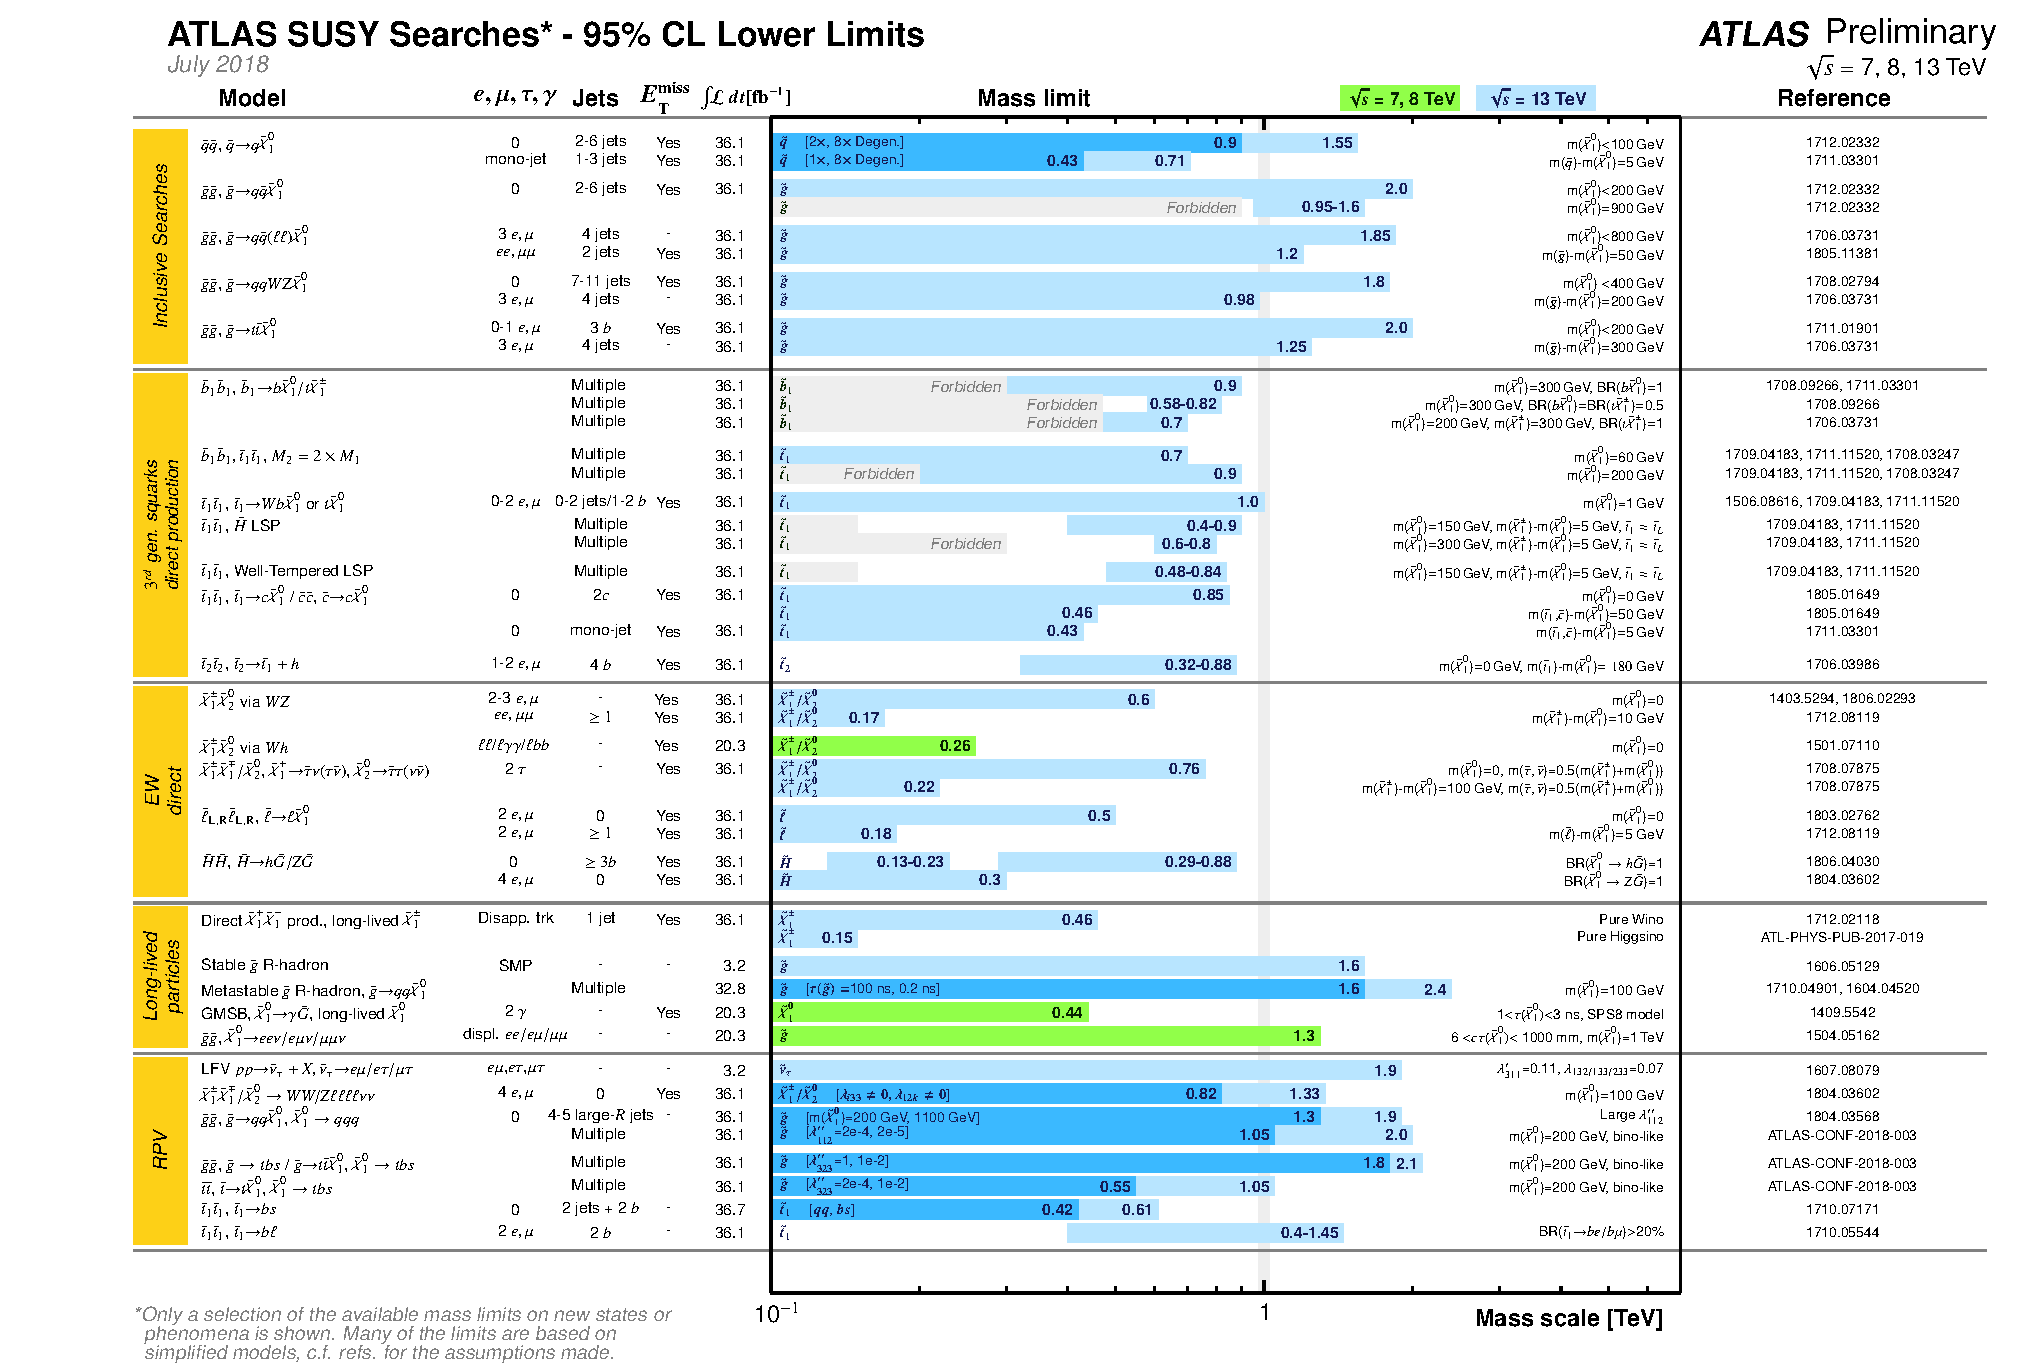
\includegraphics[width=\textwidth]{./fig/limits/ATLAS_SUSY_Summary.pdf}
\end{center}
\caption[Mass reach of ATLAS searches for Supersymmetry]{Mass reach of ATLAS searches for Supersymmetry.}
\label{fig:SUSYlimits}
\end{figure}


%%%%%%%%%%%%%%%%%%%%%%%%%%%%%%%%%%%%%%%%%%
%%%%%%%%%%%%%%%%%%%%%%%%%%%%%%%%%%%%%%%%%%







\chapter{Standard Model and Supersymmetry}
\label{chap:SMSUSY}

This chapter presents an introduction to the \gls{sm} of particle physics, the theory that nowadays best describes the subatomic world. In Section \ref{sec:smsusy:sm} a general overview of the \gls{sm} is given. Section \ref{sec:smsusy:bsm} discusses the limitations of the SM, and some of the theoretical extensions proposed to overcome them. Finally Section \ref{sec:smsusy:susy} focuses on Supersymmetry, arguably one of the most promising of these extensions. Throughout this chapter (as well as in the rest of this thesis) we will use natural units; we will thus use energy units to describe masses, as the speed of light ($c$) and the Planck constant ($\hslash$) are set to unity.


\section{The Standard Model of Particle Physics}
\label{sec:smsusy:sm}

The \gls{sm} is a renormalizable gauge quantum field theory based on the group $SU(3) \times SU(2) \times U(1)$. It was developed in the second half of the 20th century \cite{Glashow:1961tr, Weinberg:1967tq, Salam:1980jd}, and since then the description that it gives of the elementary particles and of their interactions has been accurately tested by several experiments. Many experimental discoveries have been guided by the \gls{sm} predictions, including the discovery of the top quark \cite{Abachi:1994td, PhysRevLett.74.2626} and up to the latest one, the observation of the Higgs boson at the \gls{lhc} in July 2012 \cite{Aad:2012tfa, Chatrchyan:2012xdj}. 

\subsection{Particle content of the Standard Model}

In the \gls{sm}, particles are described as excitations of quantum fields. In the following paragraphs, we introduce the quantum field theory description of fermions and bosons.

\subsubsection*{Fermions}

Matter constituents are half-integer spin fields (fermions). Fermions are further divided into two categories based on the type of interaction they experience:
\begin{description}
\item[Leptons] which experience only the electroweak interaction.
\item[Quarks] which experience both the electroweak and the strong interaction.
\end{description}

Both leptons and quarks come in three generations, and conventionally the numbering of these generations follows an order of increasing mass. A summary of the \gls{sm} fermions is presented in Table \ref{tab:sm_fermions}. While it is possible to observe free leptons, quarks exist only in bound states (hadrons); this is because of the confinement property of the strong interaction, discussed in Section \ref{sec:strong}. Hadrons built of three quarks have spin $\frac{1}{2}$ and are named barions, while mesons are formed by two quarks and have integer spin.


The free Lagrangian of a fermion is given by:

\begin{equation}
 \mathcal{L}_{free} = \bar{\psi} \left( i \gamma^{\mu} \partial_{\mu} - m \right) \psi \, , \
 \label{eq:sm:dirac}
\end{equation}

\noindent where $\psi$ is the fermion field, $m$ its mass, $\gamma$ are the Dirac matrices and $\partial_{\mu}$ is the four-momentum derivative. 

\begin{table}[h]
\centering
\begin{tabular}{c|ccc|ccc}
\hline
 & \multicolumn{3}{c|}{Leptons} & \multicolumn{3}{c}{Quarks} \\
\hline
\hline
Generation & Flavour & Charge & Mass [GeV] & Flavour & Charge & Mass [GeV]\\
\hline
\hline
\multirow{2}*{$1^{st}$} & $\nu_e$ & 0   & $< 2 \times 10^{-9}$  & $u$ & +2/3 & $2.2 \times 10^{-3}$ \\
                        & $e$     & -1  & $5.1 \times 10^{-4}$ & $d$ & -1/3 & $4.8 \times 10^{-3}$ \\
\hline  
\multirow{2}*{$2^{nd}$} & $\nu_\mu$ & 0   & $< 2 \times 10^{-9}$  & $c$ & +2/3 & $ 1.27 $ \\
                        & $\mu$     & -1  & $ 0.10566  $ & $s$ & -1/3 & $ 0.096 $ \\
\hline                 
\multirow{2}*{$3^{rd}$} & $\nu_\tau$ & 0   & $< 2 \times 10^{-9}$  & $t$ & +2/3 & $ 173.2 $ \\
                        & $\tau$     & -1  & $ 1.77 $ & $b$ & -1/3 & $ 4.66 $ \\
\hline  
                 
%\multirow{2}*{Weak} & $W^{+}$, $W^{-}$    &  +1, -1 &  	$80.385$ $\pm0.015$ \\%  & $10^{-6}$\\
 
\end{tabular}
\caption[Standard Model Ferimons]{Fermion content of the Standard Model. Each particle is listed with its electric charge and mass \cite{Patrignani:2016xqp}.} 
\label{tab:sm_fermions}
\end{table}


\subsubsection*{Bosons}

Particles with integer spin are referred to as bosons. In the \gls{sm}, force carriers are described through spin-1 fields. 
The \gls{sm} includes also a spin-0 particle, the Higgs boson. Is the interaction with the Higgs boson field that allows all the other elementary particles to acquire mass, as described in Section \ref{sec:smsusy:ew}.

The Klein-Gordon Lagrangian governs the kinematics of spin-0 neutral particles:

\begin{equation}
\mathcal{L}_{\rm{free}} = \frac{1}{2} \partial^\mu \phi \partial_\mu \phi - \frac{1}{2} m^2 \phi ^2 ,
\end{equation}

 
\noindent while in the case of charged particles (described through a complex field) the Lagrangian becomes:

\begin{equation}
\mathcal{L}_{\rm{free}} =  \partial^\mu \phi \partial_\mu \phi^* -  m^2 \phi \phi^* .
\end{equation}


\noindent The two equations above describe scalar particles. In the case of a vector field $A^\mu$, the expression of the Lagrangian is the following: 

\begin{equation}
\mathcal{L}_{\rm{free}} =  - \frac{1}{4} F^{\mu \nu}F_{\mu \nu} +  \frac{1}{2} m^2 A^\mu A_\mu \, .
\label{eq:lproca}
\end{equation}

\noindent This is the Proca Lagrangian. In the case of a particle with zero mass, this reduces to the Maxwell Lagrangian:

\begin{equation}
\mathcal{L}_{free} =  - \frac{1}{4} F^{\mu \nu}F_{\mu \nu} ,
\label{eq:lmax}
\end{equation}


\noindent where $F^{\mu \nu} = \partial^\mu A_\nu - \partial^\nu A_\mu$.

\subsection{Interactions and gauge invariance}

The \gls{sm} describes all the interactions among elementary particles, except for gravity, for which nowadays no renormalizable quantum field theory is formulated. Table \ref{tab:sm_interazioni} presents a summary of the \gls{sm} interactions and the properties of the corresponding force carriers. More details about the strong and electroweak interactions are given in the following sections.

\begin{table}[h]
\centering
\begin{tabular}{llcc}
\hline
Interaction & Carrier & Electric Charge & Mass [GeV] \\% & $\alpha$ \\
\hline
\hline
Strong & Gluons (g)  & 0 & 0 \\ % & 10 \\
\hline
Electromagnetic & Photon ($\gamma$) & $< 10^{-27}$ & 0 \\%& $10^{-2}$ \\
\hline
\multirow{2}*{Weak} & $W^{+}$, $W^{-}$    &  +1, -1 &  	$80.385$  \\% $\pm0.015$  & $10^{-6}$\\
 & $Z$  & 0 &  	$91.1876$  \\% & $\pm0.0021$ \\
\hline
\end{tabular}
\caption[Interaction in the Standard Model]{Interaction in the Standard Model. Here the different force carriers are listed, with their electric charges and masses \cite{Patrignani:2016xqp}.} %; $\alpha$ is the coupling constant of the different interactions.}
\label{tab:sm_interazioni}
\end{table}


The interaction terms in the \gls{sm} Lagrangian are introduced by promoting an already existing global symmetry of the Lagrangian ($\theta$) to a local one ($\theta(x)$) function of the space-time coordinates. 
In general, given a Lagrangian globally invariant under a symmetry group, the fields transform as:
\begin{equation}
\psi \rightarrow e^{ig\theta_k \tau_k} \psi  \; ,
\end{equation}

\noindent where $g$ is the coupling constant of the filed $\psi$ under the interaction and $\tau_k$ are the generators of the group and obey commutation relations: 
\begin{equation}
\left[ \tau_i, \tau_j \right] = i f_{ijk} \tau^k \; . 
\end{equation}

\noindent $f_{ijk}$ is the structure constant of the group and is always zero for Abelian groups. Promoting this gauge invariance to a global one ($\theta_k \rightarrow \theta_k(x)$) implies adding to the theory:
\begin{itemize}
\item A number of massless gauge fields $W^\mu_k$ equal to the number of generators of the symmetry group, that transform as 
\begin{equation}
W^\mu_k \rightarrow W^\mu_k - \partial^\mu \theta_k - g \epsilon_{klm} \theta^m W^\mu_m \; .
\end{equation}
\item A covariant derivative: 
\begin{equation}
D^\mu = \partial^\mu + ig\tau^kW^\mu_k \; ,
\end{equation}

\noindent that substitutes the standard derivative in the Lagrangian.
\item A free Lagrangian for the vector fields as in Equation \ref{eq:lproca}, with:
\begin{equation}
F^{\mu \nu}_k = \partial_\mu W_k^\nu - \partial_\nu W_k^\mu - g f_k^{lm} W^\mu_l W^\nu_m \; .
\end{equation}
\noindent Note that the last term, of second order in the field, is present only for non-Abelian symmetry groups, since it is proportional to the structure constant. This has non-trivial consequences as the second-order term leads to self-interaction among the gauge fields.
\end{itemize}


The \gls{sm} is a theory invariant under $SU(3)_{C} \times SU(2)_{L} \times U(1)_{Y}$. Imposing local invariance under $SU(3)_{C}$ leads to the theory of strong interactions, while $SU(2)_{L} \times U(1)_{Y}$ is the symmetry whose breaking gives origin to the electroweak interactions. 

\subsection{Strong interaction}
\label{sec:strong}

\gls{qcd} is the theory that describes strong interactions, based on the symmetry group $SU(3)_\mathrm{C}$, where the subscript C refers to the color, the quantum number associated with these interactions; this can assume three possible values denoted with red, blue and green. The observable states, hadrons, are color singlets, while quarks (anti-quarks) carry only one color (anti-color) charge. Since the symmetry group is non-Abelian, also the corresponding eight gauge bosons (gluons) carry a color charge (bi-color, with one color and one different anti-color) and therefore interact not only with quarks but also among themselves. Since $SU(3)_\mathrm{C}$ is believed to be an exact symmetry,  gluons are massless. 

The renormalization of a gauge theory leads to the definition of running coupling constants, whose value depend on the energy scale at which they are evaluated. In \gls{qcd}, at leading order the dependence of the coupling constant on the energy scale $Q$ is given by:

\begin{equation}
\alpha_\mathrm{s}(Q^2)=\frac{12\pi}{\left(11N_\mathrm{C}-2n_\mathrm{f}\right)\log{\frac{Q^2}{\Lambda_\mathrm{QCD}^2}}} \; , 
\label{eq:alfaQCD}
\end{equation}

\noindent where $N_\mathrm{C}$ is the number of colors, $n_\mathrm{f}$ is the number of quark flavors that are active (i.e. whose mass is lower than the energy scale) and $\Lambda_\mathrm{QCD}$ is the infrared cutoff scale that sets the limit of validity of the perturbative approximation. In \gls{qcd} $N_\mathrm{C} = 3$, so for $n_\mathrm{f}<16$ the coupling constant decreases with the increase of the energy scale of the process considered. This behavior has important consequences on the properties of the strong interaction:

\begin{itemize}
\item At high $Q^2$ (i.e. at small distances), $\alpha_\mathrm{s}$ becomes small enough for the perturbative approximation to be correct. In this case quarks and gluons behave as free particles (asymptotic freedom) \cite{PhysRevLett.30.1343, PhysRevLett.30.1346}.
\item When the momentum transfer is small (i.e. at large distances) $\alpha_\mathrm{s}$ is large; this gives rise to confinement: quarks can not be observed as isolated particles, as it is not possible to extract individual quarks from hadrons. When the distance between two quarks is increased, the potential energy increases as well, up to the point when it is energetically more favorable to create from the vacuum a quark-antiquark pair and thus a new hadron is formed.
\item In a collider experiment, quarks and gluons will create a collimated spray of hadrons (jets).
\end{itemize}

The evolution of the \gls{qcd} coupling constant with the energy scale has been verified experimentally, as shown in Figure \ref{fig:sm:alphas} \cite{Bethke:2012jm}.

\begin{figure}[ht]
\centering
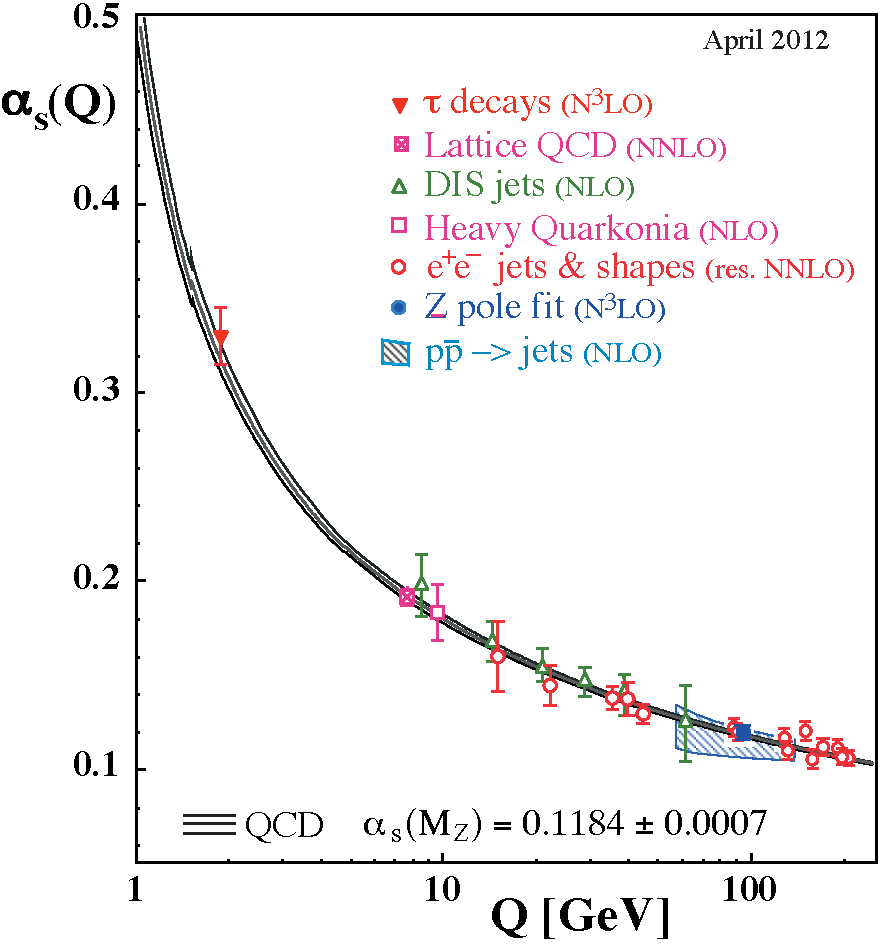
\includegraphics[width=0.5\textwidth]{figures/theory/asq-2011}
\caption{Evolution of the \gls{qcd} coupling constant $\alpha_\mathrm{s}$ with the energy scale. Figure from Ref \cite{Bethke:2012jm}.}
\label{fig:sm:alphas}
\end{figure}

\subsection{Electroweak interaction and Higgs-Englert-Brout mechanism}
\label{sec:smsusy:ew}

The theory of electroweak interactions is based on the symmetry group $SU(2)_\mathrm{L} \times U(1)_\mathrm{Y}$. This symmetry breaks at a scale around 100 GeV giving rise to the electromagnetic interaction, mediated by the photon, and to the weak interaction, mediated by the $Z$ and $W^{\pm}$ bosons  for neutral currents and charged currents respectively. The number of mediators, four, is the same as the number of generators of the symmetry group. 

The $SU(2)_\mathrm{L}$ part of the symmetry group governs the weak interactions, and the subscript L indicates that only left-handed particles participate to them. Left-handed and right-handed fields ($\psi_L$ and $\psi_R$ respectively) are defined through the chirality projectors $P_L$ and $P_R$:

\begin{equation}
\begin{aligned}
\psi_L = P_L \psi = \frac{(1 - \gamma_5)}{2} \psi, \\
\psi_R = P_R \psi = \frac{(1 + \gamma_5)}{2} \psi,
\end{aligned}
\label{eq:sm:LR}
\end{equation}

\noindent where $\gamma_5$ is defined as $\gamma_5 = i \gamma^0 \gamma^1 \gamma^2 \gamma^3 $. Looking back at Equation \ref{eq:sm:dirac}, it can be noted that, if we decompose the fermion field into its left-handed and right-handed components, the derivative term keeps $\psi_L$ and $\psi_R$ separated, while the mass term mixes them:
\begin{equation}
-m \bar \psi \psi = -m \bar \psi P_L^2 \psi - m \bar \psi P_R^2 \psi
	= -m \bar \psi_R \psi_L - m \bar \psi_L \psi_R \; .
\end{equation}


\noindent The covariant derivative for the  $SU(2)_\mathrm{L} \times U(1)_\mathrm{Y}$ group is:
\begin{equation}
\mathcal{D}^{\mu} = \partial^{\mu} + i \frac{g'}{2} B^\mu Y + ig W^\mu_k T^k \; ,
\label{eq:sm:covD}
\end{equation}

\noindent and substituting with this the regular derivative results in the interaction Lagrangian:
\begin{equation}
\mathcal{L}_{int}^{EW} = -\frac{g'}{2} \left( \bar{\psi} \gamma_\mu Y \psi \right) B^\mu - g \sum_k \left( \bar{\psi} \gamma_\mu T^k \psi  \right) W_k^\mu \; ,
\end{equation}

\noindent where we have introduced $T^k$, the weak isospin operator, and $Y$, the hypercharge operator (associated to the $U(1)_\mathrm{Y}$ group), and the respective coupling constants $g$ and $g'$. The quantum numbers of the $T^k$ and $Y$ operators relate to the electric charge $Q$ through the  Gell-Mann Nishijima relation:

\begin{equation}
Q = \frac{Y}{2} + T_3
\label{eq:sm:Q}
\end{equation}

\noindent where $Y$ is the hypercharge quantum number and $T_3$ is the quantum number of the third component of the isospin. 

In the case of an $SU(2)$ symmetry, it is not possible to add directly to the Lagrangian a mass term for the vector bosons of the form in Equation \ref{eq:lproca}, as it would spoil the $SU(2)$ local invariance. The Higgs-Englert-Brout mechanism \cite{Englert:1964et, Higgs:1964pj, Higgs:1964ia} solves this problem through \gls{ssb} of the $SU(2)_\mathrm{L} \times U(1)_\mathrm{Y}$ invariance. The \gls{ssb} is obtained by adding to the theory one extra isospin doublet of complex scalar components, the Higgs field:

\begin{equation}
	\Phi = \left( \begin{array}{c} \phi^+  \\ \phi^0 \end{array} \right) \; .
\end{equation}
%	= \frac{1}{\sqrt{2}} \left( \begin{array}{c} \phi_1 + i \phi_2 \\ \phi_3 + i \phi_4 \end{array} \right)

\noindent This doublet has hypercharge $Y=1$ and isospin $T=\frac{1}{2}$; the first component has positive electric charge, while the second one is electrically neutral. The Lagrangian for this new field includes a kinetic and a potential term:

\begin{equation}
	\mathcal{L}_{\Phi} = ( \mathcal{D}_{\mu} \Phi)^{\dagger} (\mathcal{D}^{\mu} \Phi) - V(\Phi) \; ,
	\label{eq:LHiggs}
\end{equation}

\noindent where $\mathcal{D}_{\mu}$ is the covariant derivative defined in Equation \ref{eq:sm:covD} and the potential $V(\Phi)$ is given by:

\begin{equation}
 V(\Phi) =  \mu^2 \Phi^{\dagger} \Phi + \lambda (\Phi^{\dagger} \Phi)^2 \, . 
	\label{eq:hpot}
\end{equation}

\noindent The two real parameters $\mu^2$ and $\lambda$ relate respectively to the mass term and the strength of the self-interaction term. The shape of the potential depends on the value of these parameters:
\begin{itemize}
\item If $\lambda < 0$, the potential does not present any stable minima, and this case is therefore unphysical.
\item If $\lambda > 0$ and $\mu^2 > 0$ there is only one solution to the minimization of the potential, $\Phi=0$. This case is shown in Figure  \ref{fig:sm:HiggsV_1}.
\item If $\lambda > 0$ and $\mu^2 < 0$, the field acquires a \gls{vev} as the minima is not at zero; it lies instead on the points of the circumference such that:
\begin{equation}
\Phi^{\dagger} \Phi = \frac{\mu^2}{2 \lambda}  \equiv \frac{v^2}{2} \; .
\end{equation}
\noindent Figure \ref{fig:sm:HiggsV_2} illustrates this case.
\end{itemize}


\begin{figure}[ht]
\centering
\subfigure[]{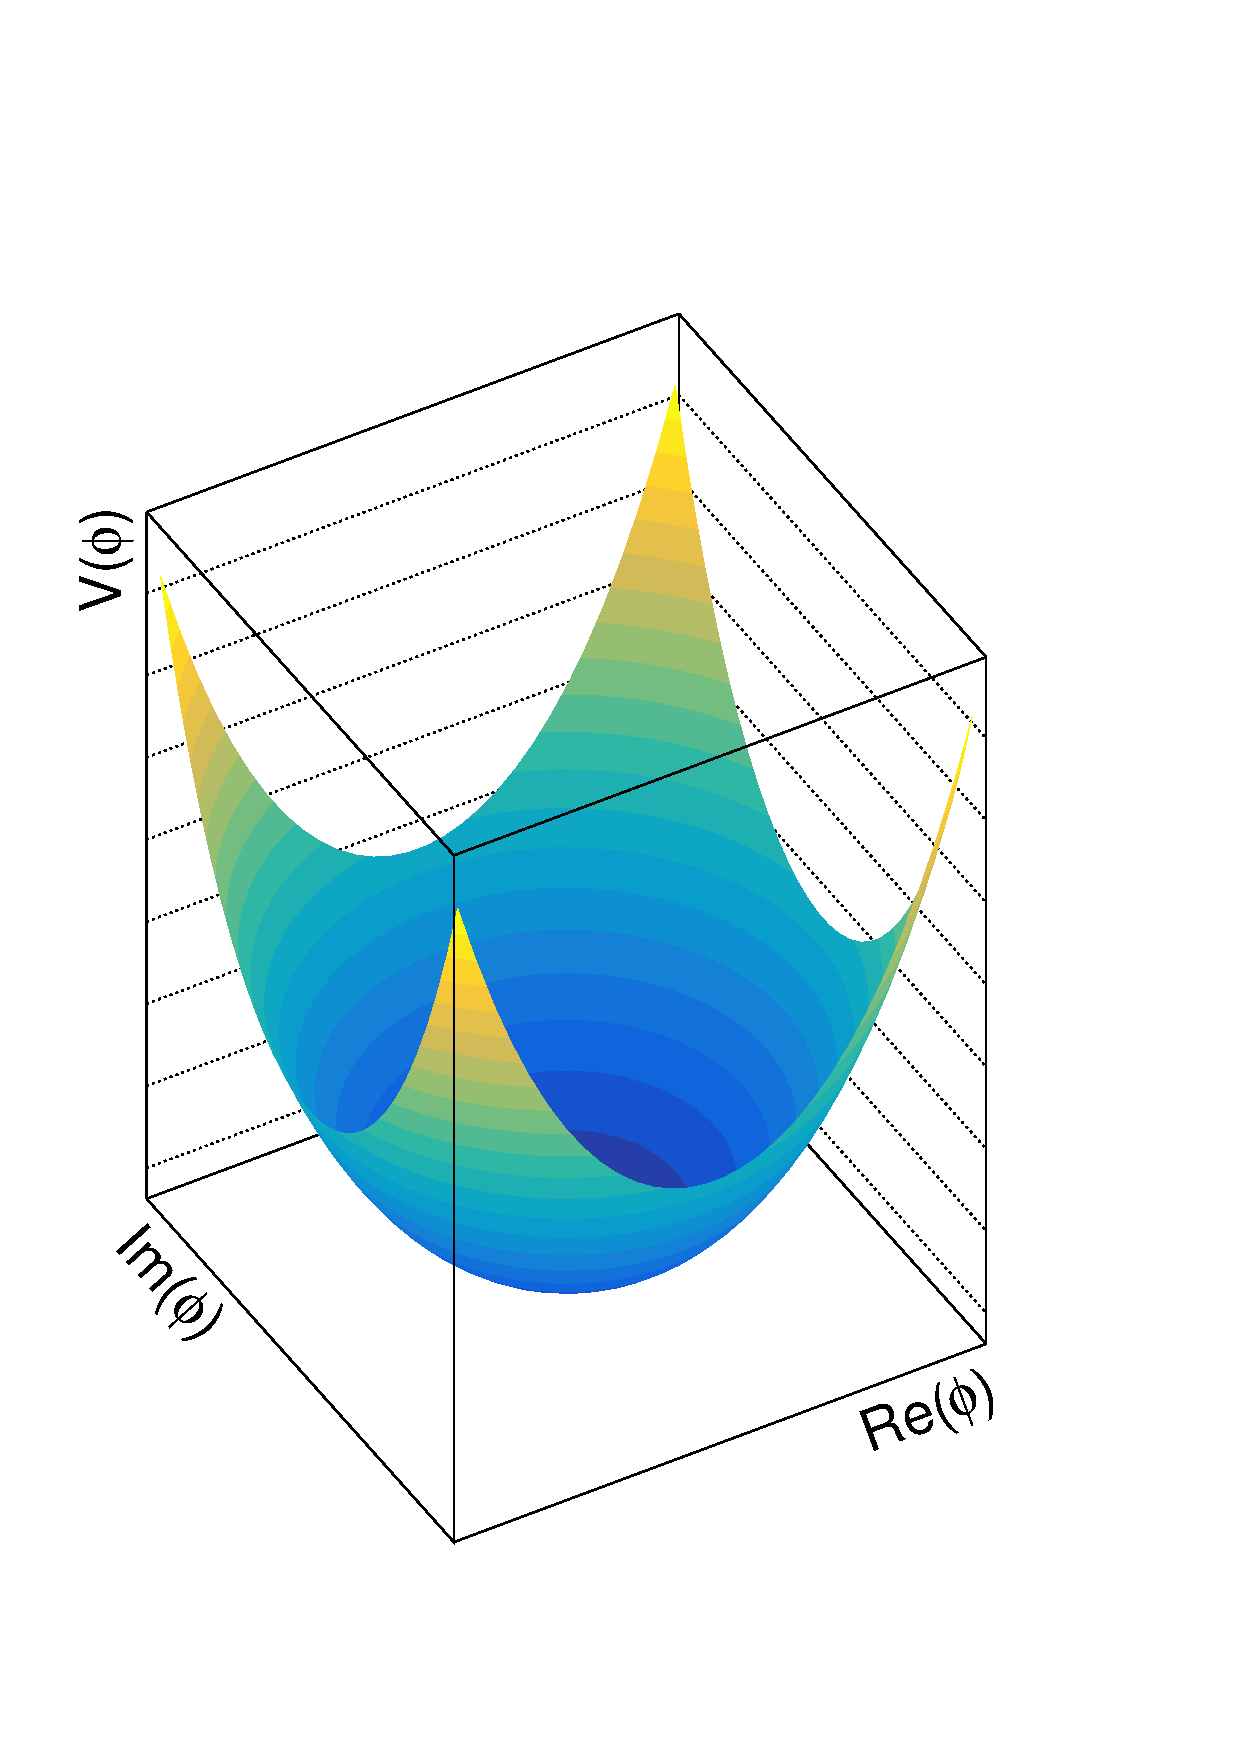
\includegraphics[width=0.49\textwidth]{produce_plots/sm/higgs_posmu2.pdf}\label{fig:sm:HiggsV_1}}
\subfigure[]{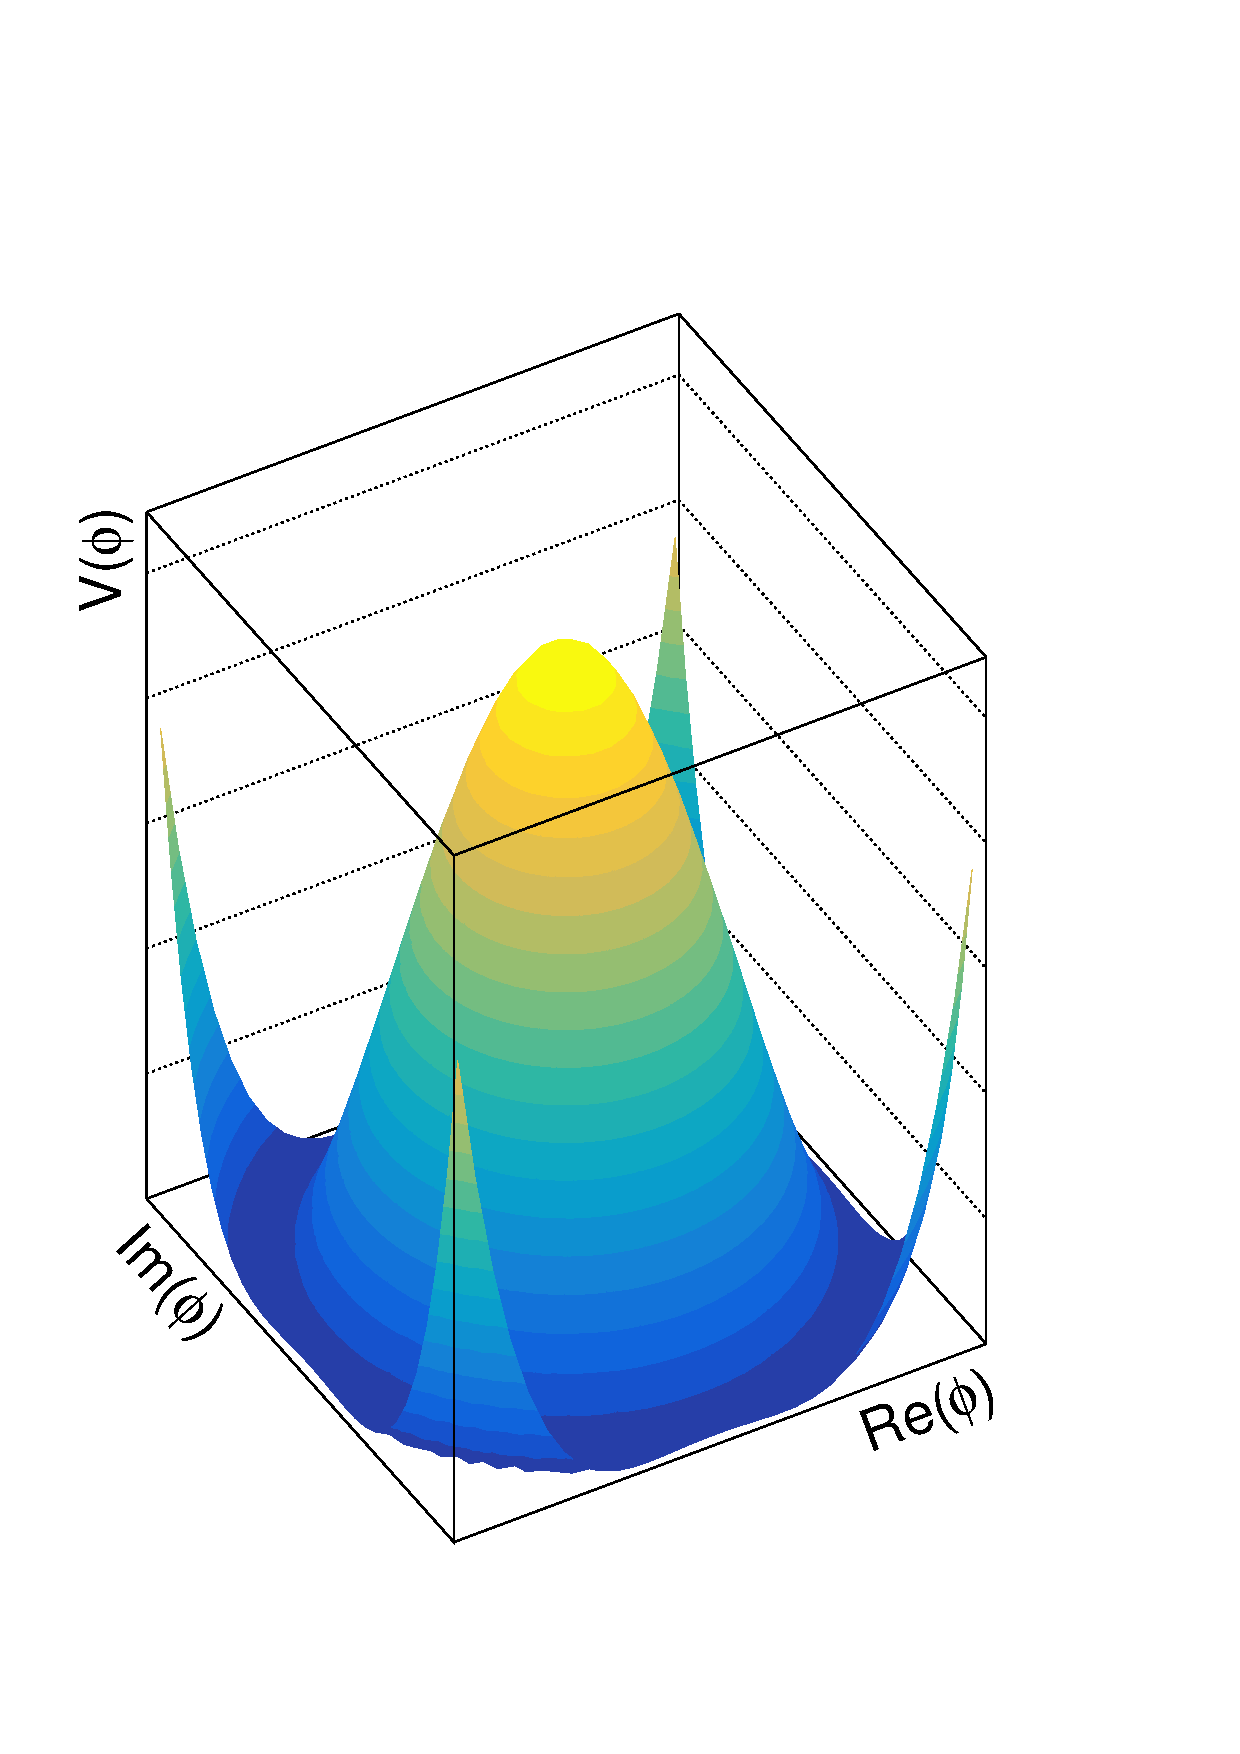
\includegraphics[width=0.49\textwidth]{produce_plots/sm/higgs_negmu2.pdf}\label{fig:sm:HiggsV_2}}
\caption{Higgs potential in the case \subref{fig:sm:HiggsV_1} $\lambda > 0$ and  $\mu^2 > 0$ and \subref{fig:sm:HiggsV_2} $\lambda > 0$ and $\mu^2 < 0$.}
\label{fig:sm:HiggsV}
\end{figure}

Up to this point the $SU(2)_\mathrm{L} \times U(1)_\mathrm{Y}$ symmetry is still intact, but the explicit choice of one of the infinite possible vacuum states for the Higgs field breaks the symmetry. According to the Goldstone theorem \cite{Goldstone:1962es}, the breaking of a continuous symmetry leads to the appearance of new massless scalar particles as field excitations. These new degrees of freedom are absorbed by the existing gauge bosons, thus giving them mass. To meet the experimental requirement of a massless photon, the choice of the Higgs vacuum has not to break the electromagnetic symmetry, $U(1)_{EM}$, so the component of the Higgs doublet that acquires a \gls{vev} is the neutral one:

\begin{equation}
	\Phi_0 = \frac{1}{\sqrt{2}} \left( \begin{array}{c} 0 \\ v  \end{array} \right) \, . \
\label{eq:hvphi}
\end{equation}

We can then expand the field $\Phi$ considering small excitations around the minimum:

\begin{equation}
	\Phi = \frac{e^{i \vec{\sigma} \cdot \vec{\theta}(x)/v }}{\sqrt{2}} \left( \begin{array}{c} 0 \\ v + \phi(x) \end{array} \right) \, ,
\label{eq:hvphi}
\end{equation}

\noindent where $\phi(x)$ is the physical field associated with the Higgs boson, $\vec{\sigma}$ the Pauli matrices and $\vec{\theta}(x)$ the three degrees of freedom absorbed to give masses to the $Z$ and $W^\pm$ bosons. Inserting Equation \ref{eq:hvphi} into Equation \ref{eq:LHiggs} relates the mass of the Higgs boson to the parameters in the potential:
\begin{equation}
m_H = \sqrt{- 2 \mu^2} = \sqrt{2 \lambda} v \; .
\label{eq:sm:Higgsmass}
\end{equation}

Since the numeric value of the $\mu^2$ and $\lambda$ parameters is not set, the theory does not predict a specific value for $m_H$. 
The physical mass eigenstates of the gauge bosons are a rotation of the interaction eigenstates, given by:

\begin{equation}
\begin{aligned}
W_\mu^\pm &= \frac{W_\mu^1 \mp W_\mu^2}{\sqrt{2}} \; , \\
A_\mu &= B_\mu \cos\theta_W + W^3_\mu \sin\theta_W \; ,  \\
Z_\mu &= W^3_\mu \cos\theta_W - B_\mu \sin\theta_W \; ,
\end{aligned}
\label{eq:wein}
\end{equation}

\noindent where we have introduced the Weinberg angle $\theta_W$ such that:
\begin{equation}
\tan\theta_W \equiv \frac{g'}{g} \; .
\end{equation}


The $(\mathcal{D}_{\mu} \Phi)^{\dagger} (\mathcal{D}^{\mu} \Phi)$ term in Equation \ref{eq:LHiggs} gives rise to the physical mass of the gauge bosons: once applied to the Higgs field, the covariant derivative in Equation \ref{eq:sm:covD} produces terms quadratic in the gauge fields, that we interpret as mass terms:

\begin{equation}
\mathcal{L}_{\Phi} = \left(1+\frac{\phi}{v}\right)^2 \,
\left\{ m_W^2\, W_\mu^\dagger W^\mu
+ \frac{1}{2}\, m_Z^2\, Z_\mu Z^\mu \right\}\, +\, \mathcal{L}_H \; , 
\end{equation}

\noindent where $\mathcal{L}_H$ denotes all the terms in $\mathcal{L}_{\Phi}$ that involve only the Higgs field: Higgs boson mass, cubic and quadratic self-interaction. Note that the coupling of the gauge bosons with the Higgs field is proportional to the square of the boson mass.
At tree level the resulting masses of the gauge bosons are:

\begin{equation}
\begin{aligned}
m_\gamma &= 0 \; ,\\
m_Z &= \frac{v \sqrt{g^2 + g'^2}}{2} \; , \\
m_W &= \frac{vg}{2} =  \cos\theta_W m_Z \; .
\end{aligned}
\end{equation}


Therefore, the Higgs-Englert-Brout mechanism generates automatically a mass term for the gauge bosons, that does not break the global underlying $SU(2)_\mathrm{L} \times U(1)_\mathrm{Y}$ symmetry. The Higgs field is used also to make fermion mass terms arise, but in this case it is necessary to postulate a Yukawa interaction between the Higgs and fermion fields. The fermion masses are assumed to be proportional to the strength of the coupling and, unlike the masses of the gauge bosons, they are not related to other parameters of the theory. While the Higgs field itself is enough to give mass to down-type fermions, the mass term for the up-type fermions  requires the introduction of the complex conjugate of the Higgs field ($\Phi_C$):

\begin{equation}
 \Phi_C = i \sigma^2 \Phi^* 
	= i \left( \begin{array}{cc} 0 & -i \\ i & 0 \end{array} \right) 
	\left( \begin{array}{c} \phi^- \\ \phi^{0*} \end{array} \right)
	= \left( \begin{array}{c} \phi^{0*} \\ - \phi^- \end{array} \right) \; ,
\end{equation}

\noindent If we identify as $g_f$ the coupling of the fermion $f$ to the Higgs field (Yukawa coupling), the additional part of the Lagrangian that generates the fermion masses is:

\begin{equation}
\begin{aligned}
\mathcal{L}_{Yukawa} &= - \left[  y_d \left( \bar{u}_L \,\, \bar{d}_L  \right) \Phi d_R +  y_u \left( \bar{u}_L \,\, \bar{d}_L  \right) \Phi_C u_R \right] + h.c. \\
&= - \frac{1}{\sqrt{2}} \left[  y_d \left( v + \phi \right) \bar{d}_L d_R + h.c. + y_u \left( v + \phi \right) \bar{u}_L d_u + h.c. \right]  \; .
\end{aligned}
\end{equation}

\noindent In this equation we can now easily identify the fermion mass terms, of the form:

\begin{equation}
m_f =  \frac{v}{\sqrt{2}} y_f \; .
\end{equation}

\noindent Note that, in the case of fermions, the coupling to the Higgs boson is directly proportional to the fermion mass.The matrices $y_f$ are not necessarily diagonal, but they can be diagonalized through a unitary transformation, which we can interpret as the transformation that relates the mass eigenstates to the weak interaction eigenstates. In the quark sector, this transformation is encoded in the \gls{ckm} matrix \cite{Cabibbo:1963yz, Kobayashi:1973fv}, that describes the mixing of the down-type quarks. In the \gls{sm} with three generations of fermions, the \gls{ckm} matrix is specified by three angles and one complex phase that provides the only source of CP violation.

\subsection{Measured properties of the Higgs boson}

The value of the Higgs boson mass is not predicted by the \gls{sm}, but it can be measured and, once it is know, the Higgs boson production cross-section and decay fractions can be predicted accurately. These predictions can be verified experimentally, providing hints toward believing that the discovered boson is indeed the \gls{sm} Higgs boson. In 2015 the ATLAS and CMS collaborations published a combined measurement of the Higgs boson mass \cite{Aad:2015zhl}:
\begin{equation}
m_H = 125.09 \pm 0.21 (\mathrm{stat.}) \pm 0.11 (\mathrm{syst.}) \;\; \mathrm{GeV}.
\end{equation}

\noindent This result uses the full Run 1 ATLAS and CMS data, analyzed in the $h \rightarrow \gamma \gamma$ and $h \rightarrow ZZ \rightarrow 4 \; \mathrm{leptons}$ channels.


The discussion of the Higgs mechanism in Section \ref{sec:smsusy:ew} highlights interesting properties of the interactions involving the Higgs boson. In particular, the strength of its coupling with fermions and bosons is proportional respectively to the mass and the square of the mass of the particle involved. 
This is reflected on the \glspl{br}: they are high for the decay to particles with the highest mass that are kinematically allowed.
While the top quark mass is too large to have the decay $h \to t\bar{t}$, the large top Yukawa coupling leads to loop-induced couplings of the Higgs boson to massless particles (gluons and photons); these are of phenomenological interest as they lead to the main production mode (gluon-gluon fusion) and to the $h \to \gamma \gamma$ decay mode, which has a low \gls{br} but leads to a very clean signature and was one of the key channels for the Higgs boson discovery. 
%The theoretical \glspl{br} for a Higgs boson mass of 125.09 GeV are reported in Table \ref{tab:SMBranchingFractions}. 

%\begin{table}[htbp]
%\begin{center}
%\begin{tabular}{clcr@{\hskip 0.4ex}l} \\ 
%\hline
% &    Decay mode &\multicolumn{3}{c}{Branching fraction [\%]}  \\  \hline
% \hline
% &     $H \rightarrow b\bar{b}$       & &   $57.5$&${}\pm 1.9$    \\
% &     $H \rightarrow WW$       & &   $21.6$&${}\pm 0.9$   \\
% &     $H \rightarrow gg$       & &   $8.56$&${}\pm 0.86$  \\
% &     $H \rightarrow \tau \bar{\tau}$       & &   $6.30$&${}\pm 0.36$  \\
% &     $H \rightarrow c\bar{c}$       & &   $2.90$&${}\pm 0.35$  \\
% &     $H \rightarrow ZZ$       & &   $2.67$&${}\pm 0.11$  \\
% &     $H \rightarrow \gamma \gamma$       & &   $0.228$&${}\pm 0.011$  \\
% &     $H \rightarrow Zg$       & &   $0.155$&${}\pm 0.014$  \\
% &     $H \rightarrow \mu \bar{\mu}$       & &   ~~$0.022$&${}\pm 0.001$  \\ 
%\hline
%\end{tabular} 
%\end{center}
%\caption{Standard Model predictions for the decay \glspl{br} of a Higgs boson with a mass of 125.09~GeV, together with their uncertainties~\cite{Heinemeyer:2013tqa}. Table follows Ref. \cite{Khachatryan:2016vau}.}
%\label{tab:SMBranchingFractions}
%\end{table} 
The theoretical production cross-section and \glspl{br} for a Higgs boson with mass between 120 and 130 GeV are reported in Figure \ref{fig:sm:h_xsec_br}.

\begin{figure}[ht]
\centering
\subfigure[]{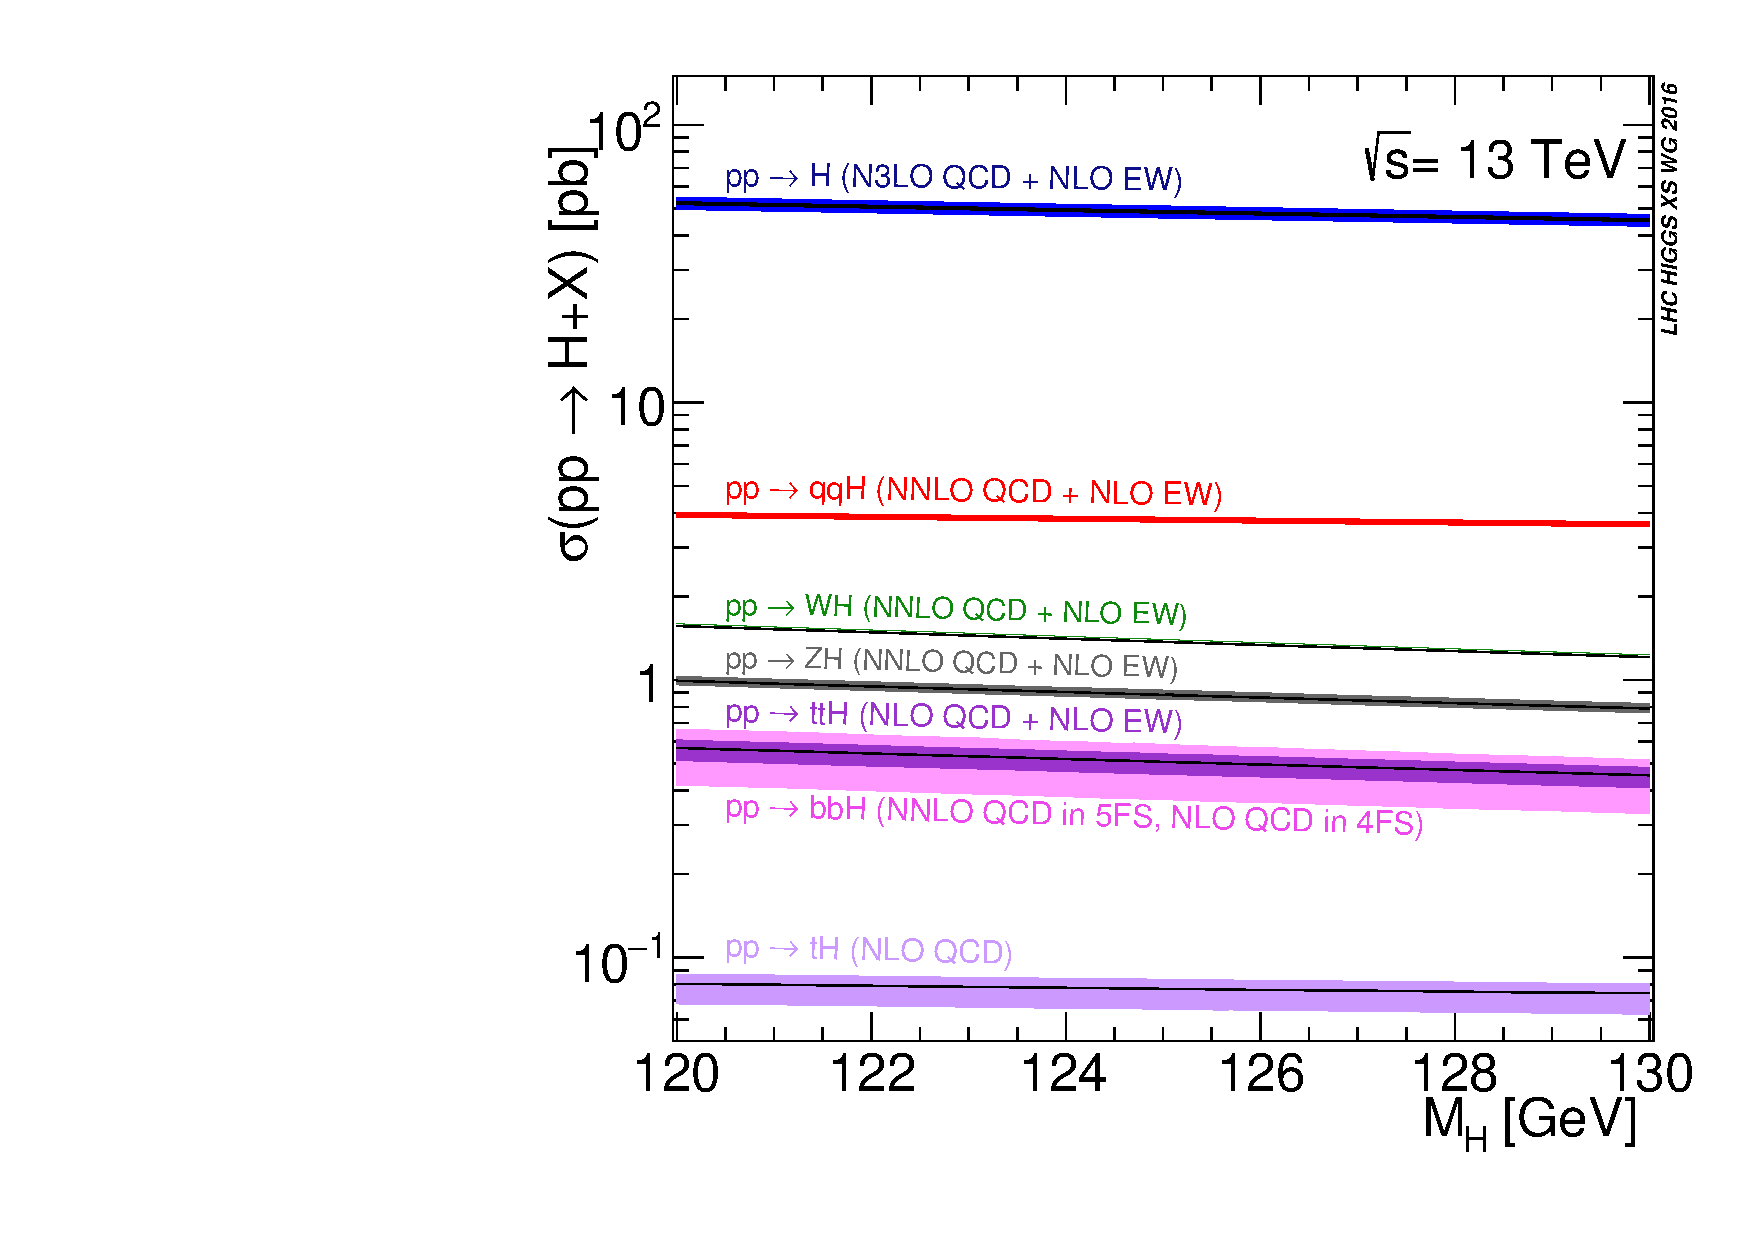
\includegraphics[width=0.49\textwidth]{figures/theory/plot_13tev_H_sqrt}\label{fig:sm:h_xsec_theo}}
\subfigure[]{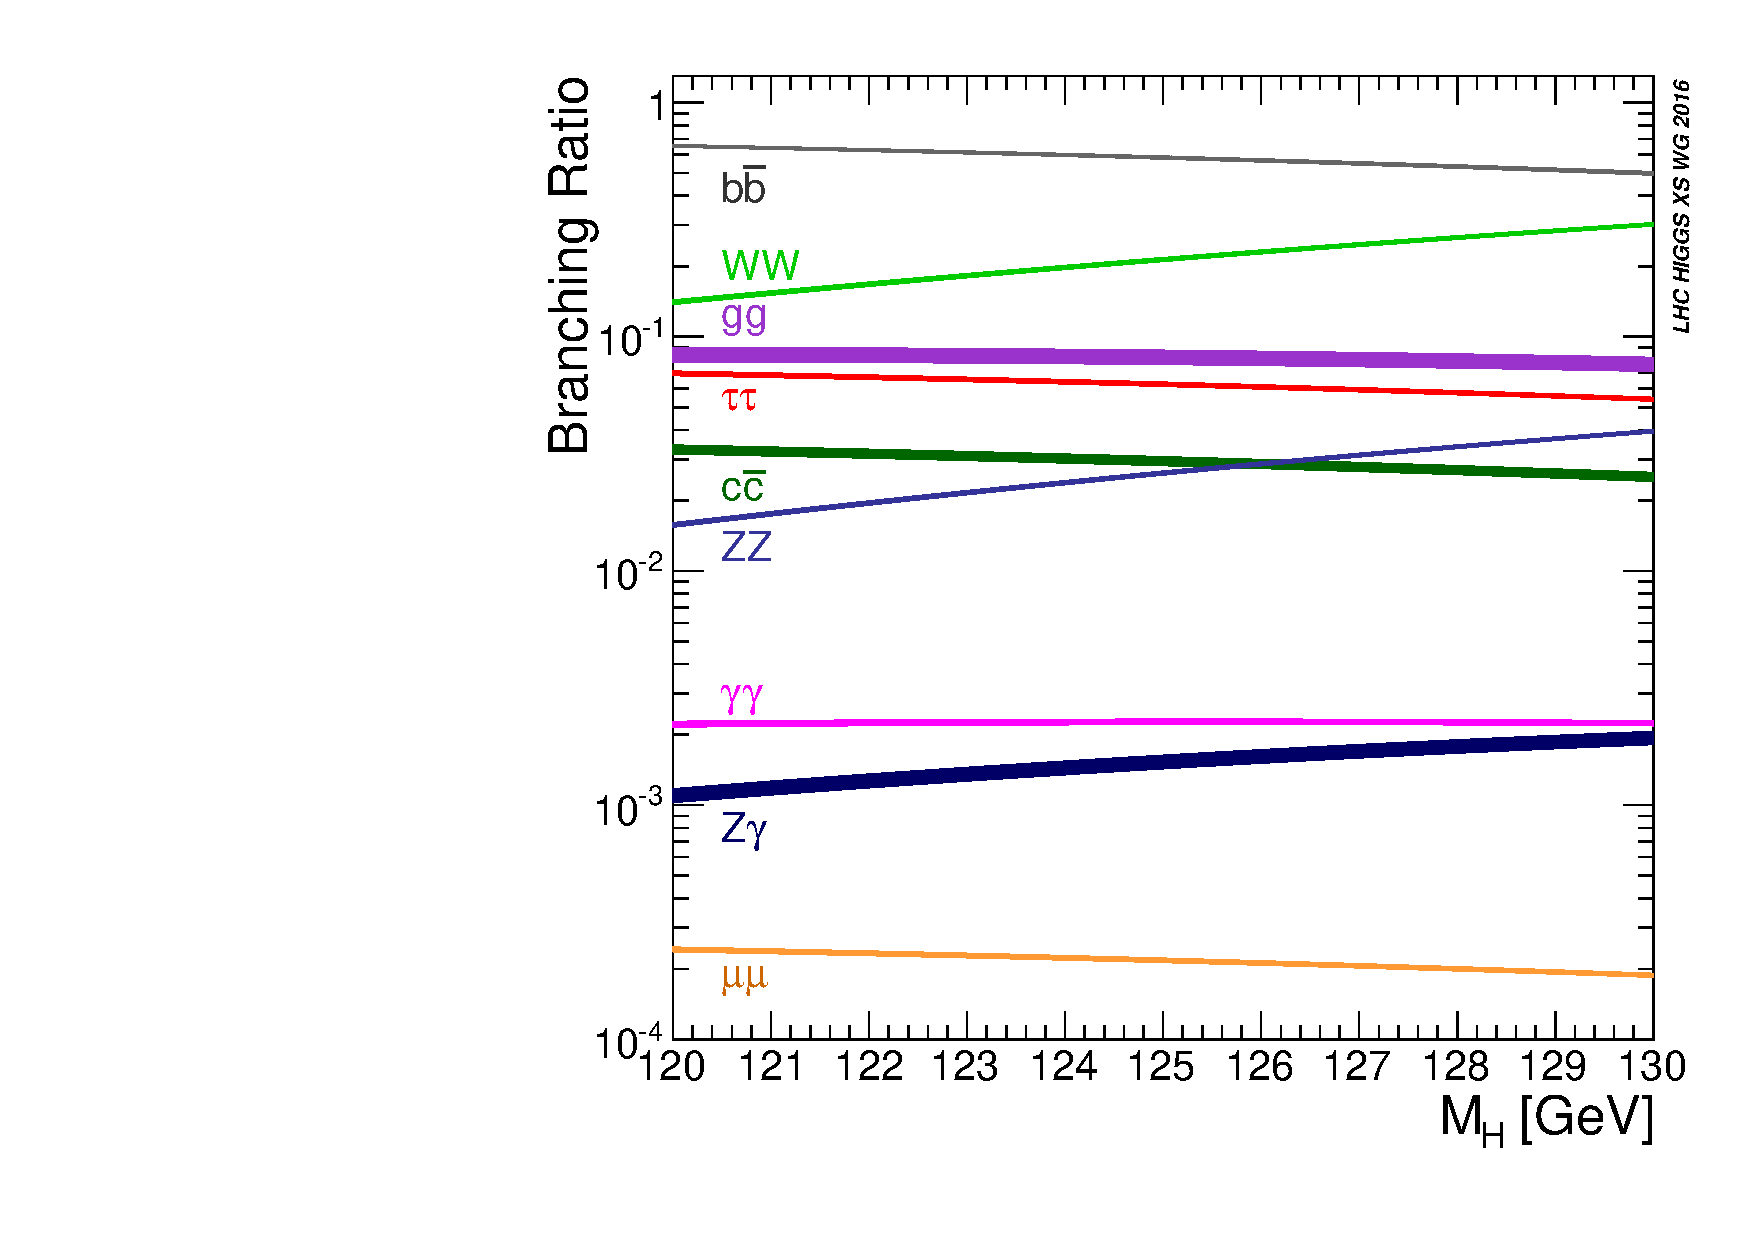
\includegraphics[width=0.49\textwidth]{figures/theory/SMHiggsBR_120-130.pdf}\label{fig:sm:h_br_theo}}
\caption{
\subref{fig:sm:h_xsec_theo} Higgs boson production cross-section at 13 TeV for a mass range between 120 and 130 GeV.
\subref{fig:sm:h_br_theo} Higgs boson \gls{br} for a mass range between 120 and 130 GeV.
Figures from Ref.  \cite{deFlorian:2016spz}.}
\label{fig:sm:h_xsec_br}
\end{figure}

The production cross-section is found to be in agreement with the \gls{sm} predictions within uncertainties. Figure \ref{fig:sm:h_xsec} shows the best fit value of Higgs production cross-section times \gls{br} in the different production and decay modes \cite{Khachatryan:2016vau}. Also the relation between the fermion or boson mass and the Higgs coupling has been verified experimentally, as show in Figure \ref{fig:sm:h_mass}. 

\begin{figure}[ht]
\centering
\subfigure[]{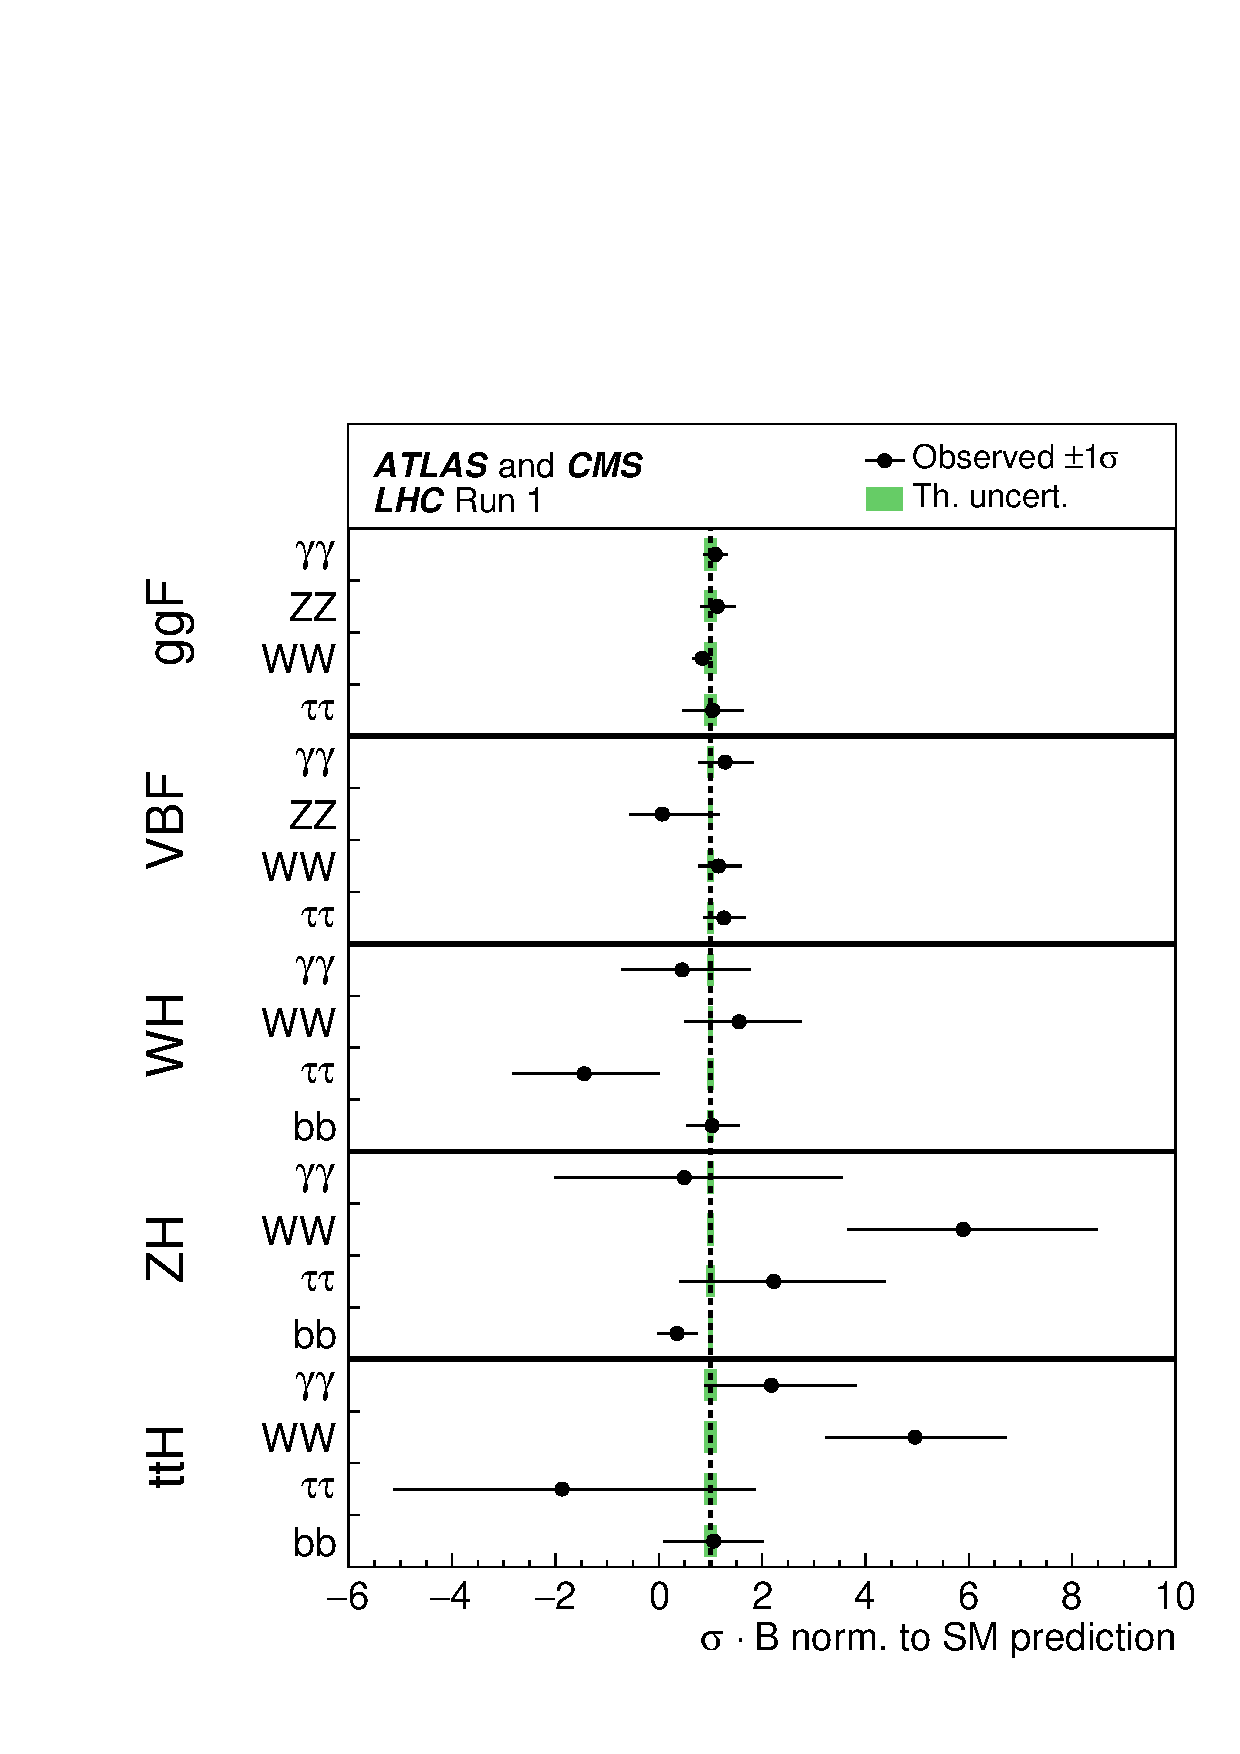
\includegraphics[width=0.49\textwidth]{figures/theory/CMS-HIG-15-002_Figure_007}\label{fig:sm:h_xsec}}
\subfigure[]{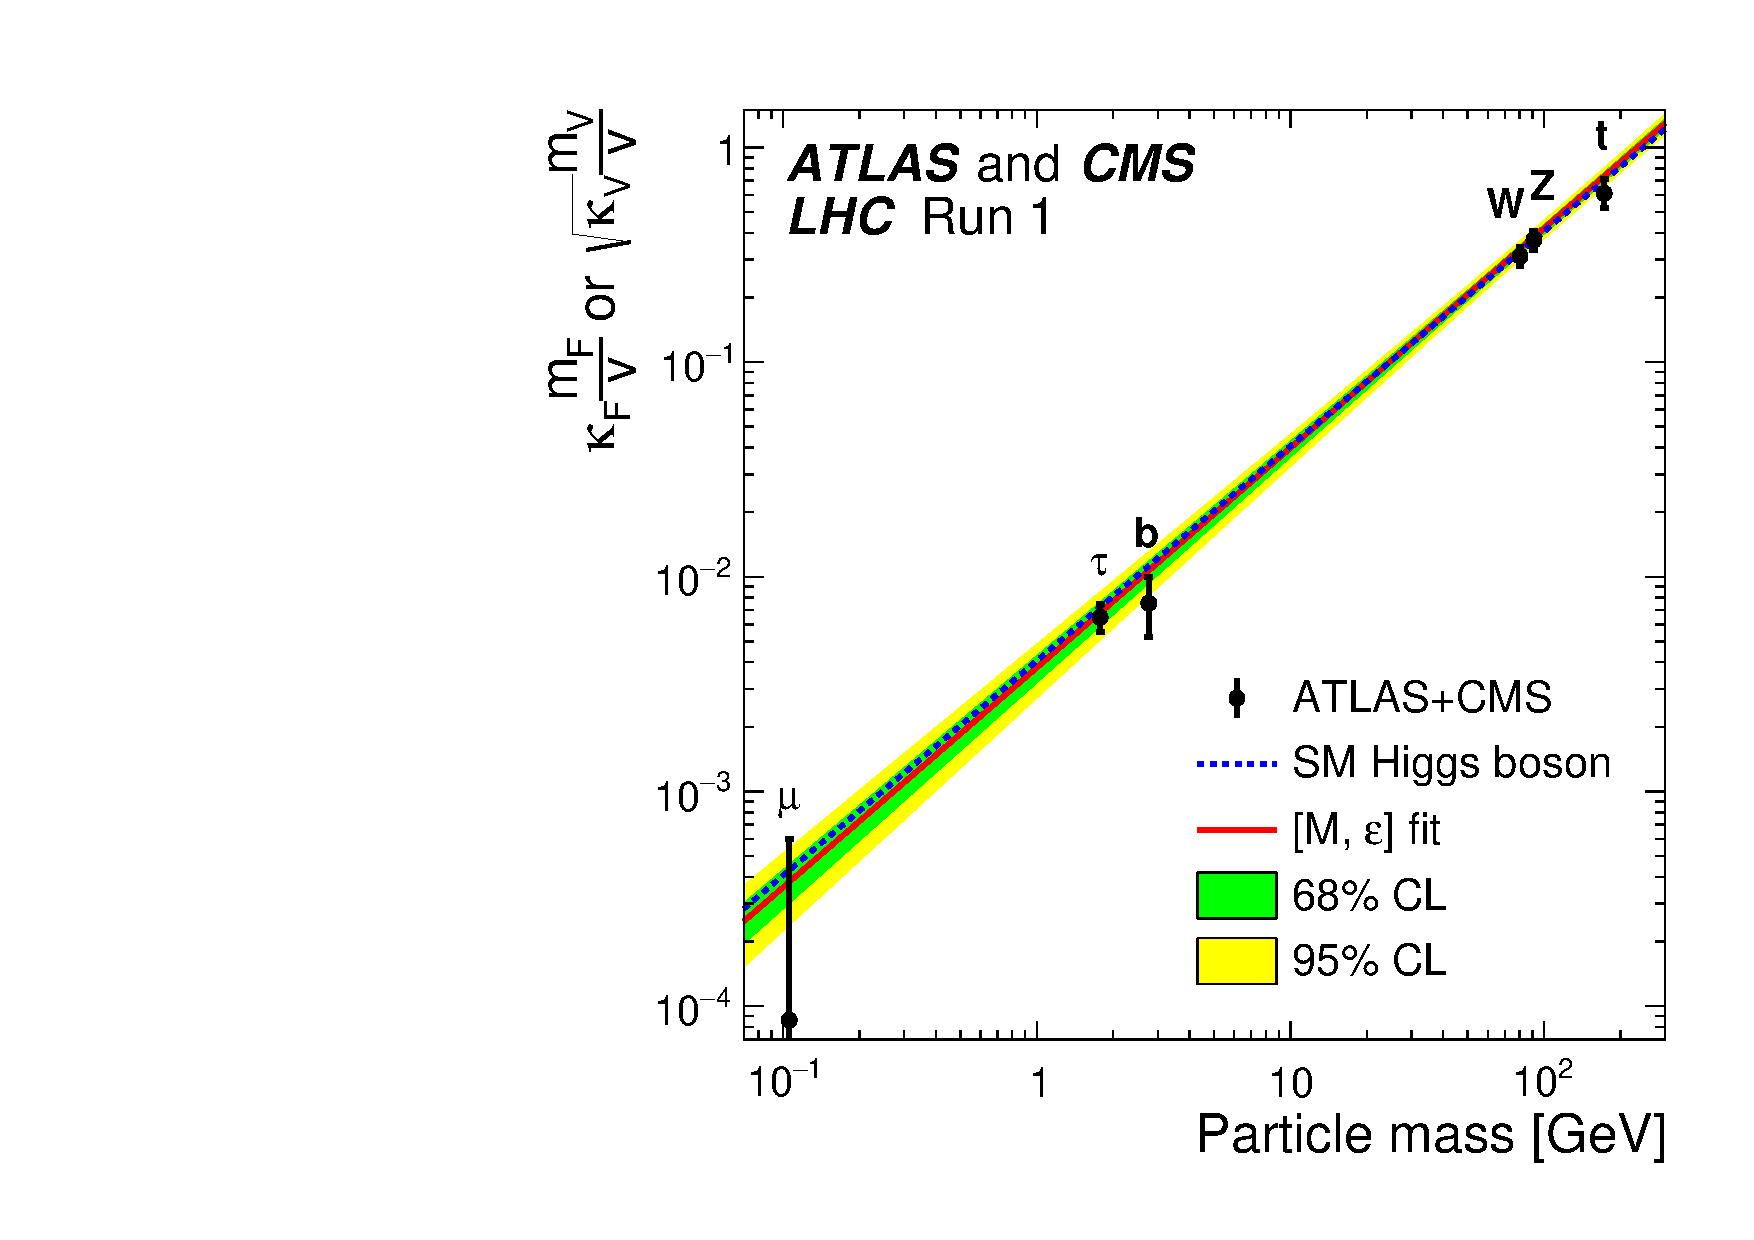
\includegraphics[width=0.49\textwidth]{figures/theory/CMS-HIG-15-002_Figure_019}\label{fig:sm:h_mass}}
\caption{\subref{fig:sm:h_mass} Best-fit values as a function of particle mass for the combination of Run 1 ATLAS and CMS data. \subref{fig:sm:h_xsec} Best-fit value of Higgs production cross-section times \gls{br} in different production and decay modes. Figure from Ref.  \cite{Khachatryan:2016vau}.}
\label{fig:sm:h_couplings_mass}
\end{figure}

 


\section{Limitations of the Standard Model and how to extend it}
\label{sec:smsusy:bsm}

Despite its undeniable success in describing the subatomic world, the \gls{sm} has some limitations that suggest it should be considered as the low-energy approximation of a more general theory. Nowadays there is no perfect candidate to fill the role of this general theory, but the shortcomings of the \gls{sm} highlight the characteristics this theory should have. Section \ref{sec:sm:missingpieces} discusses the experimental observations that are not accounted by the \gls{sm} framework, whose lacking is an objective limit of the \gls{sm}. In section \ref{sec:sm:aesthetics} we review some other features that the \gls{sm} is missing that, while not being strictly necessary, would be desirable in a general theory. Some theories and models candidate to extend the \gls{sm} are briefly presented in Section \ref{sec:sm:extensions}.

\subsection{Unexplained phenomena}
\label{sec:sm:missingpieces}

The \gls{sm} lacks an explanation for some well established experimental phenomena that are listed in the next paragraphs.

\subsubsection*{Neutrino Masses}

Neutrino oscillations \cite{PhysRevLett.81.1562} are possible only if there is a mass difference between the three neutrino generations, which automatically implies non-zero masses for at least some neutrinos. Although neutrino mass terms could be accommodated by the \gls{sm} through right-handed neutrinos or a description of neutrinos as Majorana particles, the basic formulation of the \gls{sm} describes neutrinos as massless particles.

\subsubsection*{Dark Matter and Dark Energy}

The \gls{sm} describes only baryonic matter; this accounts for about 5\% of the energy density in the universe. Even though no direct observation of it has been made so far, we know there is also another type of matter, that does not have electromagnetic interactions and  is about five times more abundant than ordinary matter.  Since this type of matter does not reflect light, it is referred to as dark matter. The presence of dark matter has been postulated for the first time from the rotational velocity of galaxies \cite{Zwicky:1937zza}, but this evidence has now been confirmed also by other observations, including the analysis of the cosmic microwave background from the WMAP and Planck collaborations \cite{Larson:2010gs,Ade:2013zuv}. The sum of baryonic and dark matter accounts for about 32\% of the of the energy density in the universe. 
The remaining 68\%, known as dark energy, is the energy responsible for the accelerated expansion of the universe. While some extensions of the \gls{sm} provide candidates for dark matter, at the moment no theory provides a compelling explanation for dark energy.


\subsubsection*{CP Violation}

CP-violating processes are needed in order to generate the observed asymmetry between the matter and the anti-matter content of our universe. While the \gls{sm} provides one source of CP violation with the complex phase in the \gls{ckm} matrix mentioned in Section \ref{sec:smsusy:ew}, this is not enough and additional sources are needed in order to explain the observed asymmetry.

\subsubsection*{Gravity}

Gravity is the only force acting on elementary particles that is not described by the \gls{sm}. In fact, not only is not described by the \gls{sm}, but the simple attempt to quantize gravity through a spin-2  mediator (graviton) leads to a non-renormalizable theory. The strength of gravity is expected to be comparable to that of the other forces at the Planck scale ($\Lambda_{Planck}$, $\approx 10^{19}$ GeV). 

\subsection{Aesthetic shortcomings}
\label{sec:sm:aesthetics}

While the previous section discusses objective shortcomings of the \gls{sm}, there are also some aesthetic criteria that the \gls{sm} does not seem to satisfy. These are mostly based on the concept of Naturalness: unless there is a good reason, the parameters of a "beautiful" theory should be all of the same order of magnitude, and a theory where instead the parameters are bound to assume very specific and different values (fine tuning) seems "unnatural". It is important to notice that this naturalness requirement is subjective, as well as the amount of fine tuning allowed for a theory to be considered natural.


\subsubsection*{Hierarchy Problem}

The expression for the mass of the Higgs boson in Equation \ref{eq:sm:Higgsmass} contains only the tree-level contribution. The proper computation should include the radiative contributions from all the particles that couple with the Higgs boson, directly or indirectly (see below). A fermion, whose Yukawa coupling leads to the interaction $-y_f \phi \bar{f} f$, will produce a correction to the Higgs boson mass with a divergent integral; this can be computed e.g. with a cut-off regularization, and in this case the resulting correction to the Higgs boson mass, shown in Figure  \ref{fig:sm:h_corr_fermion}, is:
\begin{equation}
\Delta m_H^2 \>=\>  
-{|y_f|^2\over 8 \pi^2} \Lambda_{UV}^2 + \mathcal{O}(\ln \Lambda_{UV} ) \; ,
\label{eq:divhf}
\end{equation}

\noindent where $\Lambda_{UV}^2$ is the cut-off scale, identified with the limit of validity of the theory. If we assume that no physics \gls{bsm} is present up to $\Lambda_{Planck}$, having corrections to the mass proportional to $\Lambda_{Planck}$ requires a fine tuning of the parameters of the order of $\frac{m_H}{\Lambda_{Planck}} \approx 10^{-17}$. This is due to the strong hierarchy of the scales involved (hierarchy problem) \cite{Weinberg:1975gm, PhysRevD.20.2619, PhysRevD.14.1667, tHooft:1979rat}. Since the correction to the mass is proportional to the Yukawa coupling of the fermion, it is clear that the most important correction is the one given by the top quark, whose Yukawa coupling is $y_t \approx 1$. % 0.996 

Despite this, it can still be argued that the appearance of the $\Lambda_{UV}$ divergence is connected more to the regularization scheme rather than to the theory itself. But even in this case, the value of 125 GeV for the Higgs boson mass remains difficult to justify. The \gls{sm} Lagrangian does not have any symmetry that prevents the Higgs boson to couple to new \gls{bsm} particles. If we assume the existence of a complex scalar that couples with the Higgs field through $ -y_S|\phi|^2 |S|^2$, the correction to the Higgs propagator, shown in Figure \ref{fig:sm:h_corr_scalar}, is given by:

\begin{equation}
\Delta m_H^2 \>=\> {y_S\over 16 \pi^2}
\left [\Lambda_{UV}^2 - 2 m_S^2
\> {\rm ln}(\Lambda_{UV}/m_S) + \ldots
\right ] \; .
\label{eq:divhs}
\end{equation}

\noindent Beside the first term, proportional to $\Lambda_{UV}^2$, that can be thought as a consequence of the cut-off regularization, we also have a second  term proportional to $m_S^2$. If we assume that \gls{bsm} physics exists and that, since it has not yet been observed, $m_S$ must be large, this contribution drives $m_H$ to high values. A similar argument applies even if the new \gls{bsm} sector and the Higgs field do not couple directly but, for example, share a gauge interaction.

\begin{figure}[ht]
\centering
\subfigure[]
{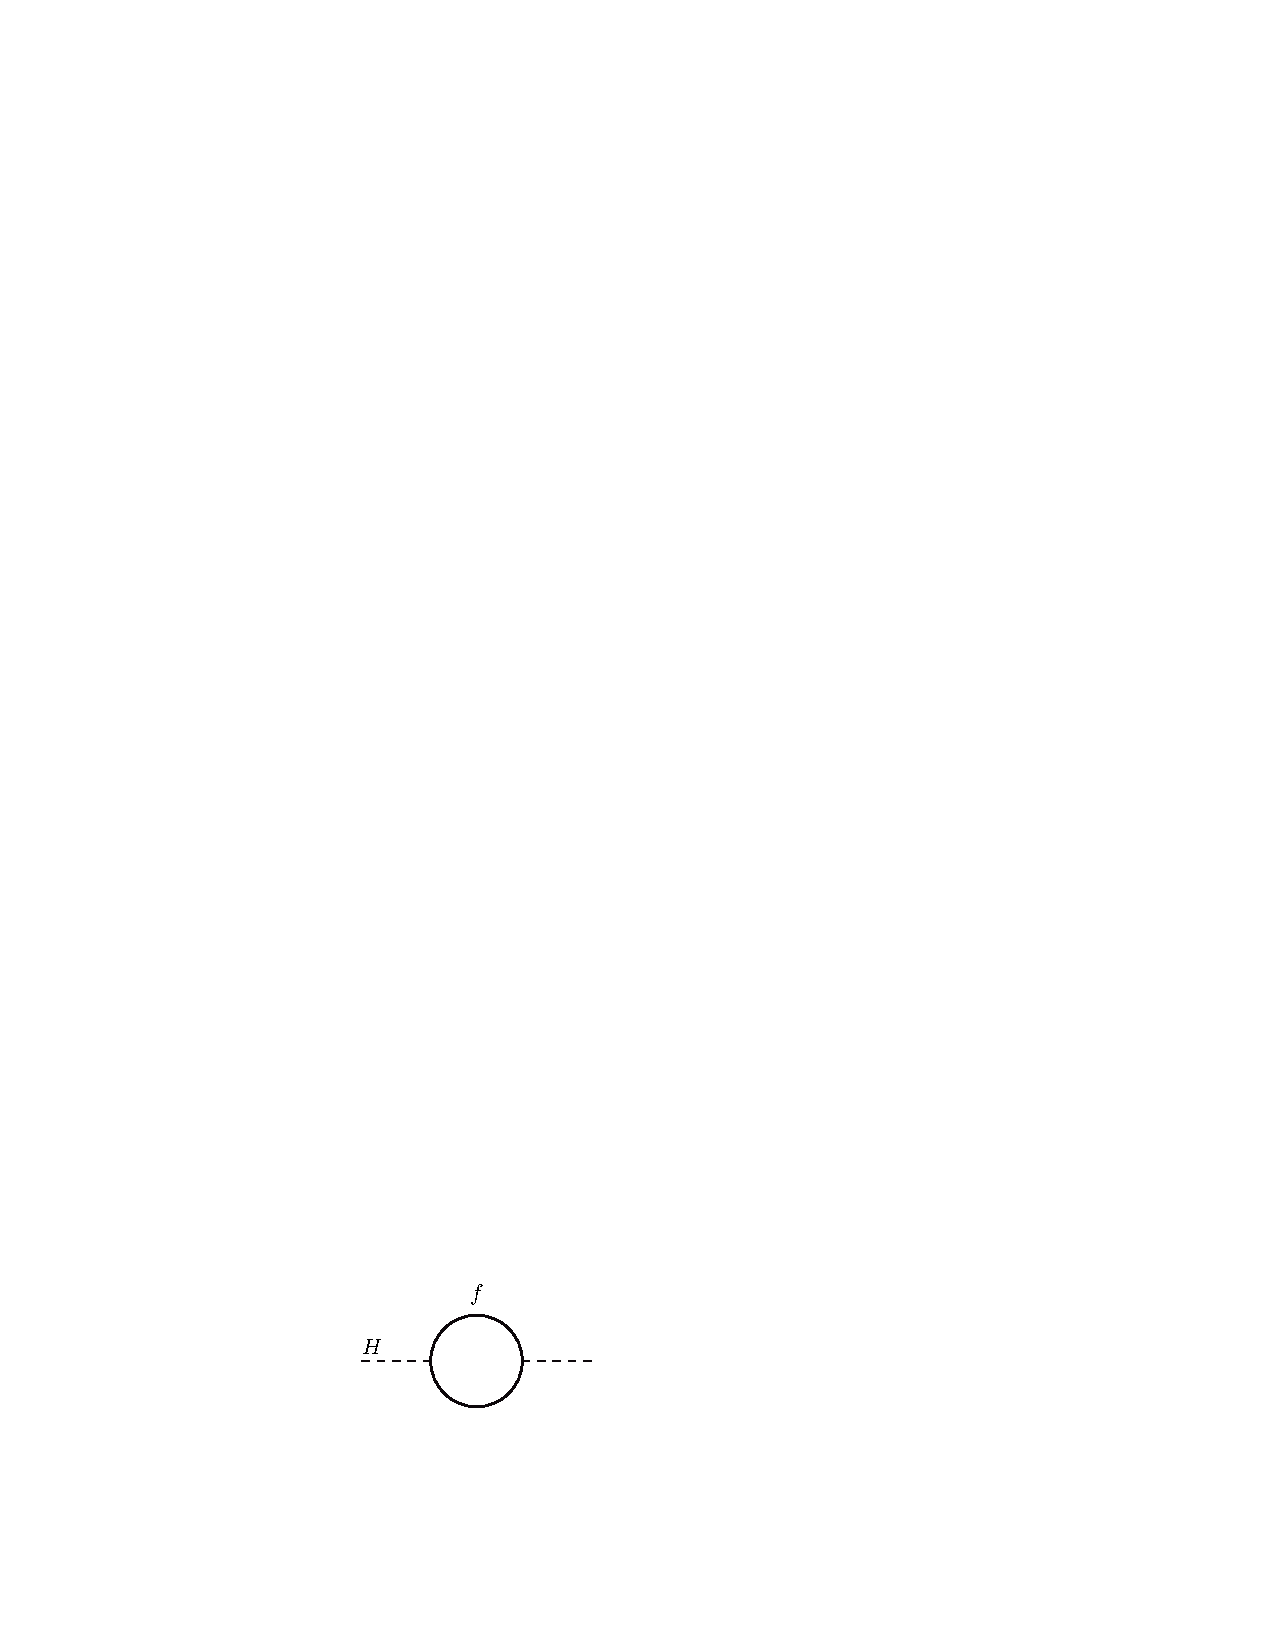
\includegraphics[width=0.36\textwidth]{figures/theory/h_corr_f.pdf}\label{fig:sm:h_corr_fermion}}
\subfigure[]{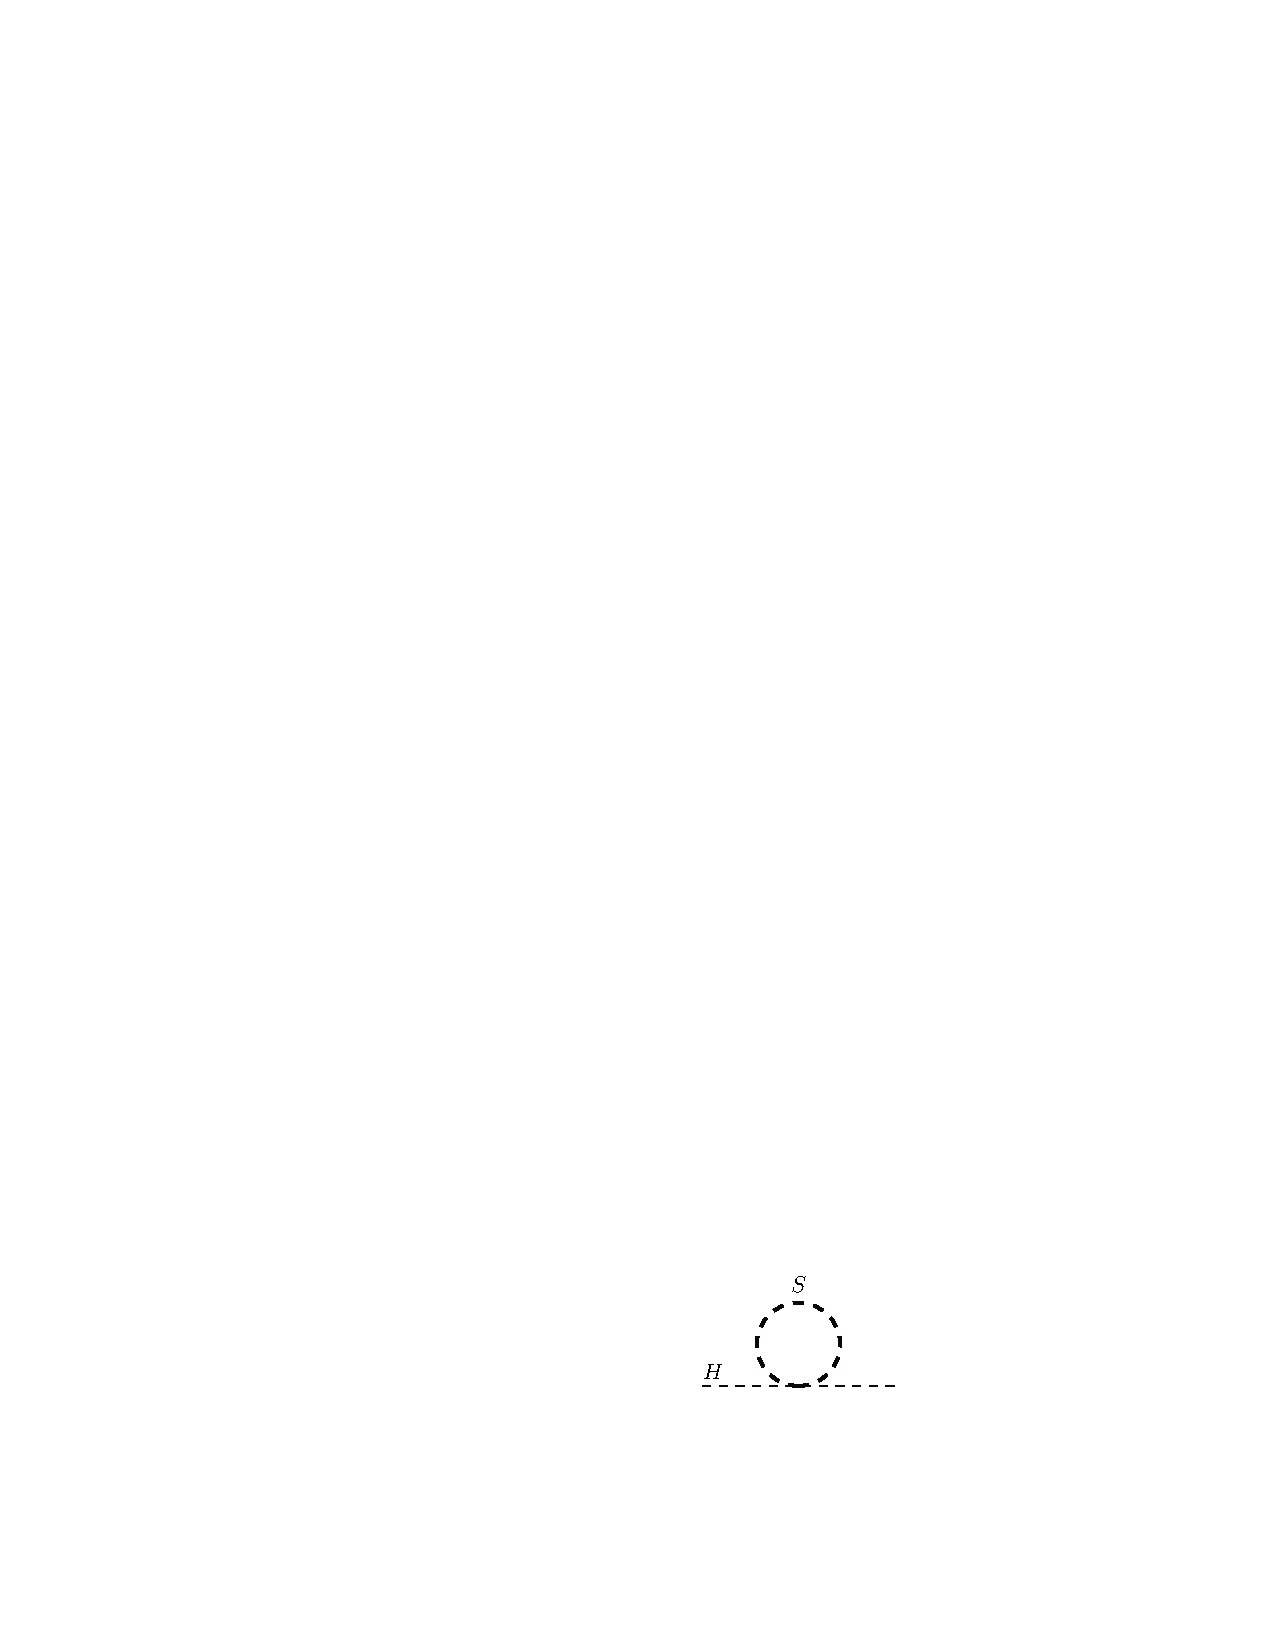
\includegraphics[width=0.36\textwidth]{figures/theory/h_corr_s.pdf}\label{fig:sm:h_corr_scalar}}
\caption{Correction to the Higgs boson propagator form the interaction with \subref{fig:sm:h_corr_fermion} a fermion and \subref{fig:sm:h_corr_scalar} a scalar. Figure from Ref. \cite{Martin:1997ns}.}
\label{fig:sm:h_corr}
\end{figure}

\subsubsection*{Fermion Mass Hierarchy} 

Fermion masses are less sensitive than the Higgs boson mass to the cut-off scale as the divergence is only logarithmic. Nevertheless, it is striking how strong the fermion Yukawa coupling hierarchy is: even if we don't consider neutrinos, fermion masses span about six orders of magnitude, without any apparent reason.

\subsubsection*{Unification of Coupling Constants}

The \gls{sm} coupling constants of the $SU(3)_\mathrm{C}$, $SU(2)_\mathrm{L}$ and $U(1)_\mathrm{Y}$ groups have a different evolution, and the extrapolation of their values at very high energies suggests a common value at a scale $M_{GUT} \approx 10^{15}-10^{16}$ GeV, after which the different couplings should unify. However, if the only particles involved in the computation of the evolution of the coupling constants are the \gls{sm} ones, there is no exact crossing point, as shown in Figure \ref{fig:susy:gut_0}.

\subsection*{Strong CP Problem}

The most general \gls{sm} \gls{qcd} Lagrangian should include also a CP-violating angle, and this would not spoil renormalizability. The presence of this term would have directly measurable physical consequences, for example a non-zero electric dipole moment for the neutron (nEDM). The tight  limits on the nEDM ( $< 3.6 \times 10^{-26}$ e cm at 95\% CL \cite{PhysRevD.92.092003}) translate into upper limits on the parameter regulating the CP-violating term of the \gls{qcd} Lagrangian ($\theta < 10^{-10}$ rad), while there is no theoretical reason why it should not be of order 1. 


\subsection{Extensions of the Standard Model}
\label{sec:sm:extensions}

The aspects of the particle physics world not yet described by the \gls{sm}, are an indication that the \gls{sm} should be extended.
In this section we briefly discuss a few of the most popular models proposed to extend the \gls{sm}, except from Supersymmetry which is discussed in more details in Section \ref{sec:smsusy:susy}. These extensions introduce typically one or more of the following:

\begin{itemize}
\item New particles, that can either be independent particles or "partners" of the \gls{sm} particles.
\item New symmetries, that can be broken. 
\item New degrees of freedom, such as new quantum numbers or extra dimensions.
\item New forces, whose strength depends on the energy scale.
\end{itemize}

\subsubsection*{Little Higgs}
% chiara: expand
Little Higgs models address the problem of the Higgs boson mass by considering the Higgs boson as a pseudo-Goldstone boson of a global symmetry \cite{PhysRevD.12.508, Kaplan:1983fs, KAPLAN1984187, DUGAN1985299}. This leads to a light mass for the Higgs boson is a similar way as for the pion in \gls{qcd}.

\subsubsection*{Technicolor}
In technicolor models \cite{Weinberg:1975gm, PhysRevD.20.2619} the mass of the $Z$ and $W^{\pm}$ bosons is not generated through the interaction with the Higgs boson, but dynamically with a new asymptotically free gauge interaction whose strength is higher at small distances; the analogy with \gls{qcd} (and the "color" degree of freedom) leads to the name technicolor. New fermions ("technifermions") are also introduced, transforming under the group vectorial representation. The Higgs boson is not predicted by technicolor, but it can be included in the model as a singlet scalar resonance, a dilaton, or a singlet pseudo-Goldstone boson.

\subsubsection*{Extra Dimensions}

The first attempt to introduce additional spacial dimensions to unify forces was done in the 1920's by Kaluza and Klein \cite{Kaluza, Klein:1926tv}, who interpreted our four-dimensional universe as a "brane" of a higher-dimensional space-time. While the \gls{sm} foresees only three spatial dimensions, adding extra dimensions can explain the observed weakness of gravity with respect to the other forces as it would be diluted in the extra dimensions. 
% rephrase
Particles propagating in the extra dimensions manifest in our brane as Kaluza-Klein modes. % end rephrase
While the original model from Kaluza and Klein was disproved shortly shortly after being proposed, similar ideas and formalism have also been used afterwards:  

\begin{itemize}
\item In the Arkani-Hamed-Dimopoulos-Dvali (ADD) model \cite{ArkaniHamed:1998rs}, two (or more) flat extra dimensions are added in which only gravity can propagate (through a graviton).
\item In the Randall and Sundrum model \cite{PhysRevLett.83.3370} the universe is conceived as a five-dimensional Anti-de Sitter space-time, and the weakness of gravity is explained through the red-shift of the gravity brane.
\end{itemize}


\section{Supersymmetry}
\label{sec:smsusy:susy}

\gls{susy} \cite{Wess:1974tw, Salam:1974ig} is an extension of the Poincar\'e group that rotates bosonic states into fermionic ones and vice versa, through the supercharge operator ($Q$) that carries itself a fermionic charge: 

\begin{equation}
\begin{aligned}
&Q |{\rm boson}\rangle = |{\rm fermion }\rangle \;, \\
&Q |{\rm fermion}\rangle = |{\rm boson }\rangle \; .
\end{aligned}
\end{equation}

\noindent The Haag-Lopuszanski-Sohnius extension of the Coleman-Mandula theorem \cite{HAAG1975257} allows such operator as the only non-trivial extension of the Poincar\'e group in a consistent four-dimensional theory, if the operator and his hermitian conjugate ($Q^\dagger$) satisfy the following relations:

\begin{equation}
\begin{aligned}
&\{ Q, Q^\dagger \} = P^\mu \; ,  \\
&\{ Q,Q \} = \{ Q^\dagger , Q^\dagger \} = 0  \;,  \\
&[ P^\mu , Q  ] = [P^\mu, Q^\dagger ] = 0 \; ,
\label{eq:susyalgth}
\end{aligned}
\end{equation}

\noindent where $P$ is the four-momentum operator. These relations, which define the Supersymmetry algebra, make it clear how the action of the supercharge is related to the Poincar\'e group: the combination of two Supersymmetry rotations is a space-time translation.

\subsection{Supermultiplets}

The irreducible representations of the \gls{susy} algebra are the supermultiplets, that contain both bosons and fermions. 
\gls{susy} particles are referred to as superpartners of the \gls{sm} particles within the same supermultiplet.
Superpartners of the \gls{sm} particles are indicated with the same symbol but with a $\sim$ on top of it. Depending on their particle content, supermultiplets are classified in different categories:

\begin{description}
\item[Chiral supermultiplets] These supermultiplets are the ones containing the \gls{sm} fermions and their superpartners. Each Dirac fermionic field can be regarded as two separate Weyl field, each of which has two degrees of freedom and is associated with a complex scalar as a superpartner. The name given to superpartners of fermions is sfermions (e.g. the superpartner of the top is the stop and the superpartner of the bottom is the sbottom). Since chiral supermultiplets are formed by spin-0 and spin-$\frac{1}{2}$ particles, they contain also the \gls{susy} extended Higgs sector, as described in Section \ref{sec:susy:Higgs}.

\item[Gauge supermultiplets] Gauge bosons and their superpartners belong to gauge supermultiplets. Each spin-1 \gls{sm} boson is associated to a spin-$\frac{1}{2}$ Weyl fermion, as before the electroweak symmetry breaking all the gauge bosons are massless and have only two degrees of freedom. The name of the superpartners of the gauge bosons is the same as the corresponding \gls{sm} particle but with a -ino suffix (e.g. the gluon superpartner is the gluino). 

\item[Gravitational supermultiplets] If we assume that gravity is mediated by the graviton, then a third type of supermultiplet is necessary that contains the spin-2 graviton and its superpartner, the spin-$\frac{3}{2}$ gravitino.

\end{description}

% Avoid fine tuning

% \gls{susy} is a broken symmetry


\subsection{Minimal Supersymmetric Standard Model}
\label{sec:theo:mssm}

\gls{susy} is a framework that allows to generate an infinite number of models. The \gls{mssm} is the one that allows to include and extend the \gls{sm} with the smallest number of extra parameters, and is based on the superpotential:

\begin{equation}
\begin{aligned}
W_{MSSM} & = y_u \stilde{u} \stilde{Q} H_u - y_d \stilde{d}\stilde{Q} H_d - y_e \stilde{e} \stilde{L}H_d + \mu H_u H_d \\  
& = \sum_{F, G, T} y_u^{FG} \stilde{u}_F \stilde{Q}_G^T H_u^T -
 = \sum_{F, G, T} y_u^{FG} \stilde{u}_F \stilde{Q}_G^T H_u^T - 
   \sum_{F, G, T} y_d^{FG} \stilde{d}_F \stilde{Q}_G^T H_d^T   \\ 
   & -
   \sum_{F, G, T} y_e^{FG} \stilde{e}_F\stilde{L}_G^T H_d^T  +
   \sum_{T} \mu H_u^T H_d^T \;.
\end{aligned}
\label{eq:WMMS}
\end{equation}

\noindent The superpotential appears in the \gls{mssm} Lagrangian through first and second order derivatives as discussed e.g. in Ref. \cite{Martin:1997ns}.

\begin{table}[t]
\begin{center}
\begin{tabular}{c c c c c}
\hline
\multicolumn{2}{c}{Names} 
& Spin 0 & Spin 1/2 & $SU(3)_C ,\, SU(2)_L ,\, U(1)_Y$
\\  \hline\hline
squarks, quarks & $Q$ & $({\stilde{u}}_L\>\>\>{\stilde{d}}_L )$&
 $(u_L\>\>\>d_L)$ & $(\>{\bf 3},\>{\bf 2}\>,\>{1\over 6})$
\\
($\times 3$ families) & $\bar{u}$
&${\stilde{u}}^*_R$ & $u^\dagger_R$ & 
$(\>{\bf \overline 3},\> {\bf 1},\> -{2\over 3})$
\\ & $\bar{d}$ &${\stilde{d}}^*_R$ & $d^\dagger_R$ & 
$(\>{\bf \overline 3},\> {\bf 1},\> {1\over 3})$
\\  \hline
sleptons, leptons & $L$ &$({\stilde{\nu}}\>\>{\stilde{e}}_L )$&
 $(\nu\>\>\>e_L)$ & $(\>{\bf 1},\>{\bf 2}\>,\>-{1\over 2})$
\\
($\times 3$ families) & $\bar{e}$
&${\stilde{e}}^*_R$ & $e^\dagger_R$ & $(\>{\bf 1},\> {\bf 1},\>1)$
\\  \hline
Higgs, higgsinos &$H_u$ &$(H_u^+\>\>\>H_u^0 )$&
$(\stilde{H}_u^+ \>\>\> \stilde{H}_u^0)$& 
$(\>{\bf 1},\>{\bf 2}\>,\>+{1\over 2})$
\\ &$H_d$ & $(H_d^0 \>\>\> H_d^-)$ & $(\stilde{H}_d^0 \>\>\> \stilde{H}_d^-)$& 
$(\>{\bf 1},\>{\bf 2}\>,\>-{1\over 2})$
\\  \hline
\end{tabular}
\caption{Chiral supermultiplets in the Minimal Supersymmetric Standard Model.
The spin-$0$ fields are complex scalars, and the spin-$1/2$ fields are 
left-handed two-component Weyl fermions. Table from Ref. \cite{Martin:1997ns}. \label{tab:chiral}}
\vspace{-0.6cm}
\end{center}
\par\bigskip
\begin{center}
\begin{tabular}{c c c c}
\hline
Names & Spin 1/2 & Spin 1 & $SU(3)_C, \> SU(2)_L,\> U(1)_Y$\\
\hline\hline
gluino, gluon &$ \stilde{g}$& $g$ & $(\>{\bf 8},\>{\bf 1}\>,\> 0)$
\\
\hline
winos, W bosons & $ \stilde {W}^\pm\>\>\> \stilde {W}^0 $&
 $W^\pm\>\>\> W^0$ & $(\>{\bf 1},\>{\bf 3}\>,\> 0)$
\\
\hline
bino, B boson &$\stilde{B}^0$&
 $B^0$ & $(\>{\bf 1},\>{\bf 1}\>,\> 0)$
\\
\hline
\end{tabular}
\caption{Gauge supermultiplets in
the Minimal Supersymmetric Standard Model. Table from Ref. \cite{Martin:1997ns}. \label{tab:gauge}}
\vspace{-0.45cm}
\end{center}
\end{table}

The chiral supermultiplets of the \gls{mssm} are described in Table \ref{tab:chiral}, and the gauge supermultiples in Table \ref{tab:gauge}. Note that the states defined in these tables are interaction eigenstates, but not necessary mass eigenstates as mixing is possible. In particular, the higgsinos mix with the gauginos to form neutralinos ($\stilde{\chi}^0_i$) and charginos ($\stilde{\chi}^\pm_i$). In addition, the sfermions associated with the left and right component of the same \gls{sm} fermion mix to form the sfermion mass eigenstates (e.g. $\stilde{t}_L$ and $\stilde{t}_R$ mix to form $\stilde{t}_1$ and $\stilde{t}_2$). The gluinos instead do not undergo any mixing, as there are no other superpartners with the same  quantum numbers. The gauge mass eigenstates of the \gls{mssm} are listed in Table \ref{tab:undiscovered}, assuming that the mixing within the first- and second-generation sfermions is negligible.


\begin{table}[tb]
\begin{center}
\begin{tabular}{c c c c c }
\hline
Names & Spin & $P_R$ & Gauge Eigenstates & Mass Eigenstates \\
\hline\hline
Higgs bosons & 0 & $+1$ & 
$H_u^0\>\> H_d^0\>\> H_u^+ \>\> H_d^-$ 
& 
$h^0\>\> H^0\>\> A^0 \>\> H^\pm$
\\ \hline
& & &${\stilde u}_L\>\> {\stilde u}_R\>\> \stilde d_L\>\> \stilde d_R$&(same)
\\
squarks& 0&$-1$& ${\stilde s}_L\>\> {\stilde s}_R\>\> \stilde c_L\>\>
\stilde c_R$& (same) \\
& & &
$\stilde t_L \>\>\stilde t_R \>\>\stilde b_L\>\> \stilde b_R$ 
&
${\stilde t}_1\>\> {\stilde t}_2\>\> \stilde b_1\>\> \stilde b_2$
\\ \hline
& & &${\stilde e}_L\>\> {\stilde e}_R \>\>\stilde \nu_e$&(same) 
\\
sleptons& 0&$-1$&${\stilde \mu}_L\>\>{\stilde \mu}_R\>\>\stilde\nu_\mu$&(same)
\\
& & &
$\stilde \tau_L\>\> \stilde \tau_R \>\>\stilde \nu_\tau$ 
&
${\stilde \tau}_1 \>\>{\stilde \tau}_2 \>\>\stilde \nu_\tau$
\\
\hline
neutralinos & $1/2$&$-1$ & 
$\stilde B^0 \>\>\>\stilde W^0\>\>\> \stilde H_u^0\>\>\> \stilde H_d^0$   
&
$\stilde \chi^0_1\>\> \stilde \chi^0_2 \>\>\stilde \chi^0_3\>\> \stilde \chi^0_4$ 
\\
\hline
charginos & $1/2$&$-1$ & 
$\stilde W^\pm\>\>\> \stilde H_u^+ \>\>\>\stilde H_d^-$ 
&
$\stilde \chi_1^\pm\>\>\>\stilde \chi_2^\pm $ 
\\
\hline
gluino & $1/2$&$-1$ &$\stilde g$  &(same) \\
\hline
${\rm goldstino}\atop{\rm (gravitino)}$ & ${1/2}\atop{(3/2)}$&$-1$&$\stilde 
G$  &(same) \\
\hline
\end{tabular}
\caption{The gauge and mass eigenstates of the \gls{mssm}. Table from Ref. \cite{Martin:1997ns}. 
\label{tab:undiscovered}}
\vspace{-0.4cm}
\end{center}
\end{table}%

Once the \gls{mssm} particles are introduced the computation of the evolution of the coupling constants, the unification of the forces discussed in Section \ref{sec:sm:aesthetics} is achieved, as shown in Figure \ref{fig:susy:gut_1}.

% Unifications of the coupling constants
\begin{figure}[ht]
\centering
\subfigure[]{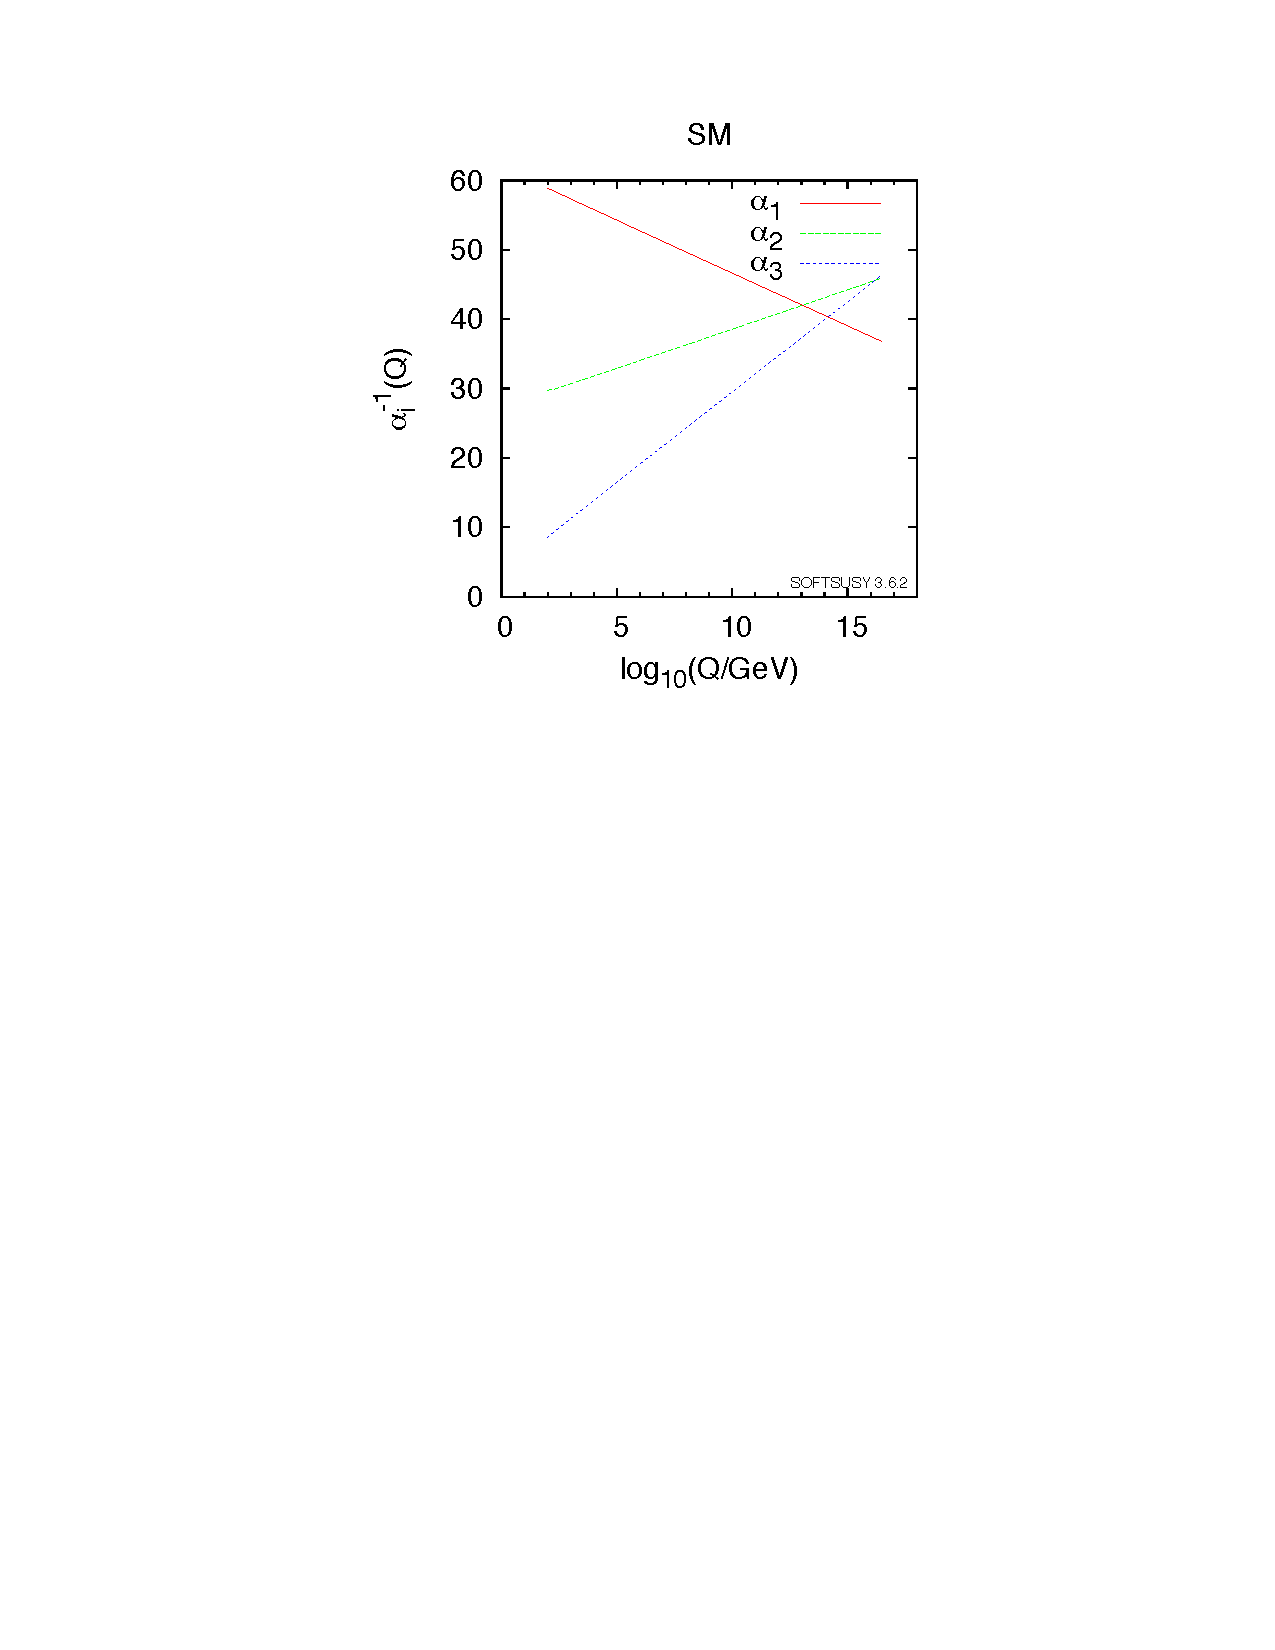
\includegraphics[width=0.49\textwidth]{figures/theory/gut_0.pdf}\label{fig:susy:gut_0}}
\subfigure[]{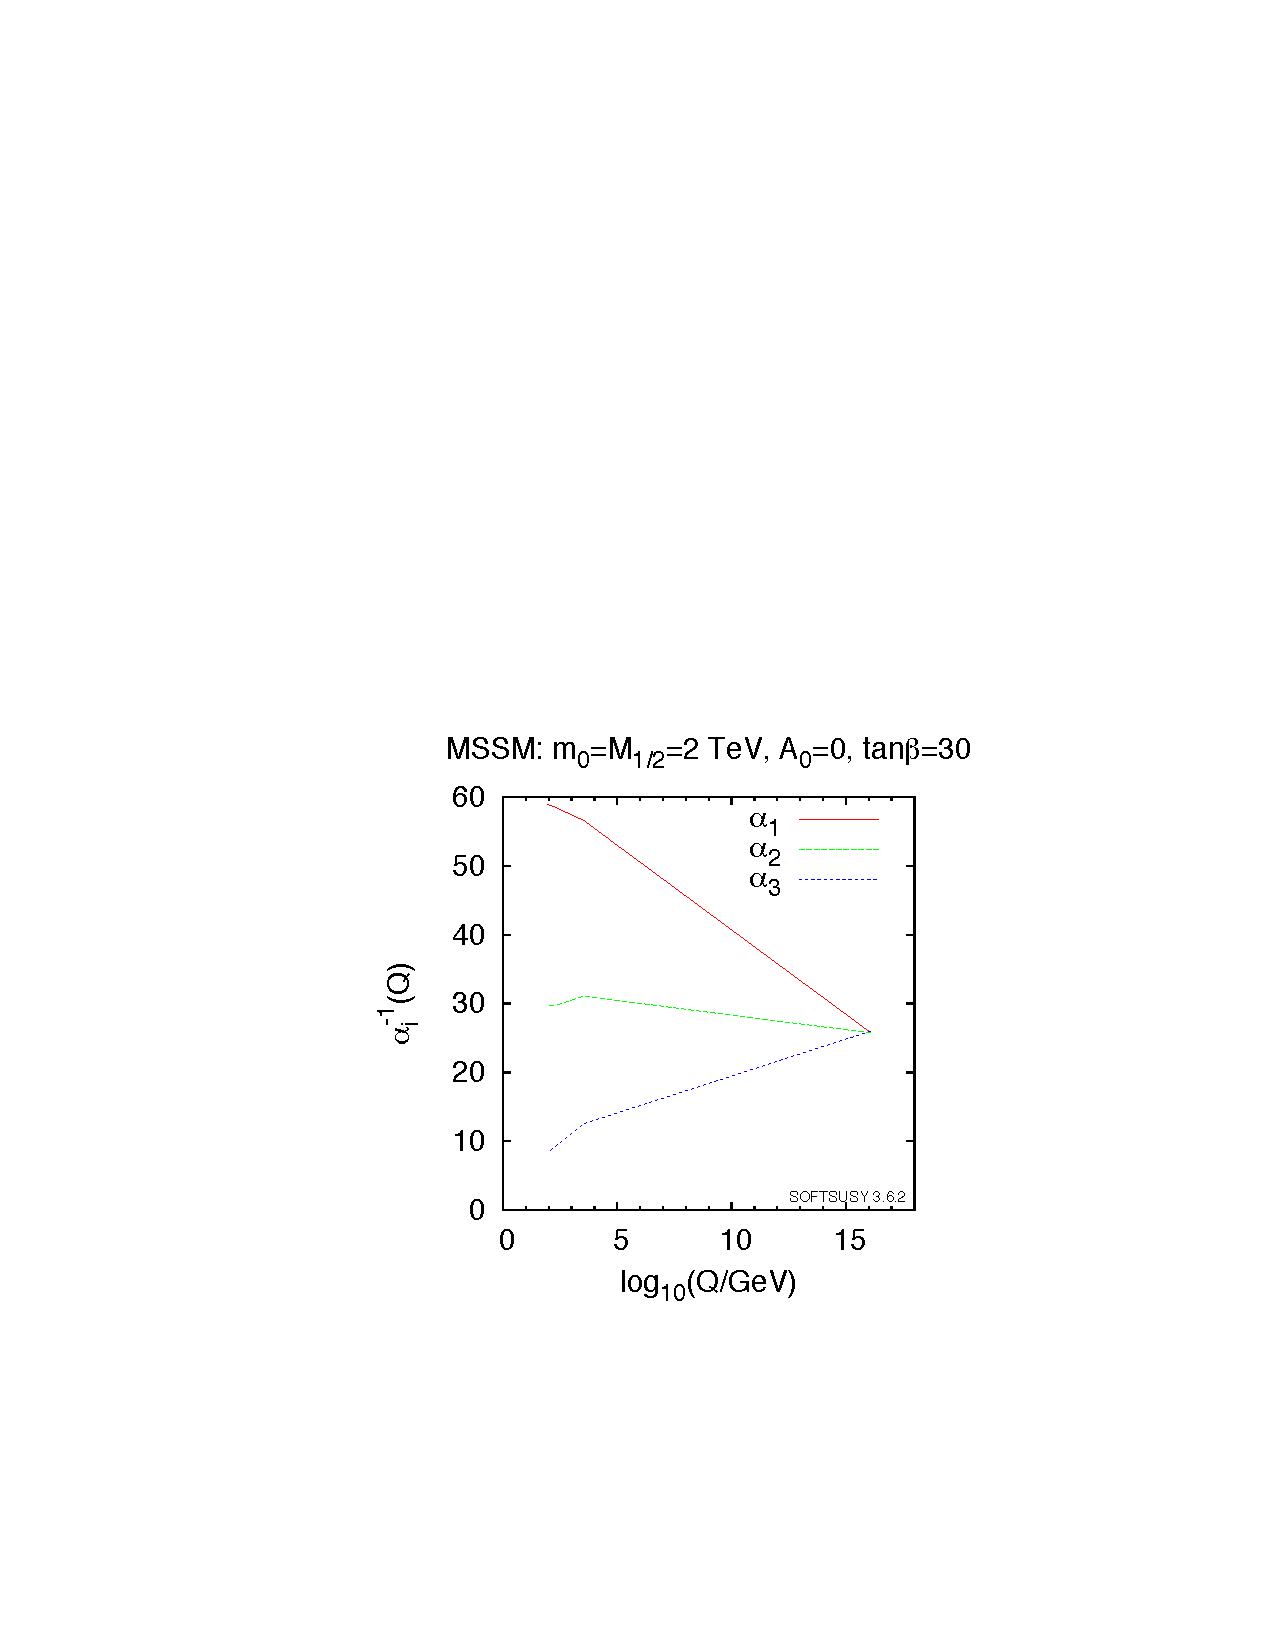
\includegraphics[width=0.49\textwidth]{figures/theory/gut_1.pdf}\label{fig:susy:gut_1}}
\caption{Evolution of the gauge couplings with energy scale in \subref{fig:susy:gut_0} the \gls{sm} and \subref{fig:susy:gut_1} the \gls{mssm}. Figure from Ref. \cite{Patrignani:2016xqp}.}
\label{fig:susy:gut}
\end{figure}

\subsubsection*{MSSM Higgs Sector}
\label{sec:susy:Higgs}

To maintain an holomorphic superpotential, \gls{susy} requires at least two SU(2) doublets: one to give mass to up-type quarks ($H_u$) and one to give mass to the the down-type quarks ($H_d$). The two doublets provide eight degrees of freedom. Three of them are  needed to give masses to the gauge bosons, while the other five become observable particles:
\begin{itemize}
\item Two CP-even neutral Higgs bosons: $h^0$ (the lighter) and $H^0$.
\item $A^0$, a CP-odd Higgs boson.
\item Two charged Higgs bosons, $H^+$ and $H^-$.
\end{itemize}


\subsubsection*{R-parity}

The \gls{mssm} does not include all the possible terms that are gauge- and \gls{susy}-invariant, to avoid interactions that would violate lepton or baryon number conservation. Matter parity, defined as:

\begin{equation}
P_M = (-1)^{3 (B-L)} \; ,
\label{eq:defmatterparity}
\end{equation}

\noindent is a multiplicative quantum number whose conservation implies automatically the conservation of lepton and baryon numbers (denoted with $L$ and $B$ respectively), without having to impose their conservation by hand. Particles in the same supermultiplet have the same matter parity: $P_M =-1$ for lepton and quark supermultiplets, while the Higgs and gauge supermultiplets have $P_M =+1$.

A more convenient way to express the same conservation rule is R-parity:

\begin{equation}
P_R = (-1)^{3(B-L) + 2 s} \; ,
\label{eq:defRparity}
\end{equation}

\noindent where $s$ is the spin of the particle. This is equivalent to matter parity as $(-1)^{2s}$ is conserved in all interactions where angular momentum conservation holds. The advantage of R-parity over matter parity is that for all \gls{sm} particles $P_R = 1$ and for all \gls{susy} particles $P_R=-1$. If  R-parity is conserved, in a collider experiment \gls{susy} particles are always produced in pairs, and each \gls{susy} particle always has an odd number of \gls{susy} particles in its decay products. As a consequence, the \gls{lsp} is stable; if the \gls{lsp} is electrically neutral, it interacts with ordinary matter mainly through gravity and thus it provides a good candidate for dark matter.

Note that R-parity conservation is not deduced from the theory and thus, while its consequences are appealing (especially the provision of a dark matter candidate), it is not an assumption that holds in all \gls{susy} models.



\subsection{Natural SUSY}
\label{sec:theo:naturalsusy}

Particles within the same supermultiplet share the same electric charge, isospin and \gls{qcd} color as $Q$ and $Q^\dagger$ commute with the generator of the gauge transformations.
The third equality in Equation \ref{eq:susyalgth} implies that $[ (P^\mu)^2 , Q  ]=0$. If we think of this as an operator applied to a supermultiplet, this implies that all the particles within the same supermultiplet should also have the same mass. The superpartners also bring a radiative correction to the Higgs boson mass, since they couple to the Higgs boson with the same coupling constant as their \gls{sm} partners ($y_S=y_f=y$). If we consider the case of a fermion and a sfermion, according to Eqs. \ref{eq:divhf}-\ref{eq:divhs} the two contributions have opposite sign and the total correction is:

\begin{equation}
\Delta m_H^2 \>=\> {y\over 16 \pi^2}
\left [ m_f^2
\> {\rm ln}(\Lambda_{UV}/m_f) 
- m_S^2
\> {\rm ln}(\Lambda_{UV}/m_S) 
\right ].
\label{eq:divhsusy}
\end{equation}

This correction cancels if each \gls{sm} particle and its superpartner have the same mass. Unfortunately we know that, if \gls{susy} exists, it must be a broken symmetry as the superpartners do not have the same mass as the corresponding \gls{sm} particles (otherwise they would have been already observed). Since the correction to the Higgs boson mass becomes larger with the increase of the mass difference between particles in the same supermultiplet, \gls{susy} remains a solution to the hierarchy problem as long as this mass difference is reasonably small. The term natural \gls{susy} refers to the class of \gls{susy} models that allow to solve (or mitigate) the fine-tuning problem that affects the Higgs boson mass; this has been a very active topic of discussion both before the start of the \gls{lhc} (see e.g. Refs. \cite{BARBIERI198863, Dimopoulos:1995mi}) and after (e.g. Refs. \cite{Papucci:2011wy, Casas:2014eca}) 

Not all the superpartners have the same relevance in the contribution to the Higgs-mass corrections, and a \gls{susy} model can be natural even if  most particles in it are extremely heavy. The particles that should be light in a natural \gls{susy} model are summarized in Figure  \ref{fig:NaturalSpectrum} and are:
\begin{itemize}
\item higgsinos, whose tree-level mass is directly controlled by the $\mu$ parameter,
\item Stops, which contribute at one loop to the Higgs boson mass, and
\item Gluinos, which contribute at two loops, since they give a one-loop correction to the stop mass.
\end{itemize}

% formula for relation between mass difference and correction to Higgs boson mass

%In the MSSM, the mass of the $Z$ boson and the Higgs sector masses are related at tree level through:
%\begin{equation}
%\label{eq:tune}
%-\frac{m_Z^2}{2} = |\mu|^2 + m_{H_u}^2.
%\end{equation}
%Where $\mu$ is the higgsino mass parameter and $m_{H_u}$ the mass term for the Higgs field that gives mass to down-type quarks. While \ref{eq:tune} holds only at tree level, it still means that if the masses of the superpartners in the Higgs sector are too large, fine-tuned loop corrections will be required to bring the left side of the equation down to the observed value of the $Z$-boson mass.

%\begin{equation}
%\Delta \equiv \frac{2\delta m_{H}^{2}}{m_{h}^{2}}.
%\end{equation}
% Z mass at tree level and definition of fine tuning

% susy particles that have to be light 

\begin{figure}[h!]
\begin{center} 
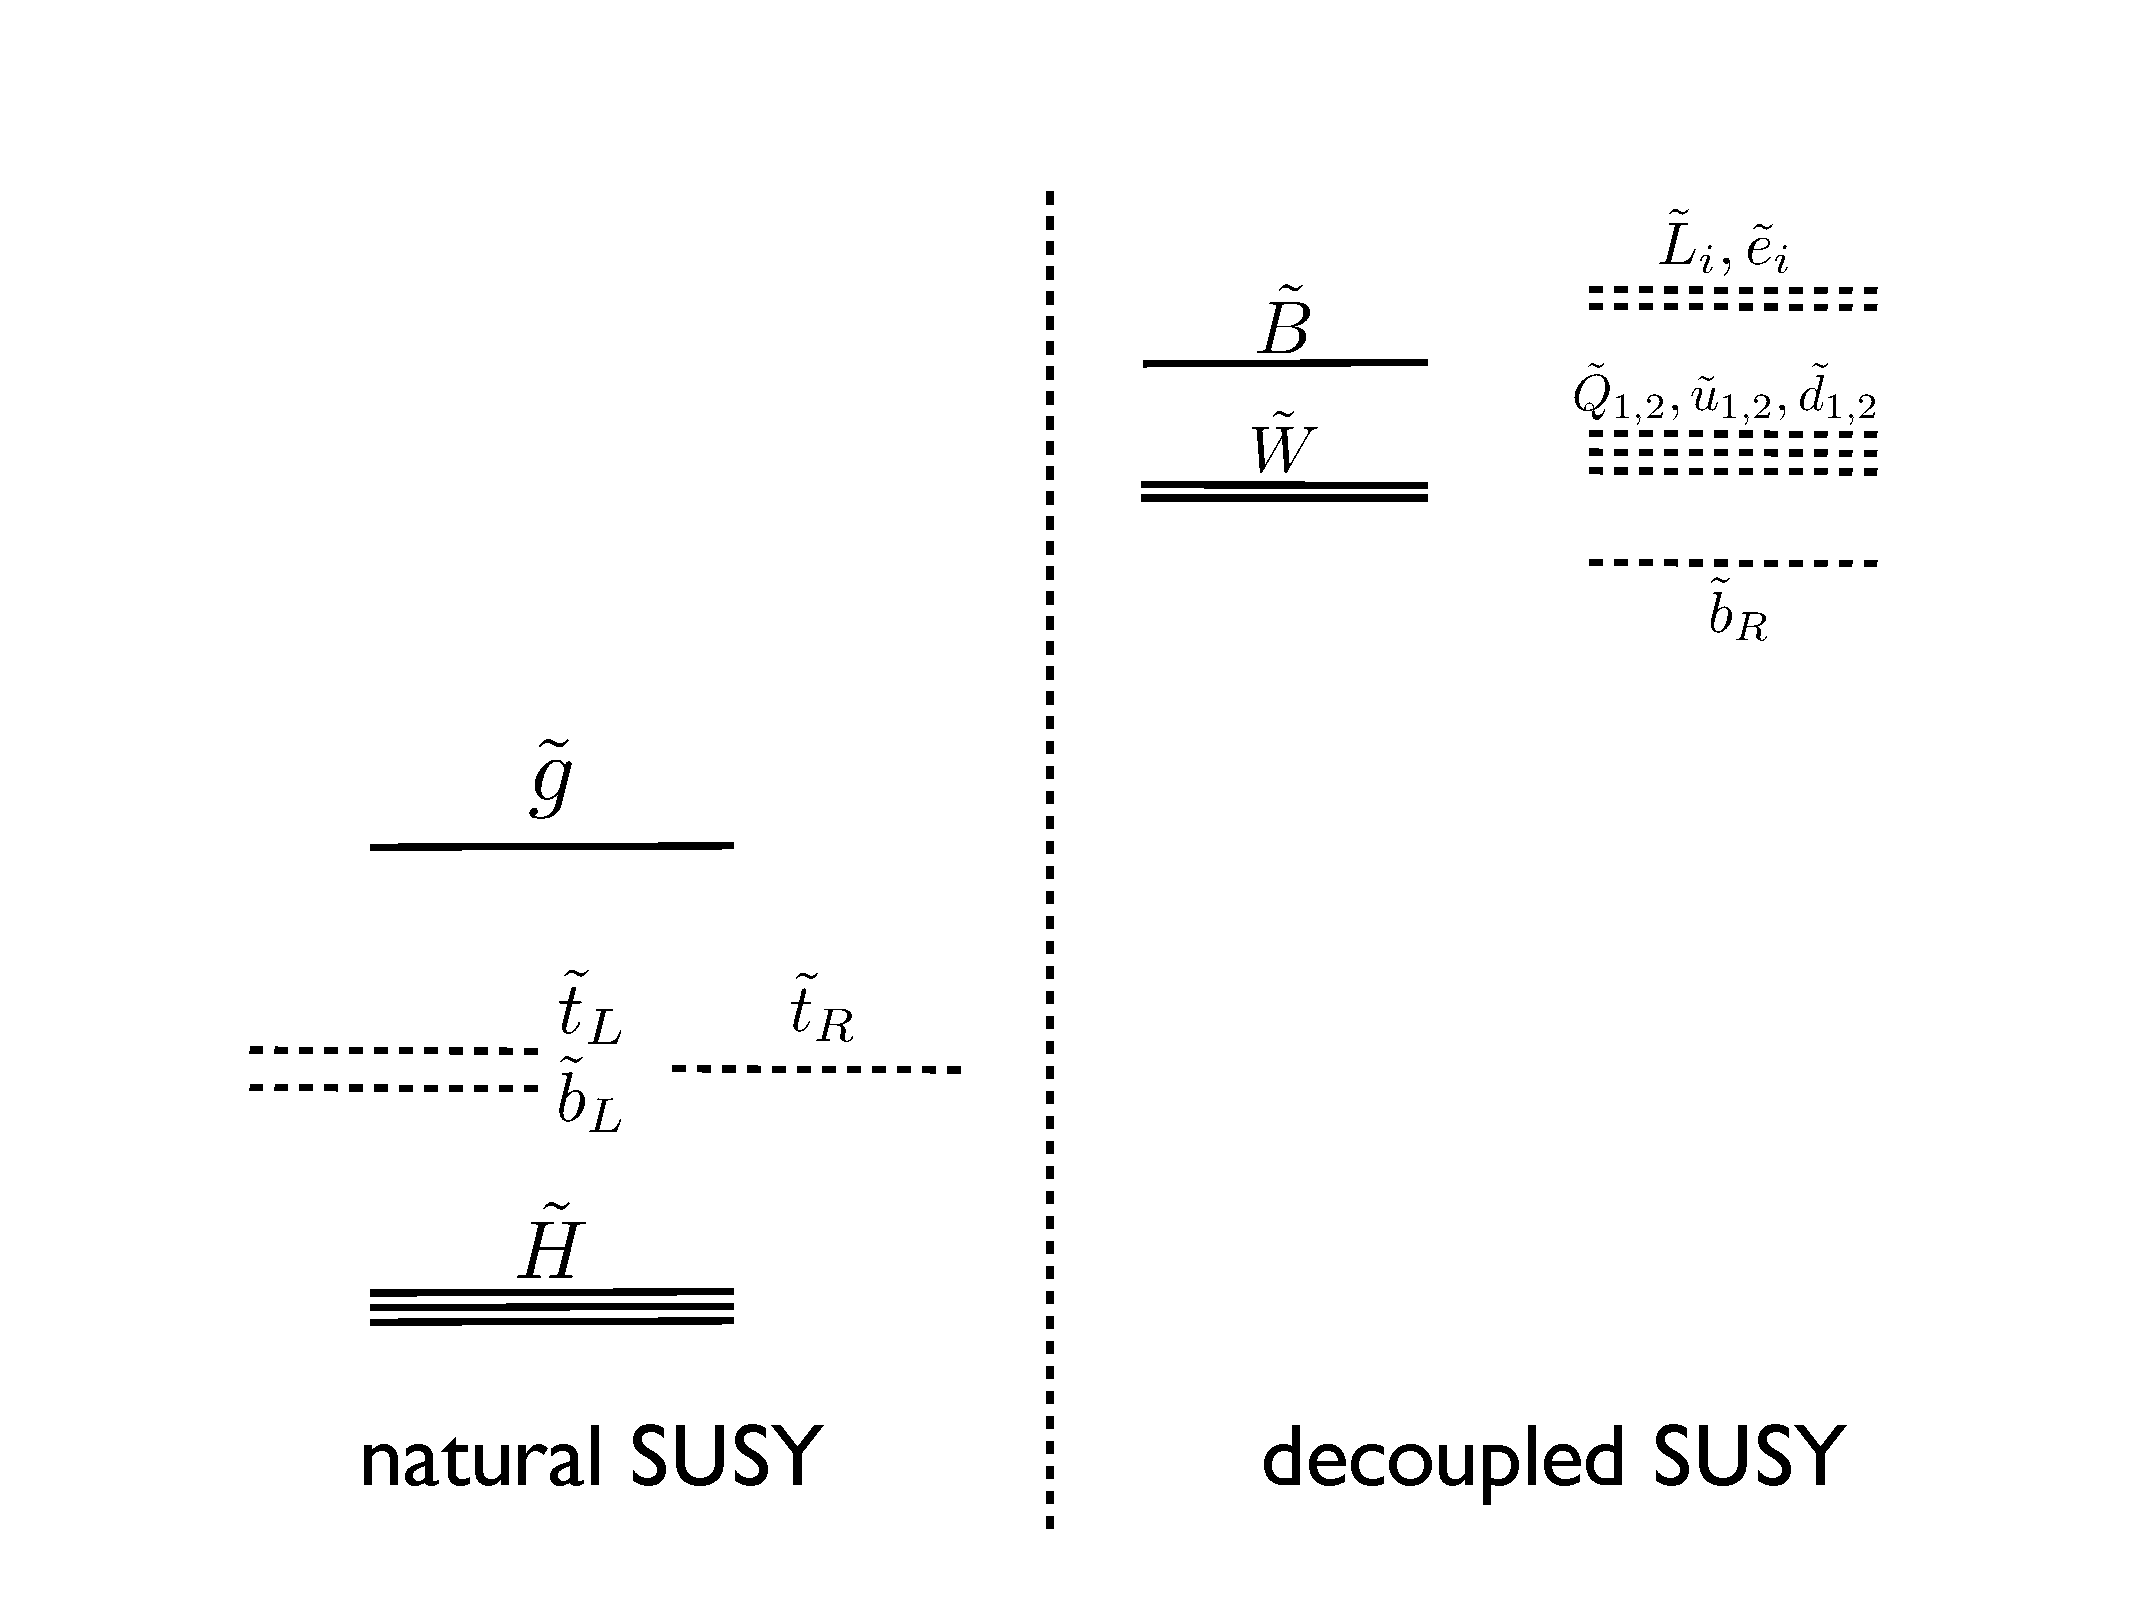
\includegraphics[width=0.9\textwidth]{figures/theory/NaturalSpec.pdf} 
\end{center}
\caption{The Naturalness argument constrains the masses of the \gls{susy} particles on the left side of the figure to be light, while the superpartners on the right side of the figure can have arbitrary mass without spoiling the Naturalness of the model. Figure from Ref. \cite{Papucci:2011wy}.}
\label{fig:NaturalSpectrum}
\end{figure}


\subsection{SUSY breaking in the MSSM}

Superpartners of the \gls{sm} particles have not been observed yet. This means that, if they exist, their mass must be larger than that of the corresponding \gls{sm} particle, and thus \gls{susy} must be a broken symmetry. The Lagrangian can therefore be written as:

\begin{equation}
\lagr = \lagr_{\rm SUSY} + \lagr_{\rm soft} \; ,
\end{equation}

\noindent where $\lagr_{\rm SUSY}$ is the \gls{susy}-conserving part derived from the superpotential, while $\lagr_{\rm soft}$ encloses the terms that break \gls{susy}. The suffix "soft" means that we allow in the Lagrangian only soft \gls{susy}-breaking terms, whose couplings have positive mass dimension, so that they vanish at very high mass scales. The inclusion of \gls{susy}-breaking terms requires the addition of new particles and interactions to the \gls{mssm}. While there is no unambiguous way to modify the theory to do this (some examples of \gls{susy}-breaking mechanisms are described in Section \ref{sec:susybreaking}), it is possible to include in the Lagrangian a general parametric form of the \gls{susy}-breaking terms:
\begin{itemize}
\item Gaugino masses, which in the \gls{mssm} correspond to the bino, wino and gluino mass terms;
\item Non-holomorphic scalar squared masses, which add mass terms for squarks and sleptons and contribute to the Higgs potential;
\item Holomorphic scalar squared masses, that in the \gls{mssm} can be present only in a term like $b H_u H_d$;
\item Scalar cubic couplings.
\end{itemize}  

The necessary \gls{susy}-breaking part of the Lagrangian adds to the \gls{mssm} many free parameters: in total the \gls{mssm} has 105 parameters in addition to the \gls{sm} ones.


\subsection{SUSY-breaking mechanisms}
\label{sec:susybreaking}

The \gls{susy}-breaking terms of $\lagr_{\rm soft}$ can be generated in models where \gls{susy} is spontaneously broken. This is the case if, just like  for the electroweak symmetry breaking, the Lagrangian is \gls{susy}-invariant, but the vacuum state is not. As it happens with the Higgs mechanism, the spontaneous breaking of a symmetry implies the appearance of a massless Goldstone particle (goldstino, $\stilde{G}$) that, in the case of \gls{susy}, has to be a neutral Weyl fermion in order to have the same quantum numbers as the supercharge $Q$. To be massless and annihilate the fermion mass matrix, the goldstino field has to be proportional to:

\begin{equation}
 \stilde{G} \,=\, 
 \begin{pmatrix}
\langle D^a \rangle /\sqrt{2} \cr \langle F_i\rangle 
\end{pmatrix} \; ,
\label{explicitgoldstino}
\end{equation} 

\noindent where $D^a$ and $F_i$ are respectively the auxiliary real bosonic and complex fermion fields of the \gls{susy} Lagrangian, and $\langle \rangle $ denotes their vacuum expectation value. For Equation \ref{explicitgoldstino} to be non-trivial, at least one of the $D^a$ or $F_i$ has to have a non-zero \gls{vev}. This is related to the two possible mechanisms that lead to \gls{susy} breaking: via a $D$-term or an $F$-term. 
The Fayet-Iliopoulos mechanism \cite{Fayet:1974jb} allows to have a non-zero \gls{vev} for an auxiliary field $D$ by adding to the Lagrangian a term proportional to the auxiliary field itself, and with a coupling constant with the dimension of a squared mass:
\begin{equation}
\lagr_{\rm FI} \,=\, -\kappa D \; .
\end{equation}
With this mechanism it is however difficult to attribute properly masses to all the \gls{mssm} particles.
%This type of term is gauge-invariant only for abelian groups. 
%the hypercharge symmetry group $U(1)_Y$ is not eligible 

Another possibility is to assign a \gls{vev} to an $F$-term, with the O’Raifeartaigh mechanism \cite{ORaifeartaigh:1975nky}. Since in the \gls{mssm} there is not a good candidate to be a gauge singlet with a non-vanishing \gls{vev} for an $F$-term, this implies the addition of at least one set of chiral supermultiplets, such that $F_i$ is non-trivial for at least one of them. A realization of this is possible for example with three chiral supermupliplets $\Phi_i$ and a superpotential of the form:
\begin{equation}
W = -k \Phi_1 + m \Phi_2 \Phi_3 + {y\over 2} \Phi_1 \Phi_3^2 \;.
\label{oraif}
\end{equation}
The resulting scalar potential at tree level has a minimum for $\phi_2=\phi_3=0$ and independent of $\phi_1$ (where $\phi_i$ are the scalar fields in $\Phi_i$), while the one-loop corrections highlight a non-zero global minimum when also $\phi_1=0$. In the following we will consider only \gls{susy} breaking originating from the O’Raifeartaigh mechanism.


When \gls{susy} is treated as a local symmetry, it has to include also gravity, and the resulting theory is called supergravity. The gravity mediator is the spin-2 graviton, and its superpartner the spin-$\frac{3}{2}$ gravitino. The gravitino can be interpreted as the gauge field of \gls{susy}, and it incorporates the goldstino degrees of freedom upon spontaneous \gls{susy} breaking. Therefore, the gravitino is also indicated with the same symbol as the goldstino, $\stilde{G}$. By dimensional arguments, we can understand that the gravitino mass ($m_{3/2}$) has to be proportional to:

\begin{equation}
m_{3/2} \approx \frac{\langle F \rangle}{\Lambda_P} \; ,
\label{mgrav}
\end{equation}
\noindent where $\langle F \rangle$ is the \gls{vev} of the \gls{susy}-breaking $F$-term, as it has to vanish both if \gls{susy} is an exact symmetry and if the Planck scale is extremely high (and thus gravity is negligible). 

For any \gls{susy}-breaking mechanism, the \gls{mssm} soft term do not appear at tree level, but are generated through radiative corrections. \gls{susy} breaking happens in a hidden sector, while the \gls{mssm} particle live in the visible sector, and experiment the consequences of the spontaneous \gls{susy} breaking happening in the hidden sector through interactions that couple both sectors. Depending on which interaction is driving the communication between the \gls{susy}-breaking sector and the \gls{mssm}, we can distinguish three main mechanisms:

\subsubsection*{PMSB} 

If supergravity and the other new physics effects that arise at the Planck scale are the responsible of the connection of the hidden sector with the \gls{mssm} sector, then the order of magnitude of the soft parameters in the \gls{mssm} is:
\begin{equation}
m_{\rm{soft}} \approx \frac{\langle F \rangle}{\Lambda_P} \; .
\label{msoft_PMSB}
\end{equation}
\noindent This ratio is motivated by the observation that $m_{soft}$ should vanish both in the limit where \gls{susy} is an exact symmetry, as well as in the limit where the Planck mass is very large and the interactions mediated by gravity are not anymore sizable. We refer to this scenario as \gls{pmsb} \cite{PhysRevLett.49.970, BARBIERI1982343, IBANEZ198273, PhysRevD.27.2359}. In \gls{pmsb} models, the gravitino mass has the same order of magnitude as the mass of the other superpartners (as we can notice by comparing Equation~\ref{mgrav} and Equation~\ref{msoft_PMSB}), and therefore it can not be particularly light. 

\subsubsection*{AMSB}

If the supregravity couplings that mediate \gls{susy} breaking in \gls{pmsb} models are absent, \gls{susy} can be broken through loop effects. In \gls{amsb} models \cite{Randall:1998uk,Giudice:1998xp} scalar and gaugino masses are generated through one-loop corrections arising from superconformal anomalies. These corrections are always present, but are dominant only in models that do not include tree-level terms. In the simplest \gls{amsb} model leads to the prediction of negative squared masses for sfermions; one possible extension to the model that solves this problem is the addition of a scalar mass parameter $m_0^2$, common to all scalar squared masses. 

\subsubsection*{GMSB}

In the case of \gls{gmsb} \cite{Dine:1981gu, AlvarezGaume:1981wy, Nappi:1982hm, PhysRevD.48.1277, Dine:1994vc, Dine:1995ag} the interactions mediating the connection between the hidden sector and the \gls{mssm} are the same gauge interactions of the \gls{mssm} itself. This requires to add to the theory a set of chiral supermultiplets (mediators) that interact both with the source of supersymmetry breaking and with the \gls{mssm} particles (through loop corrections to their masses, involving the \gls{mssm} gauge interactions). The mediators contribute at one loop to the mass of gauginos, while they have a two-loop contribution to the mass of squarks and leptons. In both cases, the mass scale of the superpartners is:
\begin{equation}
m_{\rm{soft}} \approx \frac{\langle F \rangle}{M_\mathrm{mediator}} \; .
\label{msoft_GMSB}
\end{equation}
\gls{sm} gauge bosons are not affected by the loop corrections induced by the mediators as their mass is protected by the gauge symmetry.
If we compare Equation \ref{msoft_GMSB} with Equation \ref{mgrav} we can see that, as long as the mass of the mediators is lower than the Planck scale, the gravitino can be significantly lighter than the rest of the superpartners. In most \gls{gmsb} models the gravitino is the \gls{lsp}, and all particles decay to it. While we could expect the decay rate to a $\stilde{G}$ to be low because of the weakness of the gravitational interaction, this is not the case as the gravitino inherits the gauge interactions of the goldstino it absorbs during the spontaneous supersymmetry breaking.  
\gls{susy} breaking introduces a large number of free parameters with respect to the \gls{sm}.
Most of these new parameters lead to flavor-changing interactions that are highly suppressed experimentally. 
In models of gauge mediation, the interaction between the \gls{susy}-breaking sector and the \gls{mssm} happens only through gauge interaction, that are flavor-blind, and therefore the suppression of flavor-changing effects is implemented automatically.



\subsection{Phenomenological MSSM}
\label{sec:theory:pmssm}

The \gls{pmssm} \cite{Djouadi:1998di} reduces the number of free parameters in the \gls{mssm} through some assumptions motivated by experimental evidence. In particular:
\begin{itemize}
\item To avoid flavor changing neutral currents, the sfermion mass matrices and all the trilinear couplings are diagonal. 
\item The presence of CP-violating terms is bound to be only the one predicted by the \gls{sm} by imposing that all the new parameters are real numbers.
\item The first two generations of sfermions are degenerate i.e. the corresponding elements in the first and second generation have the same mass, to circumvent existing limits on the splitting between the first ans second squark generations.
\item Since the trilinear couplings give rise to amplitudes that are proportional to the corresponding Yukawa coupling, only the third generation ones are relevant and the others are set to zero.
\end{itemize}

These assumptions allow to reduce the number of free parameters from 105 to 19 (summarized in Table \ref{tab:pMMSpar}), making phenomenological analyses possible.


\begin{table}[h]
\centering
\begin{tabular}{c c}
\hline 
Parameter & Description \\ 
\hline 
\hline
$M_1, M_2  \, M_3 $ & Gaugino mass parameters \\ 
\hline 
$\tan \beta$ & Ratio of the \glspl{vev} of the two Higgs doublets \\ 
\hline 
$M_A$ & Pseudoscalar Higgs boson mass parameter \\ 
\hline 
$\mu$ & higgsino mass parameter \\ 
\hline 
$  A_t, \, A_b, \, A_\tau    $ & Third generation trlinear couplings \\ 
\hline 
$m_{qL},  \,  m_{uR},  \, m_{dR},  m_{lL},  \, m_{eR}$ & First (and second) generation sfermion masses \\ 
\hline 
 $m_{q3L}, \, m_{tR}, \, m_{bR}, \, m_{\stilde{L}}, \, m_{\stilde{\tau}_R},$ & Third generation sfermion masses \\ 
\hline 
\end{tabular} 
\caption[Free parameters of the \gls{pmssm}]{\label{tab:pMMSpar}List of free parameters in the \gls{pmssm}.}
\end{table}





% Supersymmetry (SUSY) is a \gls{bsm} framework that allows to generate an infinite amount of \gls{bsm} models, each with different signatures.

\chapter{LHC and \gls{atlas}}
\label{chap:cern}

The analyses presented in this thesis use the \gls{pp} collision data at a center-of-mass energy \cmtre TeV 
collected by the \gls{atlas} experiment in 2015, 2016 and 2017. 

The \gls{atlas} experiment is one of the four main experiments at the \gls{lhc} at the \gls{cern}. Section \ref{sed:cern:lhc} of this chapter describes the \gls{lhc} accelerator complex. This is followed by a general description of the detectors used in high-energy physics in Section \ref{sec:detectors}. The \gls{atlas} detector is discussed in Section \ref{sed:cern:atlas}.

%%%%%%%%%%%%%%%%%% LHC

\section{The Large Hadron Collider}
\label{sed:cern:lhc}

In this section we give a brief introduction to the \gls{lhc} \cite{1748-0221-3-08-S08001}, at the moment the largest and most powerful particle accelerator in the world, hosted by \gls{cern} and in operation since September 2008.


\subsection{A circular hadron collider}

The \gls{lhc} is a circular hadron accelerator, located in a 26.7-km-long underground tunnel (with a depth ranging between 50 and 140 meters) that was previously hosting the \gls{lep}, a \gls{cern} accelerator that was operational from 1989 to 2000. The \gls{lhc} can accelerate protons up to a design center-of-mass energy of 13 TeV. Accelerating particles to very high energies is necessary both to study the structure of the particles themselves at smaller scales, and to create heavy states in collisions. Cosmic rays provide a source of particles with energies up to $10^7$ times more than what the \gls{lhc} is capable of, but these extremely energetic rays are very rare, and the flux is not controlled. Accelerators provide a well controlled flux of particles of a specific type in a specific location, and this allows the study of these particles with dedicated detectors.

A circular accelerator simplifies the acceleration of particles, as this can happen over several revolutions. When a charged particle travels on an orbit of radius $r$ under the effect of a magnetic field $B$, its momentum $p$ is given by:
\begin{equation}
\label{eq:cern:p03br}
p = 0.3 r B,
\end{equation}
\noindent where the momentum is expressed in GeV, B in Tesla and the radius of the orbit in meters. For a given magnetic field, a larger radius allows to reach higher energies. 

The choice of a collider over a fixed-target experiment is motivated by the possibility of reaching a higher energy in center-of-mass of the system: while in a fixed-target experiment this is proportional to the square root of the energy of the incoming particle, in a collider it is the sum of the energies of the two beams.


Suitable particles for a collider experiment need to fulfill two criteria: they need to be charged, in order to be accelerated and guided through electric and magnetic fields, and they need to be stable enough not to decay before being used for collisions. These criteria effectively limit the choice to protons, electrons, their antiparticles and ions. 

At the \gls{lhc} it has been chosen to study collisions with protons and lead ions. Three types of collisions are studied: proton-proton ($p-p$), lead-lead ($Pb-Pb$) and also proton-lead ($Pb-p$). The main reason to prefer protons over electrons is the energy loss that affects charged particles accelerated in a circular trajectory (\textit{syncrotron radiation}), which decreases with the fourth power of the mass of the particle:

\begin{equation}
\label{eq:cern:sync}
\frac{dE}{dt} \propto \frac{E^4}{m^4 r^2} \; .
\end{equation}

The larger mass of a proton with respect to an electron leads to a decrease by a factor $10^{12}$ in the energy lost through syncrotron radiation. This choice comes with a price: proton-proton collisions lead to less clean events, with a lot of soft interactions covering the interesting hard interactions. Furthermore, the center-of-mass energy is unknown as the particles taking part in hard interactions are not the protons themselves but their constituents.

\subsection{Magnet system} 


The \gls{lhc} is not a perfect circumference: it is composed of eight arcs (\textit{sectors}), where the magnetic system is located, and eight straight sections containing the resonant cavities, the four interaction points with and the detectors, the equipment for beam injection and extraction, and other instrumentation. Magnetic fields are used to govern the trajectory of particles. In the \gls{lhc} there are more than nine thousand magnets, constructed from a superconducting alloy of niobium and titanium. About 150 tons of super-fluid helium at a temperature of 1.9 K are used to maintain the magnet system in the superconducting regime. Different types of magnets are necessary to achieve a proper control over the trajectory of particles.

\subsubsection*{Dipoles} 
Dipoles are used to create a vertical magnetic field, so as to bend the particles in the horizontal plane and thus give the dominant circular orbit. The \gls{lhc} has 1232 dipoles, each 15 m long and providing a magnetic field of 8.3 T. The current necessary to achieve this strong magnetic field is 11.8 kA.


\subsubsection*{Quadrupoles}
The \gls{lhc} has 858 quadrupoles, used for beam focusing. A single quadrupole can focus the beam either in the vertical or the horizontal plane, but it causes a defocusing in the other plane; conventionally a quadrupole is denoted as focusing if it is oriented to focus in the horizontal plane. A combination of focusing and defocusing quadrupoles separated by some drift space (\textit{FODO lattice}) is used to keep both planes focused, and gives rise to \textit{Betatron oscillations}. Figure \ref{fig:lhc:quad} shows a schematic representation of the transverse view of a quadrupole magnet.

\subsubsection*{Higher-order magnets} 
Beside dipoles and quadrupoles, in the \gls{lhc} there are about 600 higher-order magnets that are used to maintain a good beam quality; e.g.  sextupoles are used to correct the spread in Betatron tune caused by the quadrupoles.




\begin{figure}[ht]
\centering
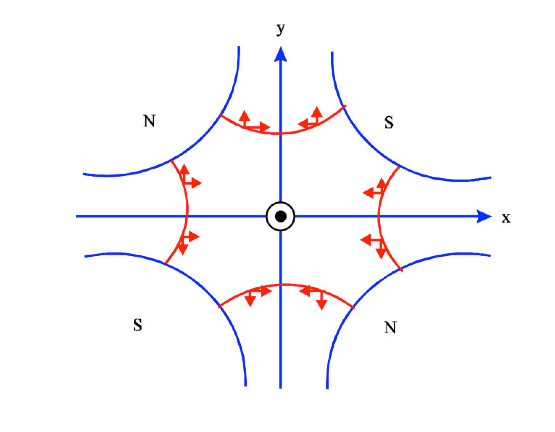
\includegraphics[width=0.45\textwidth]{figures/lhc/figures_quad}
\caption{A schematic cross-section of a quadrupole magnet. The red arrows indicate the direction of the force experienced by the particle. Figure from Ref. \cite{Kain:2016aly}.}
\label{fig:lhc:quad}
\end{figure}

\subsection{Resonant cavities}

While the orbit of particles is governed by the magnetic fields, longitudinal electric fields are used for acceleration. In the \gls{lhc} the electric filed is provided by \gls{rf} cavities. There are overall 16 \gls{rf} cavities, eight per beam, hosted in four cryo-modules. Each cavity can provide an accelerating field of 5 MV/m, and oscillates with a frequency of 400 MHz. Since the electric field changes over time with the oscillations, particles passing through the same point of a \gls{rf} cavity at different times experience a different voltage; this produces a non-trivial longitudinal dynamics, where particles oscillate around the ideal synchronous particle with changes in momentum and phase (\textit{Synchrotron oscillations}). If we define the \textit{slip factor} $\eta$ as the relative change in frequency in Synchrotron oscillations with the relative change in momentum:
\begin{equation}
\eta = \frac{\Delta f / f}{\Delta p / p} \; ,
\end{equation}

\noindent and the compaction factor $\alpha$ as the relative change in frequency in orbit length with the relative change in momentum:

\begin{equation}
\alpha = \frac{\Delta L / L}{\Delta p / p} \; ,
\end{equation}

\noindent the following relation holds:

\begin{equation}
\eta = \frac{1}{\gamma^2} - \alpha \; ,
\end{equation}

where $\gamma$ is the Lorentz factor of the particle. This means that while the energy of the particle is low ($\eta>0$) an increase in momentum leads to an increase in frequency, while it leads to a decrease in frequency for $\eta<0$. At the transition energy, a previously stable synchrotron phase becomes unstable and vice versa; this requires a rapid change in \gls{rf} phase. This situation is illustrated in Figure \ref{fig:lhc:phase}(a). For example, a particle corresponding to the phase point M1 will arrive in the \gls{rf} cavity after one corresponding to the stability point P1, and will experiment higher voltage and increase in momentum; if $\eta>0$ this increase in momentum will translate in an increase in frequency and the particle will, at the following revolution, arrive earlier, while if $\eta<0$ the frequency will further decrease and the particle will be eventually lost.  The transition energy in the \gls{lhc} is 53 GeV, well below the injection energy of 450 GeV, so the \gls{lhc} is always above transition. 

\begin{figure}[ht]
\centering
\subfigure{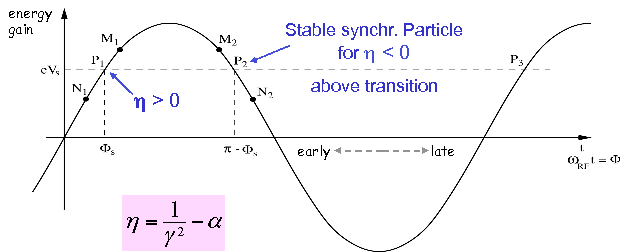
\includegraphics[width=0.547\textwidth]{figures/lhc/phase-stability-2}}
\subfigure{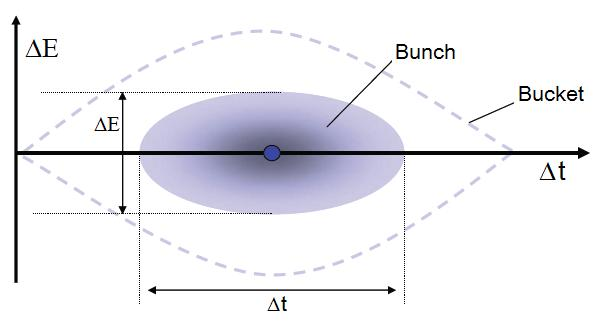
\includegraphics[width=0.44\textwidth]{figures/lhc/bucket}}
\caption{(a) Phase stability below and above transition. Figure from Ref. \cite{Tecker:2016mlq}. (b) Bucket and the bunch for a beam above the transition energy. Figure from Ref. \cite{Baird:1017689}.}
\label{fig:lhc:phase}
\end{figure}


In the \gls{lhc} beams particles are not distributed continuously, as this would now be allowed by phase instabilities, but are divided in \textit{bunches}. 
The areas of stable motion are identified as \textit{bucket}, and the area of the bucket is the beam \textit{longitudinal acceptance}. The beam bunches fill only a part of the bucket, and the area of the beam bunches is the \textit{longitudinal beam emittance}. Figure \ref{fig:lhc:phase}(b) shows a schematic view of the bucket and the bunch area for the case of a beam above the transition energy. 

\subsection{Luminosity and operational parameters}

The amount of data delivered by an accelerator is quantified by the \textit{integrated luminosity} $\mathcal{L}_{int}$.
Given a certain process with production cross section $\sigma$, the total number of events for that process is the product of cross section and integrated luminosity:

\begin{equation}
\label{eq:cern:nev}
N_{\mathrm{events}} = \sigma \,\, \mathcal{L}_{int} \; .
\end{equation}

The integrated luminosity is the time integral of the \textit{instantaneous luminosity} $\mathcal{L}$, 

\begin{equation}
\label{eq:cern:intlumi}
\mathcal{L}_{int} = \int \mathcal{L} \, dt \; ,
\end{equation}

\noindent which, assuming a Gaussian particle distribution and the same characteristics for the two beams, can be expressed as:

\begin{equation}
\mathcal{L}=\frac{f N_b n^2}{4 \pi \sigma_{x}\sigma_{y} } \; ,
\label{eq:cern:lumi}
\end{equation}

\noindent where $f$ is the revolution frequency, $N_b$ the number of bunches in each beam, $n$ the number of protons in each bunch and $\sigma_{x(y)}$  is the transverse beam size at the interaction point in the $x$($y$) direction . 

The instantaneous luminosity defined in Eq. \ref{eq:cern:lumi} needs to be corrected for two effects. First of all, this formula assumes a head-on collision between the bunches; in reality, to avoid unwanted interactions the beams collide with a crossing angle, and a large crossing angle decreases the instantaneous luminosity. The second correction is related to the beam transverse size, that can be expressed as:
\begin{equation}
\sigma_{x,y} = \sqrt{  \epsilon \beta^* } \; ,
\end{equation}
where $\epsilon$ is the beam emittance and $\beta^*$ is the \textit{beta function}. Beam collisions happen in \textit{minibeta insertions}, drift spaces with a beta waist in the center, where the beam size is as small as possible. In the vicinity of the minimum, the beta function evolves like:

\begin{equation}
\beta(s) = \beta^* + \frac{s^2}{\beta^*} \; .
\end{equation}

From this it is possible to see that the smaller the beta function, the larger the dependence with $s$, so a bunch with a finite size will not have the same beta function as a whole (\textit{hour glass effect}). This correction becomes more important with the decrease of the $\beta^*$ value. With the \gls{lhc} design parameters, the effect of crossing angle and hour glass changes the instantaneous luminosity by about 20\%.

The main limitations in the choice of the parameters that regulate the luminosity are \textit{collective effects}, which could cause beam instabilities if the number of bunches or the number of protons per bunch is too high, and the limitations in the available aperture in the
quadrupoles focusing the beam in the minibeta insertions, that impacts $\beta^*$. The summary of the \gls{lhc} operational parameters during Run 2 is reported in Table \ref{tab:lhc:param}.


\begin{table}[ht]
\begin{center}
\begin{tabular}{c c c c c }
\hline 
Parameter & 2015 & 2016 & 2017 & Design \\ 
\hline 
\hline
Protons per bunch (n) [$10^{11}$ p] & $\approx$ 1.2 & $\approx$ 1.1 & $\approx$ 1.2 & 1.15 \\ 
\hline 
Number of bunches (N$_b$) & 2244 & 2220 & $\approx$ 2250 & 2780 \\ 
\hline 
Emittance ($\epsilon$) [mm mrad] & $\approx$ 3.5 & $\approx$ 2.2 & $\approx$ 2.2 & 3.5 \\ 
\hline 
Beta function ($\beta^*$) [cm] & 80 & 40 & 40 (30) & 55 \\
\hline
Crossing angle [$\mu$rad] & 290 & 370 (280) & 300 (340) & 285 \\
\hline
Peak luminosity [$10^{34}$ cm$^{-2}$s$^{-1}$] & 0.51 & 1.4 & 1.7(1.9) & 1.0 \\
\hline
\end{tabular}
\end{center}
\caption{\gls{lhc} operational parameters in Run 2 compared to their design value.
The numbers in parenthesis report changes in the parameters during the year. 
E.g. in 2016 the crossing angle was reduced after fill 5300,
while for 2017 the numbers in parenthesis report the values 
after the recommissioning with $\beta^* = 0.3$ m.}
\label{tab:lhc:param}
\end{table}


The luminosity profile changes over time, and different experiments have different luminosity needs. \gls{atlas} and CMS profit from having the maximum luminosity possible, while LHCb and ALICE have their top functionality at lower luminosity, and therefore apply a \textit{luminosity leveling} that consists in changing the offset of the beams during the run, to maintain a constant (low) value of the instantaneous luminosity.

A high number of particles participating in a single bunch crossing can lead to a large number of multiple proton-proton collisions (\textit{pileup}). In 2012 the \gls{lhc} operated with a bunch spacing of 50 ns, leading to a pileup of about 35 events per bunch crossing. With the increase in energy from Run 1 to Run 2, the same settings would have implied more than 100 events, above the limit for the proper functioning of the detectors. This is what motivated the choice to move from the 50 ns bunch spacing used in Run 1 to the 25 ns in Run 2: with this setup, for the same instantaneous luminosity is possible to have a lower "luminosity per bunch" and therefore a lower pile up. Figure \ref{fig:atlas:pu} shows the luminosity-weighted distribution of the mean number of interactions per crossing during Run 1 (in Figure \ref{fig:atlas:pu:run1})
and in 2015-2017 (in Figure \ref{fig:atlas:pu:run2}) as recorded by the \gls{atlas} experiment.

\begin{figure}[ht]
\centering
\subfigure{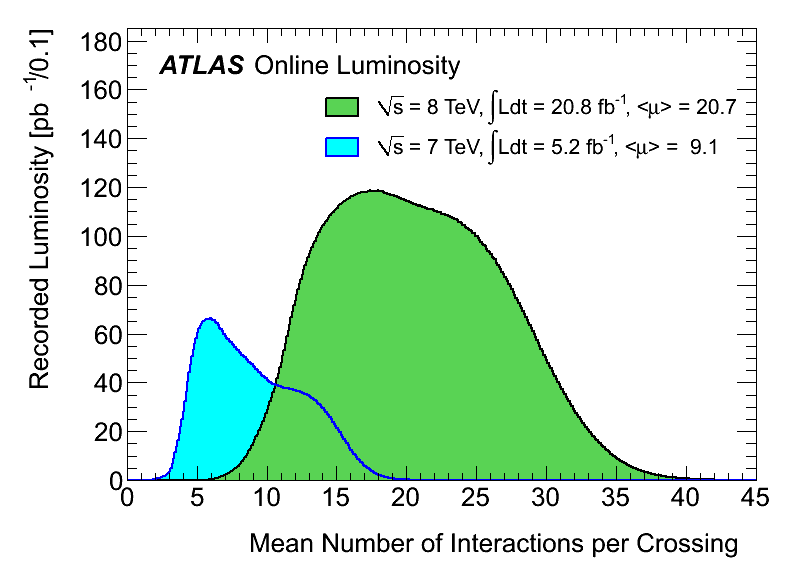
\includegraphics[width=0.49\textwidth]{figures/atlas/lumi/pu_profile_run1}\label{fig:atlas:pu:run1}}
\subfigure{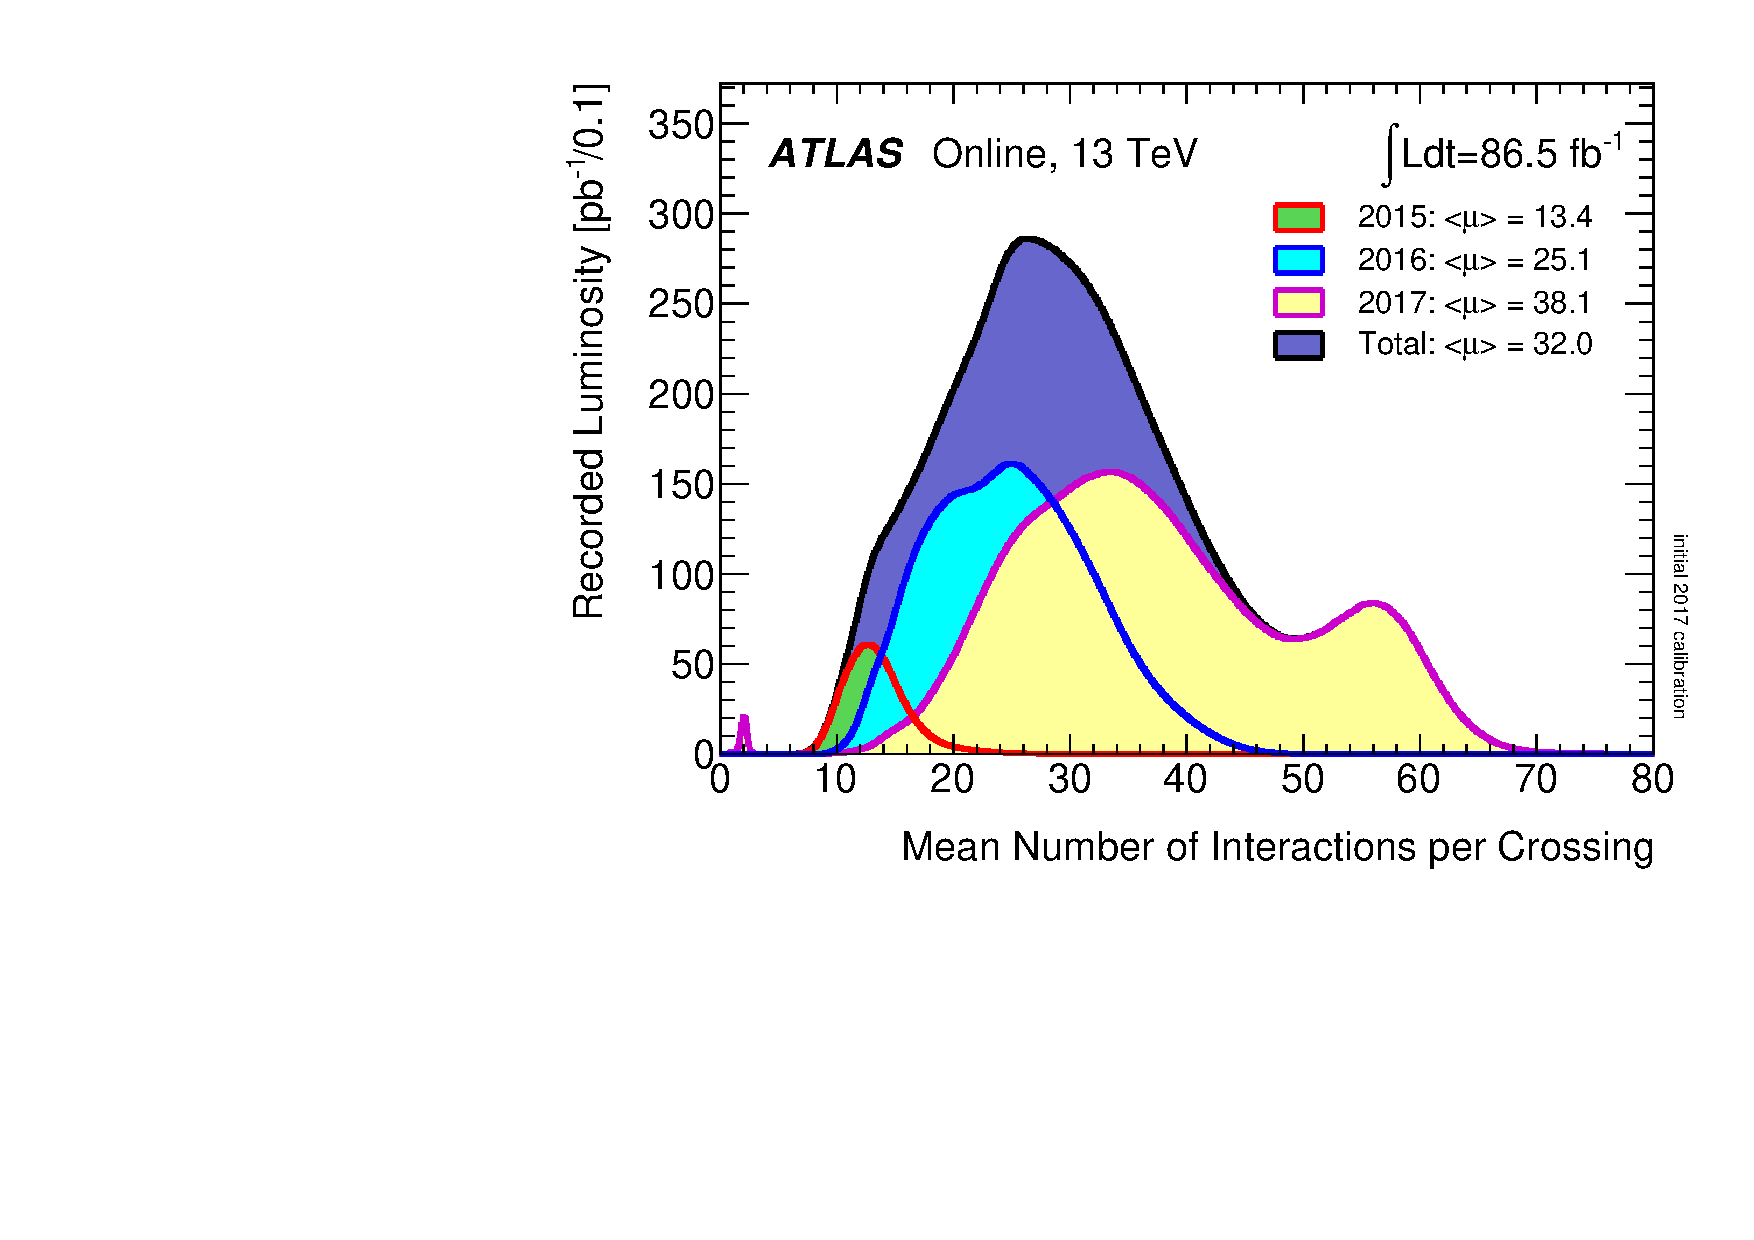
\includegraphics[width=0.49\textwidth]{figures/atlas/lumi/pu_profile}\label{fig:atlas:pu:run2}}
\caption{Luminosity-weighted distribution of the mean number of interactions per crossing in 
\subref{fig:atlas:pu:run1} Run 1 and \subref{fig:atlas:pu:run2} Run 2 (2015-2017). All data recorded by \gls{atlas} during stable beams is shown. The mean number of interactions per crossing $\mu$ corresponds to the mean of the Poisson distribution of the number of interactions per crossing calculated for each bunch. It is calculated from the instantaneous per-bunch luminosity as 
$\mu = \frac{\mathcal{L}_{bunch}\times \sigma_{inel}}{f}$, where $\mathcal{L}_{bunch}$ is the per-bunch instantaneous luminosity, $\sigma_{inel}$ is the inelastic cross section which is taken to be 80 mb for 13 TeV collisions, and $f$ is the \gls{lhc} revolution frequency. Figures from Ref. \cite{LumiTwiki}.}
\label{fig:atlas:pu}
\end{figure}


\subsection{Accelerator complex}

Protons are injected in the \gls{lhc} only after being accelerated to 450 GeV by a sequence of machines.

\begin{itemize}
\item Protons are extracted from a $H_2$ at the \textit{Linac2} facility, a linear accelerator of 33 m that brings them to the energy of 50 MeV.
\item The \gls{psb} is the first synchrotron in the acceleration chain (with a circumference of 157 m), that in 1.2 s increases the energy of the protons from 50 MeV to 1.4 GeV.
\item With a circumference of 628 m, the \gls{ps} brings the protons to about 26 GeV. This was the oldest synchrotron experiment at \gls{cern}.
\item The \gls{sps} is the first accelerator of the chain to be underground (about 30 m) and has a circumference of 6.9 km; it brings the proton energy at 450 GeV. Beside preparing the protons to be injected into the \gls{lhc}, the \gls{sps} provides beam also to the North Area, and to the AWAKE experiment, that studies proton-induced plasma wakefield acceleration.
\item The \gls{lhc} is the last step of this chain, and it accelerates the protons form 450 GeV to 6.5 TeV (the design energy is 7 TeV); while in the \gls{lhc} the protons gain about 0.5 MeV per turn, so it takes about 15 minutes to reach 6.5 TeV.
\end{itemize}

The accelerator complex of \gls{cern} is shown in Figure \ref{fig:lhc:acc}. The acceleration chain for lead ions is the same, except that the extraction and first acceleration is performed by \textit{Linac3} instead than by Linac2.

\begin{figure}[ht]
\centering
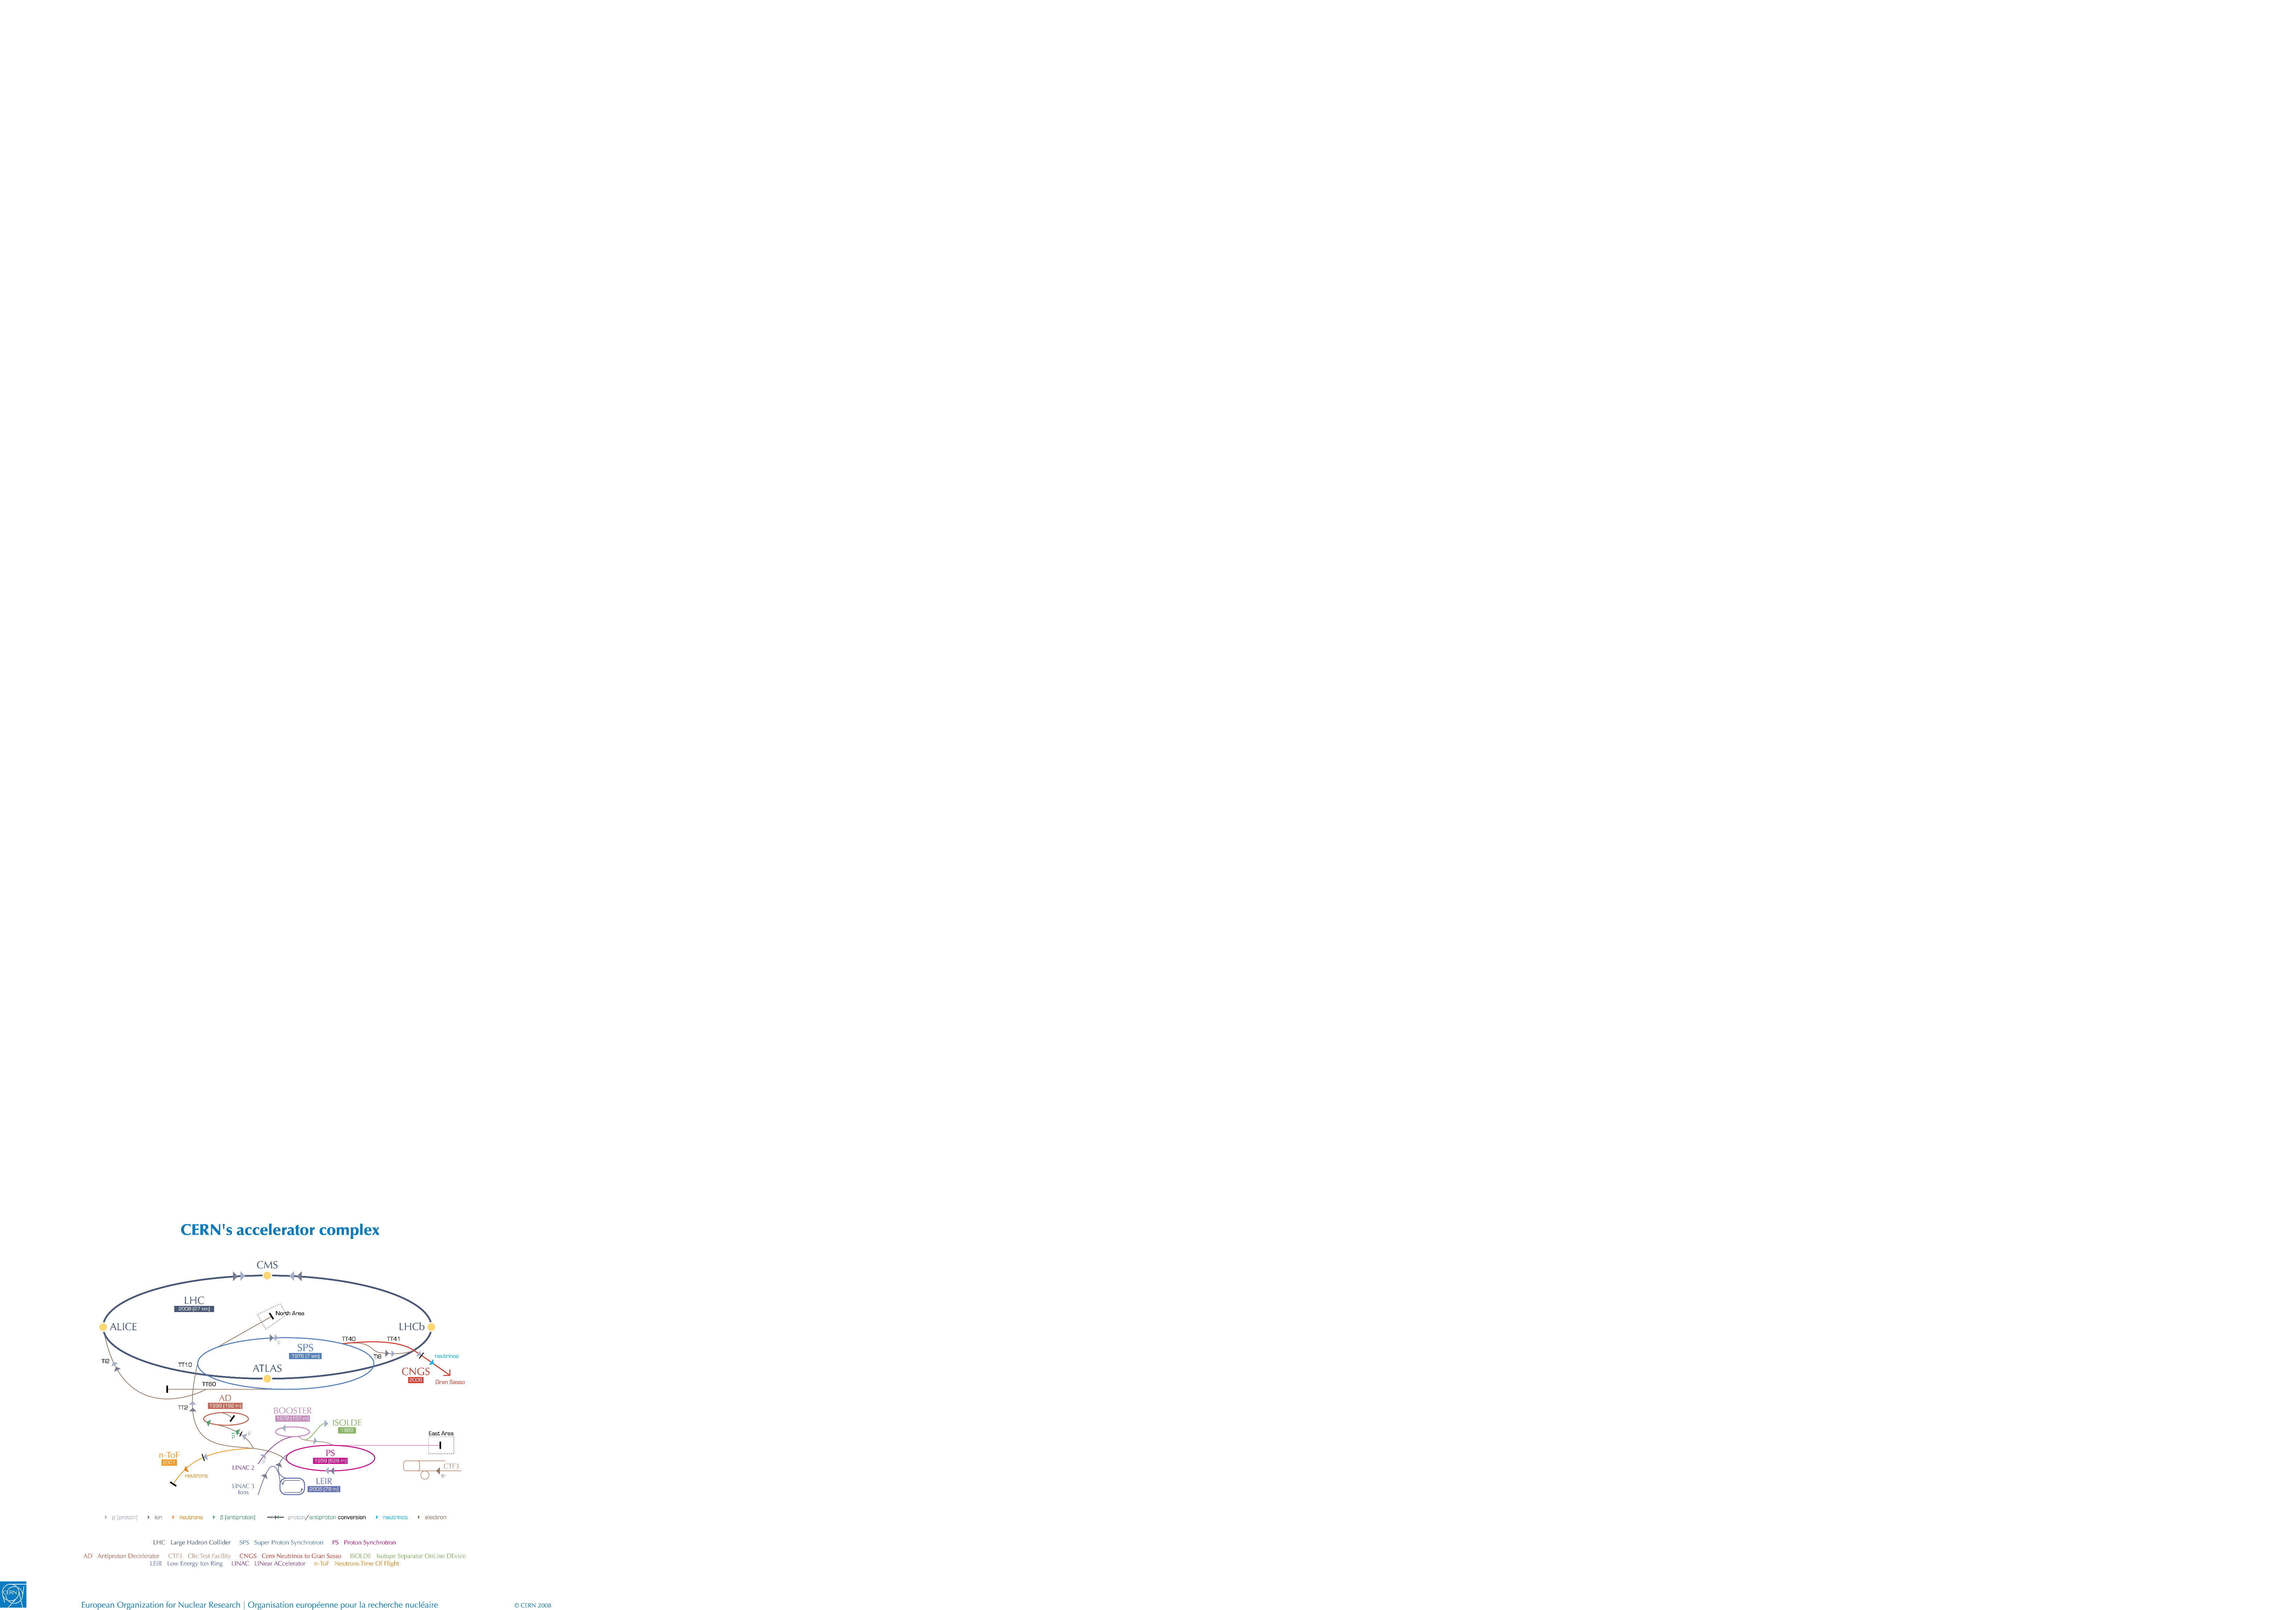
\includegraphics[width=1\textwidth]{figures/lhc/acc_complex.pdf}
\caption{ Schematic view of the \gls{cern} accelerator complex. The four main \gls{lhc} experiments are shown at the interaction points. Figure from Ref. \cite{Christiane:1260465}.}
\label{fig:lhc:acc}
\end{figure}

\subsection{Experiments at the LHC}

Seven experiments are built along the \gls{lhc} circumference and collect the data produced during the collisions. Each experiment is run by an independent collaboration that comprises several universities and research institutes. 
\textit{\gls{atlas}} \cite{atlas:atlas} and \textit{CMS} \cite{cms:cms} are the two largest and general purpose experiments, located at two opposite sides of the \gls{lhc} ring, in correspondence with two of the four interaction points. Their goal is to study a large variety of SM processes and to perform an extensive search program for \gls{bsm} physics. The independent design of the two detectors, as well as of the separation between the two collaborations running them, is essential to provide a validation of the \gls{lhc} results. Since the data used in this thesis is collected with the \gls{atlas} detector, a more extensive description of this experiment is given in Section \ref{sed:cern:atlas}. 
The \textit{LHCb} \cite{lhcb:lhcb} and \textit{ALICE} \cite{alice:alice} experiments are located at the other two \gls{lhc} interaction points. LHCb is a single-arm forward spectrometer, designed to perform high-precision studies of heavy flavour physics. The ALICE experiment is dedicated to the study of $Pb-Pb$ collisions, which at the \gls{lhc} happen with a center-of-mass energy of 2.6 TeV per nucleon pair; in this energy regime, quarks and gluons are expected to form a quark-gluon plasma.
The position of the four main experiments on the \gls{lhc} ring is shown in Figure \ref{fig:lhc:acc}.
Other three smaller experiments are installed along the \gls{lhc} circumference: TOTEM \cite{totem:totem}, LHCf \cite{lhcf:lhcf} and MoEDAL \cite{moedal:moedal}. TOTEM is located at the same interaction point as CMS, and measures the total $p-p$ cross section, as well as elastic and inelastic scattering. LHCf is installed in the same interaction point as \gls{atlas} and has two detectors, at 140 m from each side of the collision point, aiming at the study of particles produced in the "forward" region (very close to the beam axis). MoEDAL is installed in the LHCb cavern and is designed to search for magnetic monopoles.  


%%%%%%%%%%%%%%%%%% 

\section{Detectors for High Energy Physics}
\label{sec:detectors}

In this section we review the basic concepts that drive the design of the LHC detectors, including ATLAS.

\subsection{Identification of Particles}

The ability to accurately identify particles and reconstruct their energy is what drives the design of detectors for high energy physics. In a detector, different sub-systems are able to capture different types of particle interaction, and the combination of the information collected by each of them allows to identify particles (or at least assign them to families, such as neutral or charged hadrons). A typical schema of the subdetectors sequence is shown in Fig. \ref{fig:detector:interaction}. The innermost layer, closer to the interaction point, is the \textit{tracking system}, dedicated to the measurement of the signed change and momentum of charged particles. The following layers are the electromagnetic and hadronic \textit{calorimeters}, that measure the energy of particles with electromagnetic and hadronic interactions respectively. The outermost layer is dedicated to the \textit{muon system}: because of their large mass (about 200 times more than electrons) muons do not produce electromagnetic showers and are therefore easy to identify as they are the only particles that reach the external part of the detector.

\begin{figure}[ht]
\centering
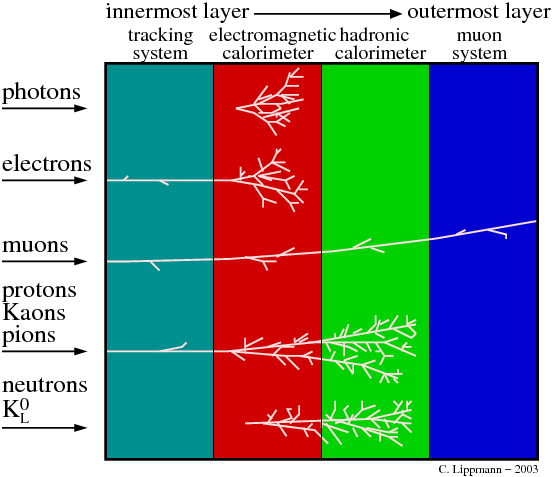
\includegraphics[width=0.6\textwidth]{figures/detector/particles_in_detector}
\caption{Components of a typical detector for physics at colliders. Different particles are identified by the distinctive signatures in the subdetectors. Figure from Ref. \cite{Lippmann:2011bb}.}
\label{fig:detector:interaction}
\end{figure}


\subsection{Tracking and Spectrometry}
\label{sec:dec:tracking}
A tracking device measures the traces left by charged particles passing through it. To allow the determination of the momentum and the charge of a particle, a tracking device needs to be accompanied by a magnetic field. 

The relative uncertainty on the momentum is given by:
\begin{equation}
\frac{\sigma_p}{p} = \frac{p}{0.3 B L^2}\sigma \sqrt{C_N}
\end{equation}


\subsection{Calorimetry}
\label{sec:dec:calo}

Calorimeters can measure the energy of both charged and neutral particles through a destructive measurement: the energy of the particles is deposited in the detector material and transformed into a measurable quantity. Because of their sensitivity to a wide variety of particles, good energy resolution and relatively small size, they are very attractive devices for accelerator physics experiments \cite{RevModPhys.75.1243} \cite{Wigmans:2000vf}.

When the incident particle interacts with the material of the calorimeter it develops a cascade of particles (\textit{shower}), with different characteristics for electromagnetic and hadronic interactions, described in the next two sections. Different types of calorimeters are necessary to capture the two typologies. The energy of the shower is decreased by the interactions happening in the \textit{absorber} material, while the \textit{active} material provides the conversion of the energy in a charge or light signal. In \textit{sampling calorimeters} layers of absorber and active material are alternated in sequence, while in \textit{homogeneous calorimeters} a single material carries out both functions.

We have noticed in section \ref{sec:dec:tracking} how the resolution of the momentum measurement in a magnetic spectrometer decreases with the increase of the momentum itself. Instead, the relative energy resolution in a calorimeter improves for high-energy particles, and can be written in the parametric form:

\begin{equation}
\frac{\sigma_E}{E} = \sqrt{\left(\frac{a}{\sqrt{E}} \right)^2 + \left( \frac{b}{E} \right)^2 + c^2 } \; .
\end{equation}

The first term of the sum in quadrature reflects the \textit{stochastic} nature of the shower development: ignoring the instrumental effects, the energy resolution of a calorimeter is proportional to the square root of the total track length, which is in turn proportional to the initial energy. The contribution of this term is small in homogeneous calorimeters, while is larger in sampling calorimeters (because of fluctuations of the fraction of energy deposited in the absorber) and it grows with the thickness of the absorber layers; typical values for $a$ are 5-20\% if the energy is expressed in GeV. The second term is the \textit{noise term} coming from the electronic noise of the readout chain; this term is in general more relevant for calorimeters producing charge signals than for those producing light signals, and can become the dominant term for particles with energy below one GeV. The last term is a constant deriving from instrumental effects that produce a non-uniform detector response, including for example energy lost outside the detector volume and radiation damage; this becomes the dominant term at high energies and is typically $<1\%$. 

\subsubsection{Electromagnetic Cascade}

When electrons, positrons and photons with energies above 1 GeV traverse a block of material the produce a cascade of particles (\textit{electromagnetic shower}): electrons and positrons can emit a photon by Bremsstrahlung, and a photon (thanks to the interaction with a nucleus) can turn into an electron-positron pair. A schematic view of the evolution of an electromagnetic shower is shown  in Fig. \ref{fig:det:shower_elec}(a); once the electrons in the shower have an energy lower than the \textit{critical energy} ($E_c$), the shower stops as the energy is dissipated mostly through ionization and not anymore through the creation of new particles.

\begin{figure}[ht]
\centering
\subfigure{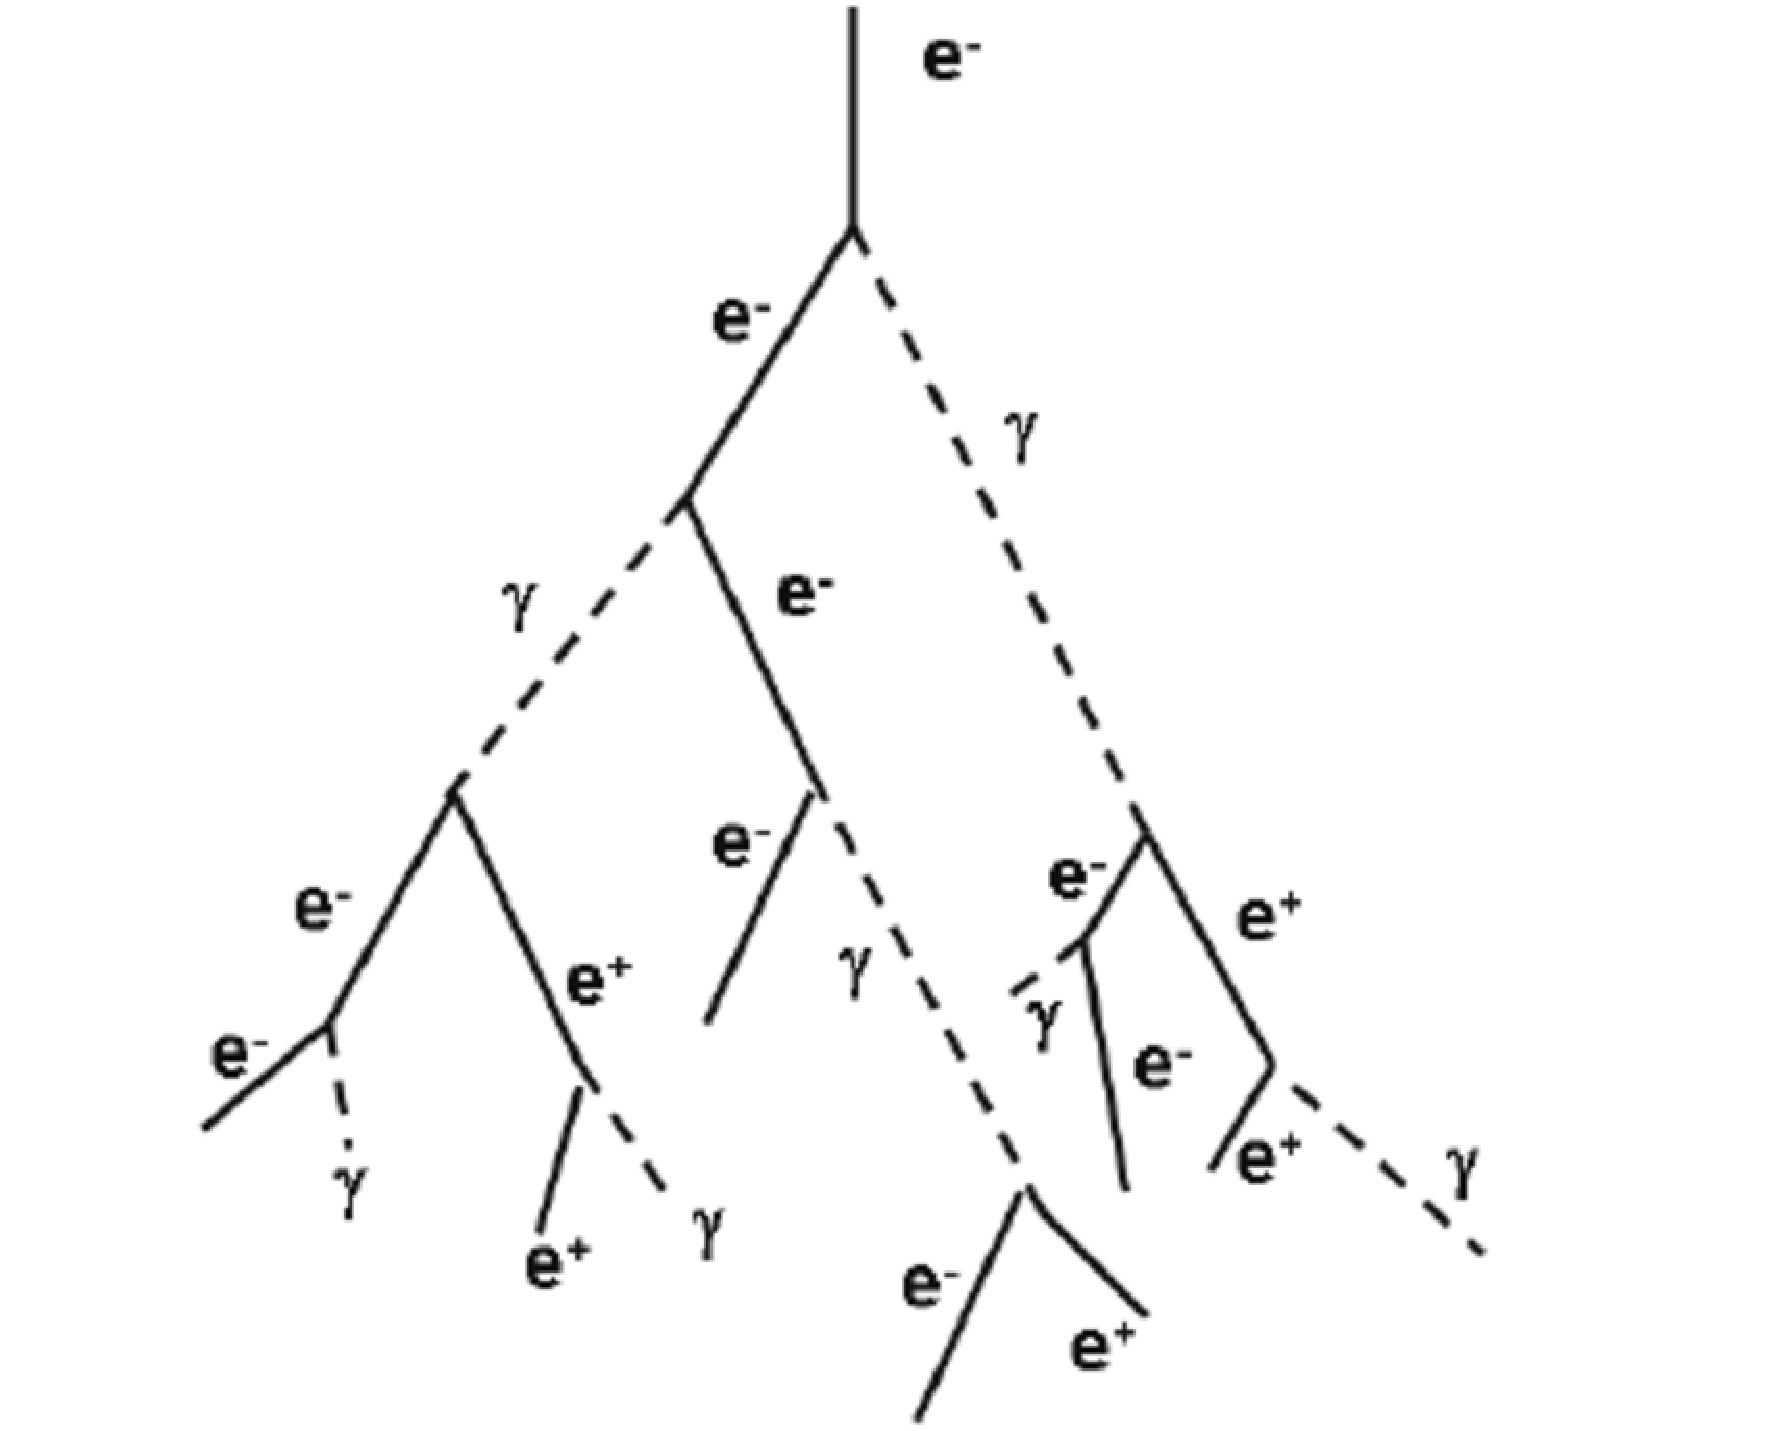
\includegraphics[width=0.4\textwidth]{figures/detector/elec_shower}}
\subfigure{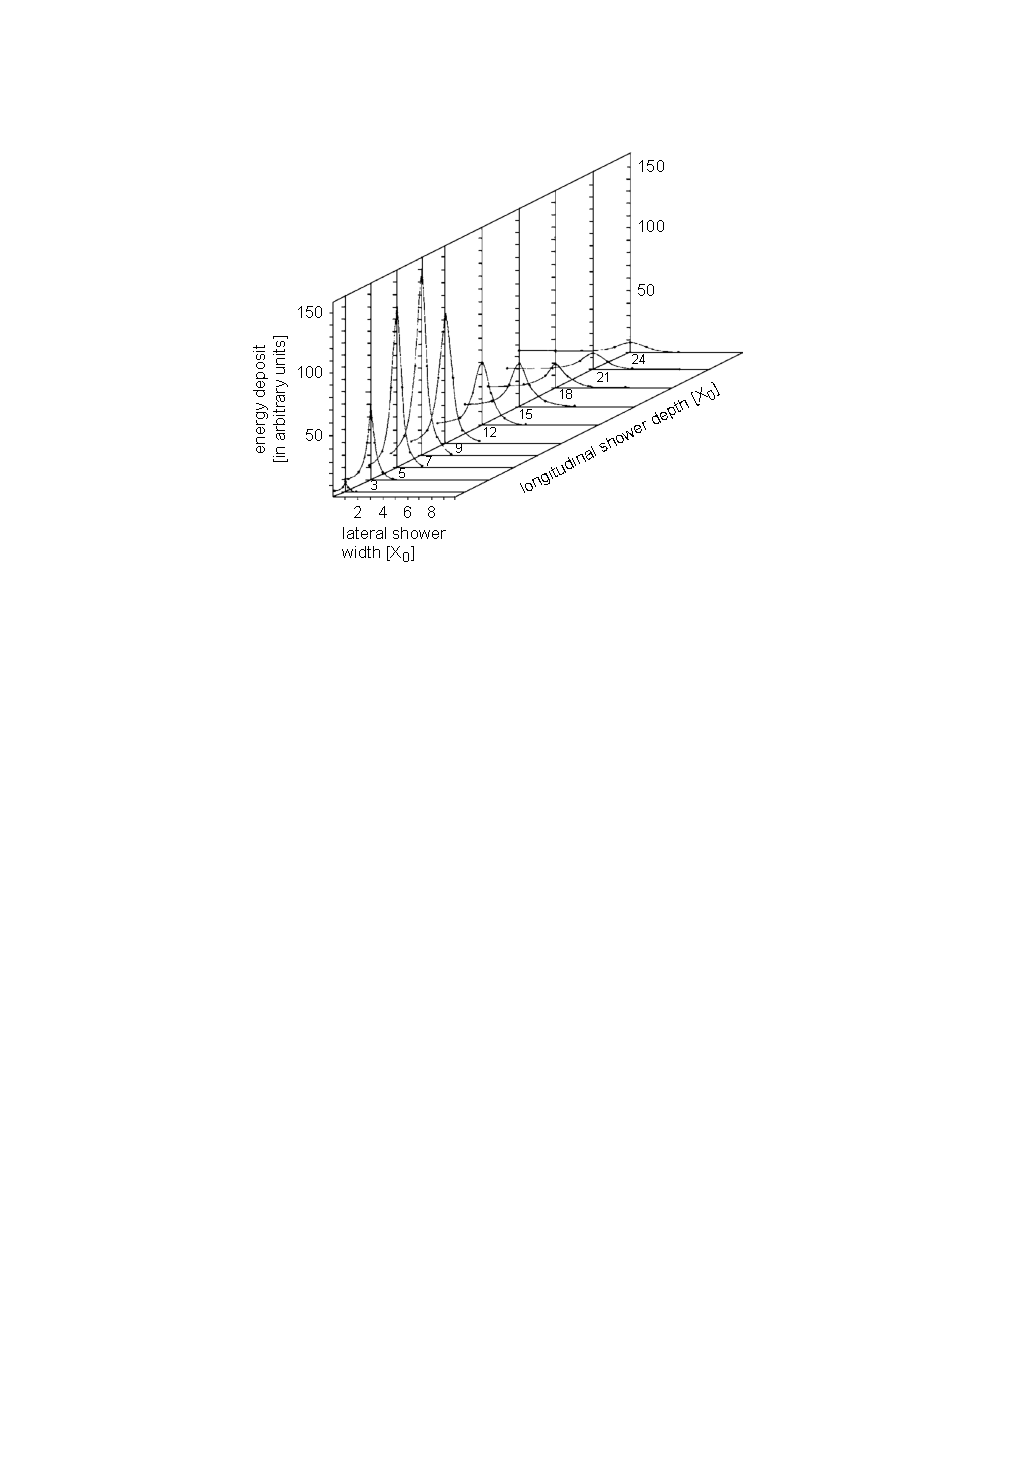
\includegraphics[width=0.57\textwidth]{figures/detector/elec_shower_lateral}}
\caption{(a) Sketch of the evolution of an electromagnetic shower. (b) Lateral and longitudianl evolution of the shower form 6-GeV electons. Figure from Ref. \cite{grupen_shwartz_2008}.}
\label{fig:det:shower_elec}
\end{figure}

\subsubsection{Hadronic Shower}


\begin{figure}[ht]
\centering
\subfigure{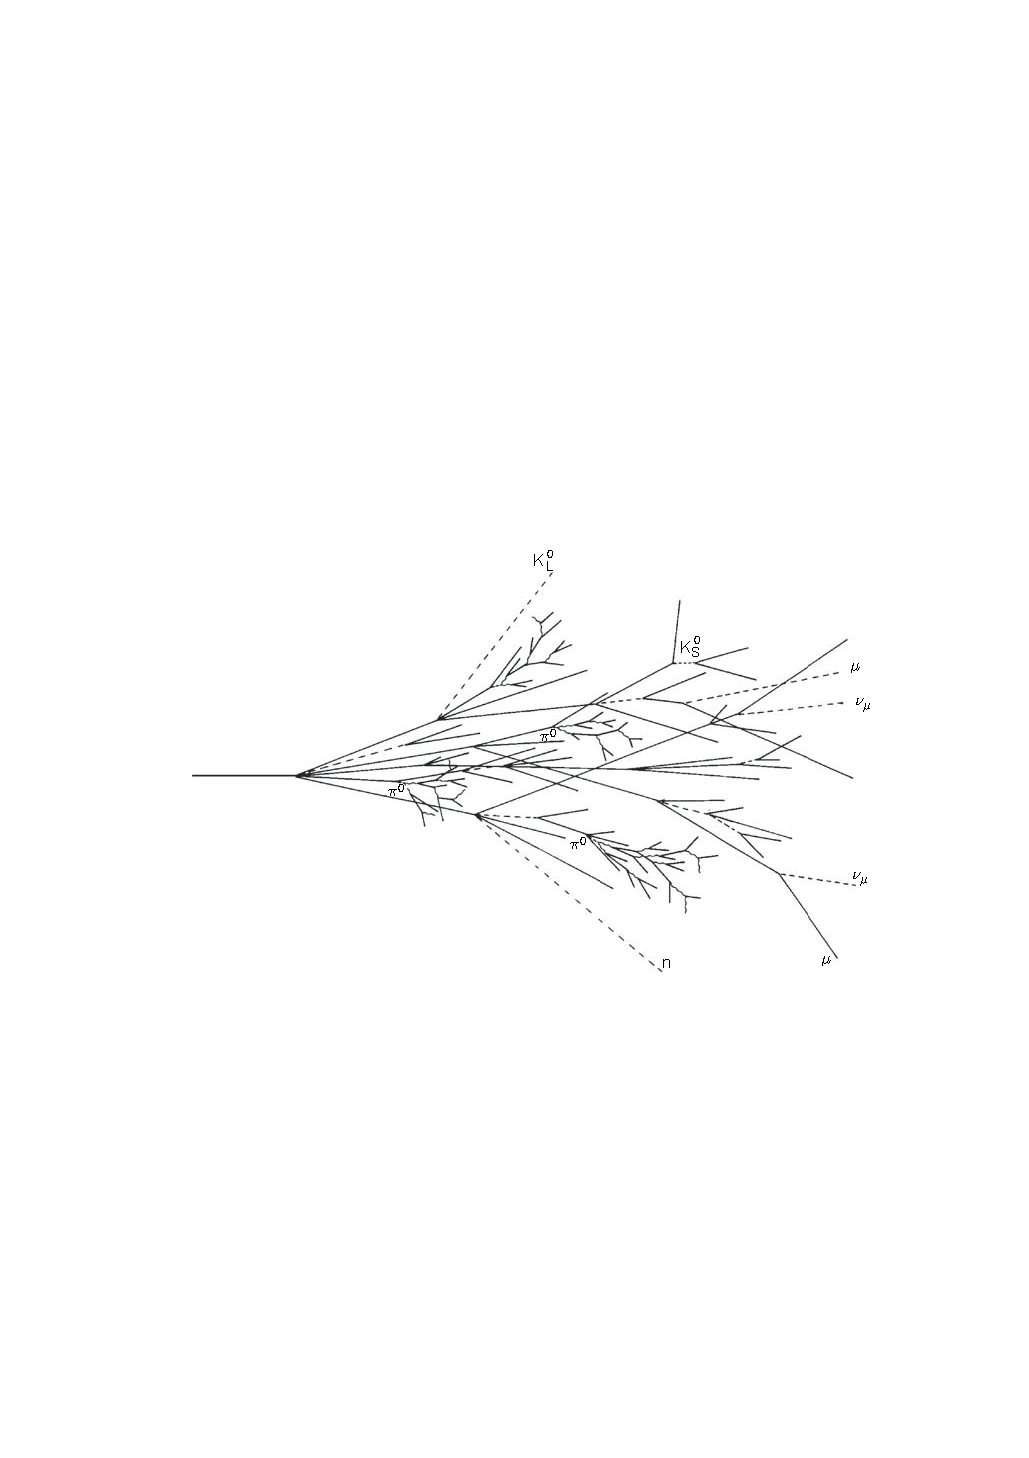
\includegraphics[width=0.48\textwidth]{figures/detector/hadron_shower}}
\subfigure{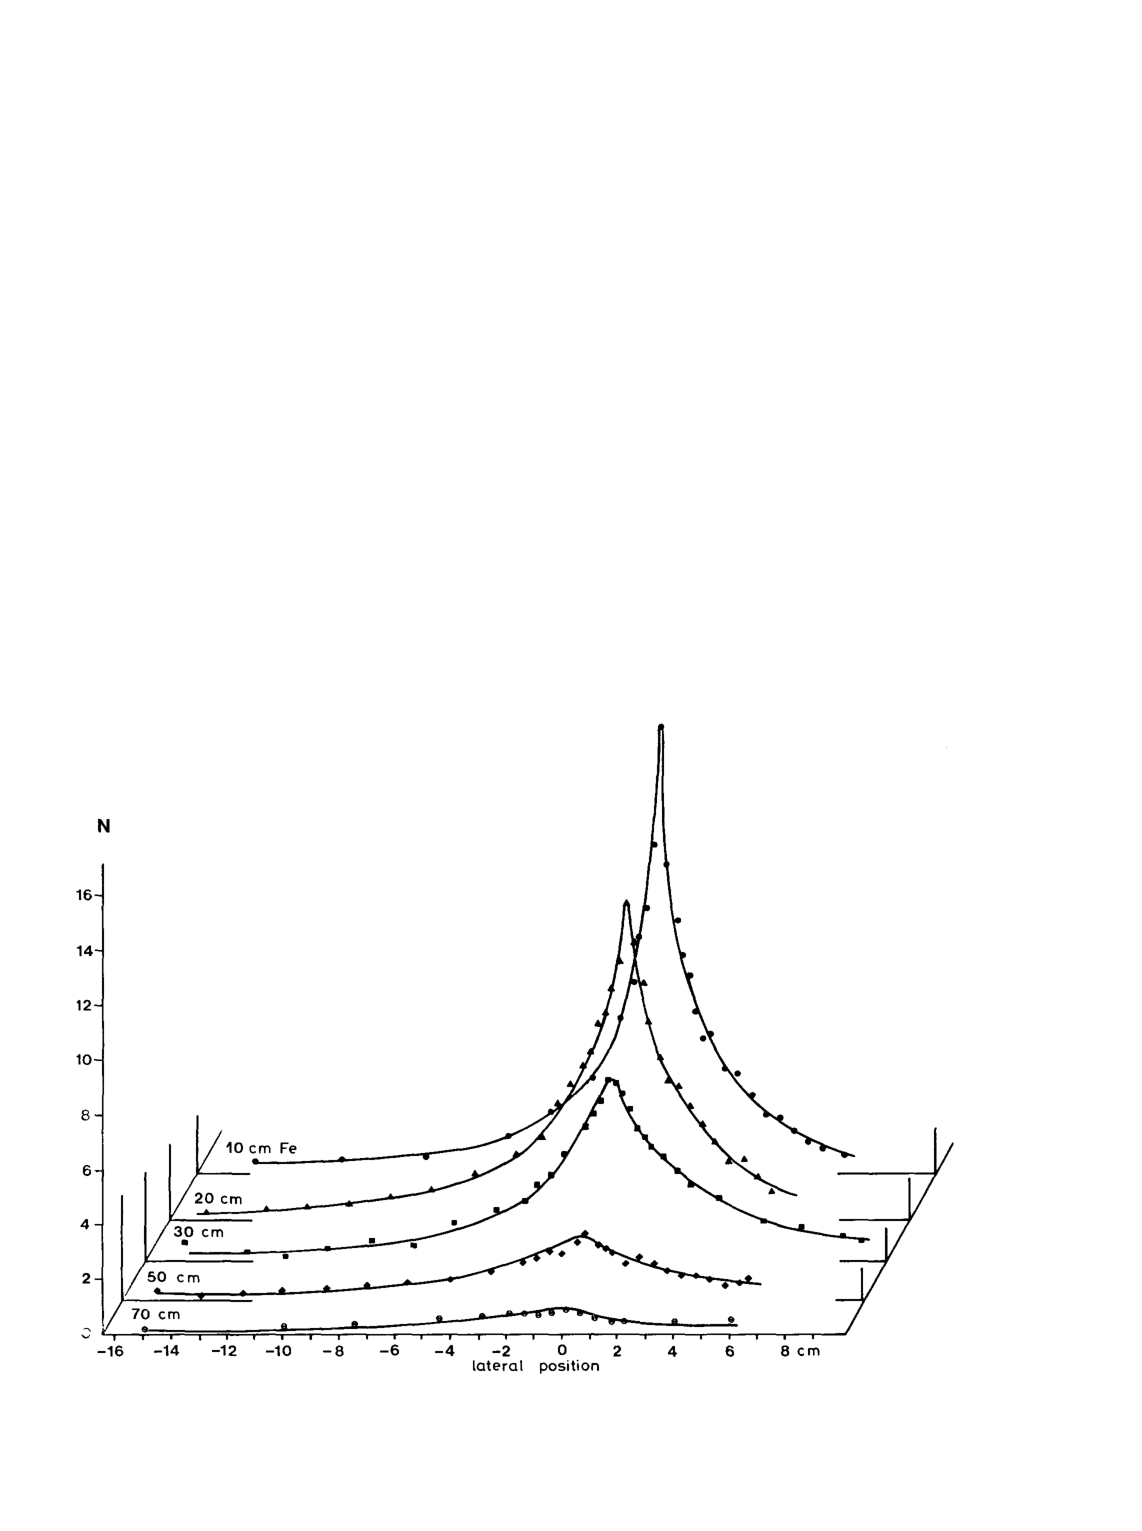
\includegraphics[width=0.48\textwidth]{figures/detector/hadron_shower_lateral}}
\caption{(a) Sketch of the evolution of an hadronic shower. Figure from Ref. \cite{grupen_shwartz_2008}. (b) Lateral energy distribution of shower induced by 10-GeV $\pi^-$, measured at a depth of 10, 20, 30, 50 and 70 cm in Fe. Fig from Ref. \cite{FRIEND1976505}.}
\label{fig:det:shower_had}
\end{figure}

\subsubsection{Types of Calorimeters}
%%%%%%%%%%%%%%%%%% ATLAS

\section{The ATLAS experiment}
\label{sed:cern:atlas}

\gls{atlas} \cite{atlas:atlas}, shown in Fig. \ref{fig:atlas:atlas}, is the largest of the \gls{lhc} detectors, 
measuring 44 meters in length and 25 meters in height, and weighting about 700 tons. 
To be fully functional in the \gls{lhc} environment,  the \gls{atlas} detector needs to be fast in order to resolve the collisions resulting from consecutive bunches (which are interspaced by 25 ns) and radiation resistant. 

\begin{figure}[ht]
\centering
\subfigure{\includegraphics[width=0.85\textwidth]{figures/atlas/atlas}}
\caption{Drawing of the \gls{atlas} detector showing the different subdetectors and
the magnet systems. Figure from Ref. \cite{atlas:atlas}.}
\label{fig:atlas:atlas}
\end{figure}

The \gls{atlas} physics program covers a large variety of topics: 
\begin{itemize}
\item \textit{Standard Model} processes can be measured at the \gls{lhc} at energies never reached before, and being sensitive to them is essential both to provide accurate measurements and to use them as candles to calibrate the detector. 
\item The discovery of the \textit{Higgs boson} was one of the main goals of the \gls{lhc} and, after its observation in 2012, the focus moved onto measuring its properties. 
\item Compared to the Tevatron, the \gls{lhc} is a true \textit{top-quark} factory, 
and the study of the properties of this particle can both probe the \gls{sm} and set limits on \gls{bsm} theories.
\item The \gls{lhc} offers an exciting opportunity to discover \textit{\gls{bsm} physics}, and \gls{atlas} needs to be ready to identify its signs.
\item Despite the ALICE detector is specifically designed to study heavy-ion collisions, \gls{atlas} also carries out a \textit{heavy-ion program}.
\end{itemize}

To cope with the wide range of types and energies (from few GeV to several TeV) of particles that need to be identified, \gls{atlas} relies on a sequence of subdetectors nested in a cylindrical geometry, that follow the general schema discussed in Section \ref{sec:detectors:identification}: close to the \gls{ip} we find the \gls{id}, embedded in a solenoidal magnetic field of 2 T. The following layers are the \gls{ecal} and \gls{hcal}, and the outermost part is occupied by the muon system, where muons are bent by a 4 T toroidal magnetic field. All these components are described in the next sections.

\subsection{Coordinate system}

\gls{atlas} uses a right-handed coordinate system, with its origin at the nominal \gls{ip}. The $z$-axis follows the beam direction, while in the transverse plane the $y$-axis points upward and the $x$-axis toward the \gls{lhc} center. Positive and negative values of the $z$-axis identify respectively the A-side and the C-side of the detector. When spherical coordinates are used, the \textit{azimuthal angle} $\phi$ is defined starting from the $x$-axis, and ranges between $-\pi$ and $\pi$; the \textit{polar angle} $\theta$ is defined starting from the $z$-axis and takes values between $0$ and $\pi$. Often the polar angle is substituted by the \textit{pseudorapidity}: 
 
\begin{equation}
\eta = - \ln\tan\left(\frac{\theta}{2}\right) \; ,
\label{eq:cern:eta}
\end{equation}

\noindent which, in the limit of massless particles, is equivalent to the \textit{rapidity}:

\begin{equation}
y = \frac{1}{2} \ln\left(\frac{E + p_z}{E - p_z}\right) \; ,
\label{eq:cern:y}
\end{equation}

\noindent where $E$ is the energy of the particle and $p_z$ its momentum projected on the $z$-axis. 
The advantage of rapidity and pseudorapidity over the polar angle is that rapidity differences $\Delta y$ are boostinvariant
along the $z$-axis, as well as pseudorapidity differences $\Delta \eta$ for massless particles.
The pseudorapidity is usually preferred to the rapidity as it does not require
knowing the particle’s mass but only its polar position.
The $\eta$-$\phi$ plane is used to define the angular separation of two objects in the detector:

\begin{equation}
\Delta R = \sqrt{ (\Delta \eta)^2 + (\Delta \phi)^2  } \; .
\label{eq:cern:dR}
\end{equation}

Since protons are composite particles, and the hard scattering happens between its constituents, the longitudinal momentum of the partons is unknown. It is therefore useful to define the \textit{transverse momentum} as the projection of the momentum on the ($x$,$y$) plane: 

\begin{equation}
p_T = \sqrt{p_x^2 + p_y^2} \; ,
\label{eq:cern:pt}
\end{equation}

\noindent where $p_{x(y)}$ are the projection of the momentum along the $x$-($y$-)axis.



\subsection{Magnet system}
\label{sec:atlas:magnets}

The two segments of the \gls{atlas} detector that are dedicated to tracking, the \gls{id} and the muon spectrometers, are embedded in two separate magnetic fields. A schematic overview of the \gls{atlas} magnetic system is shown in Fig. \ref{fig:atlas:magnet}.
\label{sec:cern:atlasmagnets}
\begin{figure}[ht]
\centering
\subfigure{\includegraphics[width=0.45\textwidth]{figures/atlas/magnets}}
\caption{Layout of the \gls{atlas} magnet system. Figure from Ref. \cite{Goodson}.}
\label{fig:atlas:magnet}
\end{figure}

As discussed in Section \ref{sec:dec:tracking}, the magnetic field configurations that are more suitable for a detector with cylindrical symmetry are solenoidal and toroidal. The bending of the charged particles in the \gls{atlas} \gls{id} is caused by an axial 2 T solenoidal field, provided by the \textit{central solenoid} \cite{YAMAMOTO200853}. This magnet is 5.8 m long, has an inner diameter of 2.46 m and an outer diameter of 2.56. The wounded coil is made of an Al-stabilised NbTi conductor, and is powered with a 7.73 kA current. 


In the muon system, a solenoid would be disadvantageous in the measurement of forward muons, since the resultant magnetic field would not be perpendicular to the trajectory of those particles. The usage of a toroid to provide the outer magnetic field solves this problem. 
The choice of the “open air” toroid configuration allows a good muon
reconstruction performance without relying on the \gls{id}. 
The toroids allow to efficiently generate the magnetic field over a large volume with a reduced amount
of material. This minimizes the amount of multiple scattering, which represents one
of the factors limiting the muon momentum resolution.
The main drawback of the usage of a toroid is that, in order to obtain the same strength of magnetic field, a toroid needs more current than a solenoid (20.5 kA for 4 T).
The \gls{atlas} toroid system is divided into two subsystems, to allows for an easier design, 
as well as to provide access to the core part of the detector.
The \textit{barrel toroid} \cite{ATLAS:1997ac} provides a peak field of 3.9 T in the cylindrical shell between the calorimeters and the end of the muon spectrometer, and consists of eight coils contained in individual vacuum vessels.  
The \textit{end-cap toroids} \cite{ATLAS:1997ab} provide the magnetic field necessary to bend the muons in the end-cap region of the spectrometer, and each of them consists of eight coils building a single cold mass, originating a peak field of 4.1 T. 



\subsection{Inner detector}
\label{sec:atlas:id}

The main purposes of \gls{atlas} \gls{id} \cite{ATLAS:1997ag,ATLAS:1997af} are to provide a good momentum resolution of the charged particles produced in the collisions and to allow the determination of secondary vertices. The dimensions of the \gls{id} are determined on one side by the 
radius of the beam pipe and on the other side by the beginning of the \gls{ecal}. The total length is 5.4 m, which provides a coverage up to $|\eta|<$2.5.
The \gls{id} is divided into a barrel, whose schema is shown in Fig. \ref{fig:atlas:id}, and two end-cap regions, covering respectively the pseudorapidity regions $|\eta|<1.2$ and $1.2<|\eta|<2.5$. In both, a mixture of gaseous and silicon detectors is used to maximize the performance and reduce the costs. The three components of the \gls{id} are the pixel detector, the semi-conductor tracker, and the transition radiation tracker, discussed in the following paragraphs.

\begin{figure}[ht]
\centering
\subfigure{\includegraphics[width=0.65\textwidth]{figures/atlas/inner_detector}}
\caption{Layout of the \gls{atlas} \gls{id}. Figure from Ref. \cite{Potamianos:2016ptf}.}
\label{fig:atlas:id}
\end{figure}


\subsubsection*{Pixel detector}
\label{sec:atlas:pixel}
The innermost layer of the \gls{id} is the \textit{pixel detector}, divided into barrel and end-cap regions. 
During the Long Shutdown after the \gls{lhc} Run 1, the \gls{id} was subject to important upgrades \cite{Potamianos:2016ptf}. 
The main one is the addition of a fourth pixel layer in the barrel, in addition to the three already existing ones, 
the \gls{ibl} \cite{Capeans:1291633}, that is positioned 3.33 cm away from the \gls{ip}. 
In order to locate a detector so close to the \gls{ip}, the beam pipe had to be replaced with a thinner one. 
The \gls{ibl} is 72.4 cm long along the $z$-direction, and consists of 14 staves that provide full coverage in azimuthal angle. Each stave contains 20 modules, 12 with planar silicon sensors and eight with 3D pixel sensors \cite{1748-0221-7-11-P11010}, and each module has 144$\times$328 pixels with the size of 50$\times$250 $\mu$m$^2$, for a total of over 12 million pixels in the entire \gls{ibl}. The size of the pixels leads to a resolution of 40 and 8 $\mu$m respectively in the longitudinal and transverse direction. 
The three outer pixel layers are located at 5.05, 8.85 and 12.5 cm from the \gls{ip}. 
Each module contains 80 pixels of 50$\times$400 $\mu$m$^2$, leading to a spatial resolution of 115 and 10 $\mu$m respectively in the longitudinal and transverse direction. 
The two end caps, on the two sides of the detector, consist of three wheels each, with a radius of 34 cm and located at 49.5, 58.8 and 65.0 cm from the \gls{ip}. 
To ensure a good performance, the pixel detectors need to be kept at a low and stable temperature, 
between -15$^{\circ}$ C and 5$^{\circ}$ C for the \gls{ibl}, and between -15$^{\circ}$ C and -10$^{\circ}$ C for the other layers.

\subsubsection*{Semi-conductor tracker}
The \gls{atlas} \gls{sct} is composed by 4088 silicon micro-strip modules with binary readout mounted on carbon fibre composite structures, and is organized in four cylinders in the barrel and nine disks in each of the forward regions \cite{Jackson:sct}. The cylinders have  radii of 30.0, 37.3, 44.7 and 52.0 cm and provide a coverage for $|\eta|<1.1-1.4$, while the disks cover the region with $1.1-1.4<|\eta|<2.5$. 
Out of the 4088 \gls{sct} modules, 2112 modules are in the barrel, 
and contain single-sided p-in-n silicon strips, with a pitch of 80 $\mu$m. 
In each module, the strip sensors are positioned back to back with an angle of 40 mrad, to be able to access information on the $z$-coordinate as well. The end-cap modules use strips with width between 56.9 and 94.2 $\mu$m. 
These choices lead to a spatial resolution of 580 $\mu$m in the longitudinal direction and 17 $\mu$m in the transverse one.
Also the \gls{sct} components need to be kept at a low temperature, between -15$^{\circ}$ C and -5$^{\circ}$ C.

\subsubsection*{Transition radiation tracker}

The \gls{trt} is the outermost layer of the \gls{id}. In the barrel it consists of 52544 straw tubes with a length of 1.5 m disposed parallel to the beam direction, while each end-cap contains 122880 straw tubes 0.4 m long disposed perpendicularly to the beam axis. Each tube is 4 mm in diameter, and has in the inside gold plated tungsten wire as anode with a diameter of 31 $\mu$m. The tubes are filled with a mixture of 70\% Xe, 27\% CO$_2$ and 3\% O$_2$; due to a gas leakage, in 2016 part of the \gls{trt} tubes have been filled with a cheaper mixture of 80\% Ar and 20\% CO$_2$. The \gls{trt} has a pseudorapidity coverage up to $|\eta|<2$ and it provides tracking information only in the (r-$\phi$) plane, with a resolution of 130 $\mu$m.


\subsection{Calorimeters}
\label{sec:atlas:calo}

The \gls{atlas} calorimeter system is located outside the \gls{id} and the magnetic field of the solenoid, as shown in Fig. \ref{fig:atlas:calo}. The \gls{ecal} is closer to the \gls{ip}, while the \gls{hcal} is on the outside; both systems have a barrel and an end-cap section. 
The combined thickness of the calorimeter system is about 11 interaction lengths to ensure the longitudinal containment of energetic jets, 
as well as a good reconstruction of the energy imbalance in the event, which is a measure of the energy carried away by neutral weakly-interacting particles. The total pseudorapidity coverage is up to $|\eta|<4.9$. 

\begin{figure}[ht]
\centering
\subfigure{\includegraphics[width=0.75\textwidth]{figures/atlas/calorimeters}}
\caption{Layout of the \gls{atlas} calorimeter system. Figure from Ref. \cite{atlas:atlas}.}
\label{fig:atlas:calo}
\end{figure}

Table \ref{tab:atlas:cal:reso} summarizes the energy resolution of the different subsystems. As expected from the discussion in Section \ref{sec:dec:calo}, the resolution is better for electromagnetic showers than for the hadronic ones. For example, a 1 GeV particle detected in the \gls{ecal} has an energy resolution of about 19\%, while 50\% (100\%) if detected in the \gls{hcal} barrel (end-caps). On the other hand, a 1 TeV particle has an energy resolution of 0.7\% in the \gls{ecal} and 3\% (10\%) in  \gls{hcal} barrel (end-caps), and in this case the resolution is dominated by the constant term, 
related to instrumental effects and to the different response of the detectors to electromagnetic and hadronic showers. 

\begin{table}[ht]
\begin{center}
\begin{tabular}{c c }
\hline
Component & $\sigma_E / E$ \\
\hline 
\hline
\gls{ecal} & 0.1$/\sqrt{E[GeV]}$ $\bigoplus$ 0.17$/E$ $\bigoplus$ 0.007 \\ % chiara: cite LAr TDR
\hline
\gls{hcal} barrel & 0.5$/\sqrt{E[GeV]}$ $\bigoplus$ 0.03 \\
\hline
\gls{hcal} end caps & 1$/\sqrt{E[GeV]}$ $\bigoplus$ 0.1 \\
\hline
\end{tabular}
\end{center}
\caption{Energy resolution of the \gls{atlas} calorimeters.}
\label{tab:atlas:cal:reso}
\end{table}

\begin{figure}[ht]
\centering
\subfigure[]{\includegraphics[width=0.495\textwidth]{figures/atlas/barrel_em.pdf}}
\subfigure[]{\includegraphics[width=0.495\textwidth]{figures/atlas/fisarmonica.jpeg}}
\caption{(a) Schema of a barrel module of the \gls{atlas} \gls{ecal}. Figure from Ref. \cite{atlas:atlas}. (b) Accordion shape of the metal plates of the \gls{ecal}.}
\label{fig:atlas:lar}
\end{figure}

\subsubsection*{Electromagnetic calorimeter}

The \gls{ecal} is a sampling calorimeter with \gls{lar} as active material and \textit{lead plates} as absorber, both in the barrel and in the end caps. The lead plates have a characteristic accordion shape and, in the barrel, are oriented in the radial direction. Before the \gls{ecal}, a presampler provides the information necessary to reconstruct the amount of energy lost in the passive material of the solenoid. The design of a \gls{lar} barrel module is shown in Fig. \ref{fig:atlas:lar}(a), where it is possible to see the segmentation in three layers with decreasing granularity: the first layer is finely segmented in pseudorapidity, with strips of $\Delta\eta \times \Delta\phi = 0.0031 \times 0.098$; the second layer has towers of $\Delta\eta \times \Delta\phi =  0.025 \times 0.025$ to measure the clusters, while the third layer has wider towers of $\Delta\eta \times \Delta\phi =  0.05 \times 0.0245$ to provide an estimate of the energy leaking outside the \gls{ecal}. The \gls{lar} barrel offers pseudorapidity coverage up to $|\eta|<$1.475, and the thickness of the detector varies from 22 $X_0$ at $\eta=0$ to 33 $X_0$ at $|\eta|=1.3$. 
Each of the two end-cap regions consists of two coaxial wheels, of eight modules each, that cover the region $1.375<|\eta|<3.2$, with a thickness varying between 26 and 36 $X_0$ for the inner wheel and between 24 and 38 $X_0$ for the outer wheel. The end-cap modules are divided into two layers, again with decreasing granularity.


\subsubsection*{Hadronic calorimeter}

The hadronic calorimeter is composed of three subsystems with different technologies: the \gls{tilecal} \cite{TileTDR} is a sampling calorimeter with plastic scintillator as active material and steel as absorber, the \textit{hadronic end-cap calorimeter} (HEC) uses copper as absorber and liquid argon as scintillator, while the \textit{forward calorimeter} (FCal) also uses liquid argon in the active layer but has tungsten rods embedded in a copper matrix as absorber. The choice of the materials is driven by the need to have detectors more resistant to radiation in the forward region, where the flux of particles is larger. 

\gls{tilecal} covers the pseudorapidity region with $|\eta|<1.7$, and is divided into a central \gls{lb}, 5.8 m long, and two \glspl{eb}, 2.6 m long; the \gls{tilecal} inner radius is 2.28 m, and the outer radius 4.25 m. Each barrel is divided in 64 modules, disposed on the $\phi$ direction and each having the size of 0.1 radians. Each module is further segmented radially into three layers with thicknesses of about 1.5, 4.1 and 1.8 $\lambda_I$ in the \gls{lb} and 1.5, 2.6 and 3.3 $\lambda_I$ in the \gls{eb}; a schematic of one module is shown in Fig. \ref{fig:atlas:tile}(a). Ionizing particles passing through the plastic scintillator (polystyrene) produce ultra-violet light, which is then collected at the two edges of each tile and converted to the longer wavelength of visible light by wavelength-shifting fibers. The fibers, with a diameter of 1 mm each, transmit the light to the readout \glspl{pmt} located in the grinder.

\begin{figure}[ht]
\centering
\subfigure[]{\includegraphics[width=0.4\textwidth]{figures/atlas/tile.pdf}}
\subfigure[]{\includegraphics[width=0.59\textwidth]{figures/atlas/tile_pic.pdf}}
\caption{(a) Schematic representation of a \gls{tilecal} module and its interface with the optical readout. Figure from Ref. \cite{atlas:atlas}. (b) \gls{tilecal} modules before the installation.}
\label{fig:atlas:tile}
\end{figure}

An approximately projective geometry, shown in Fig. \ref{fig:atlas:tile_cells}, is provided by the grouping of the readout fibers into the \glspl{pmt}: this defines a cell structure, and each cell has dimension $\Delta\eta \times \Delta\phi = $ 0.1 $\times$ 0.1 in the first two layers and $\Delta\eta \times \Delta\phi = $ 0.2 $\times$ 0.1 in the third layer. Special cells cover the gap region between the \gls{lb} and the \gls{eb}: the gap scintillators in the pseudorapidity region $1.0<|\eta|<1.2$ and the crack scintillators in the region $1.2<|\eta|<1.6$, in front of the \gls{lar} end caps.

\begin{figure}[ht]
\centering
\subfigure{\includegraphics[width=1.0\textwidth]{figures/atlas/tile_cells.pdf}}
\caption{Layout of the projective geometry of the \gls{tilecal} cells. Figure from Ref. \cite{atlas:atlas}.}
\label{fig:atlas:tile_cells}
\end{figure}

The HEC shares the same cryogenic system as the \gls{ecal} end caps, and covers the region with $1.5<|\eta|<3.2$. Liquid argon is more resistant to radiation than the plastic scintillator used in \gls{tilecal}, and is therefore the preferred choice in the end-cap region. Each side of the HEC consists of two wheels with outer radius of 2.03 m, and each wheel is composed by 32 identical modules. The electromagnetic signal produced in the \gls{lar} is collected by cathodes on the plates. 

The FCal provides coverage in the forward region with $3.1<|\eta|<4.9$. The FCal modules are located at high pseudorapidity, at a distance of 4.7 m along the $z$-axis from the \gls{ip}.


\subsection{Muon spectrometer}

The \gls{ms} \cite{ATLAS:1997ad}, shown in Fig. \ref{fig:atlas:muon}, is the outer layer of the \gls{atlas} detector, and is located in the magnetic field produced by the 4 T toroidal magnets described in Section \ref{sec:atlas:magnets}. It is designed to provide a \pt measurement with a relative uncertainty of 3\% for muons of intermediate \pt, and to maintain a low uncertainty also at higher \pt (about 10\% for muons with \pt of 1 TeV). It consists of four different muon chambers, two dedicated to the precise measurement of the muon tracks traversing the detector, 
and two providing fast event selection for the trigger system. 

\begin{figure}[ht]
\centering
\subfigure{\includegraphics[width=0.65\textwidth]{figures/atlas/muon}}
\caption{Layout of the \gls{atlas} muon system. Figure from Ref. \cite{atlas:atlas}.}
\label{fig:atlas:muon}
\end{figure}

The two systems dedicated to precision measurement are the \gls{mdt} and the \gls{csc}, both present in barrel and end caps. The \glspl{mdt} are proportional drift chambers covering the region $|\eta|<2.7$; they are made of aluminium tubes with a diameter of 30 mm and a length between 700 and 6300 mm, and a cathode wire made of an alloy of tungsten (97\%) and rhenium (3\%). The filling gas is a mixture of Ar, N$_2$, and CH$_4$ with percentages respectively of 91\%, 4\% and 5\%. The \glspl{csc} are multi-wire proportional chambers that cover the region with $2.0<|\eta|<2.7$, where the shorter drift time of this detector (30 ns compared to the 480 ns of the \glspl{mdt}) allows to better cope with the increase in particle flux in the forward region. The anode wires in the \glspl{csc} are made of the same tungsten-rhenium alloy of the \glspl{mdt} and have a 2.54 mm pitch, which is the same distance separating them from the copper cathode strips, creating a symmetric cell. The gas inside the chamber is a mixture of 30\% Ar, 50\% CO$_2$, and 20\% CF$_4$. The spatial resolution is 40 $\mu$m in the bending plane and 5 mm in the perpendicular plane.

The muon trigger system needs to be able to identify events with energetic muons in a timescale compatible with assigning them to the correct bunch crossing, that are spaced by 25 ns. The two trigger chambers are the \gls{rpc} and the \gls{tgc}. The \glspl{rpc} are arranged in three layers in the barrel region, outside the outermost \gls{mdt} layer. Each narrow chamber consists of two parallel resistive bakelite plates and is filled with a mixture of 94.7\% C$_2$H$_2$F$_4$, 5\% Iso-C$_4$H$_{10}$, and 0.3\% SF$_6$. The signal is readout by metal plates through capacitive coupling, providing a time resolution of 1.5 ns, while the space resolution is about 1 cm. The \gls{rpc} also provides the $\phi$ coordinate for the track, which is not measured by the \glspl{mdt}. The \glspl{tgc} are multi-wire proportional chambers located in the end caps, filled with a mixture of 55\% CO$_2$ and 45\% n-C$_5$H$_{12}$. Contrary to the \glspl{csc}, the \glspl{tgc} are characterized by a distance between the cathode and the anode shorter than the anode pitch. The pseudorapidity coverage is $1.05<|\eta|<2.7$ for tracking and $1.05<|\eta|<2.4$ for triggering; the time response is similar to that of the \glspl{rpc}, while the spatial resolution is better: between 2 and 7 mm. 

\subsection{Luminosity measurement}
\label{sec:lumimeas}

An accurate determination of the luminosity is important both for \gls{sm} measurements, where often the luminosity uncertainty can dominate in some cases, and for \gls{bsm} searches, where a precise background estimate is a key ingredient to be sensitive to a signal. In the \gls{atlas} detector the luminosity measurement is performed with redundancy by multiple luminometers that use different technologies and algorithms, to allow a better determination of the final number and to assign systematic uncertainties. The instantaneous luminosity in Equation \ref{eq:cern:lumi} can also be expressed following the conventions in Ref. \cite{Aaboud:2016hhf} as product of the number of bunch crossings $N_b$ and the average luminosity per bunch cross $<\mathcal{L}_b>$:
\begin{equation}
\mathcal{L} = N_b <\mathcal{L}_b> = N_b \frac{f <\mu>}{\sigma_{\mathrm{inel}} } \; .
\label{eq:atlas:lumi}
\end{equation}

With respect to the nomenclature of Equation \ref{eq:cern:lumi}, $<\mu>$ is the average pileup per bunch crossing and $\sigma_{\mathrm{inel}}$ the inelastic \gls{pp} cross-section. Because of the finite acceptance and efficiency of the detector, what is measured is:
\begin{equation}
\mathcal{L}_b = \frac{f <\mu_\mathrm{vis}>}{\sigma_{\mathrm{vis}} } \; ,
\end{equation}

\noindent where $<\mu_\mathrm{vis}>$ and $\sigma_{\mathrm{vis}}$ are the product of the corresponding quantities in Equation \ref{eq:atlas:lumi} and the acceptance and efficiency of the detector. Out of these two quantities, $<\mu_\mathrm{vis}>$ is directly measurable during the collisions, while $\sigma_{\mathrm{vis}}$ is determined with the \gls{vdm} method \cite{vanderMeer:296752}, carried out in the dedicated \gls{vdm} runs. These are special runs with low bunch intensity and number of bunches, where a variation (scan) of the overlap of the two beams in the $x$- and $y$-direction is performed; the beam parameters and the peak of visible interaction rate per bunch crossing during the scan can be used to determine the visible cross-section and therefore calibrate each subsystem. 

We can express the luminosity per bunch cross as:
\begin{equation}
\mathcal{L}_b = n_1 n_2 f \int \rho_1(x,y) \rho_2(x,y) \, dx \, dy \; ,
\label{eq:lumi_vdm1}
\end{equation}

\noindent where $\rho_1(x,y)$ and $\rho_2(x,y)$ are the particle densities in the two colliding bunches at the \gls{ip}. 
Under the assumption that these densities can be factorized into the horizontal and vertical components, we can write Equation \ref{eq:lumi_vdm1} as:
\begin{equation}
\mathcal{L}_b = n_1 n_2 f  \Omega_x(\rho_1(x), \rho_2(x)) \Omega_y(\rho_1(y), \rho_2(y))  \; ,
\label{eq:lumi_vdm1}
\end{equation}

\noindent where $\Omega_{x/y}$ defines the beam overlap in the $x$/$y$ direction.

The relevant quantity in physics analyses is the integrated luminosity over a defined period of time. The basic time unit over which the integrated luminosity is computed and stored is the \gls{lub}, whose duration is defined by the \gls{atlas} trigger system and is typically about one minute. The data contained in each \gls{lub} is collected with the same detector conditions, and the integrated luminosity is computed as the average instantaneous luminosity multiplied by the \gls{lub} time duration.

\gls{atlas} has two primary specifically-designed luminometers, LUCID-2 (\textit{LUminosity measurements using Cherenkov Integrating Detector}) and BCM (\textit{Beam Conditions Monitor}), whose results are compared with the one obtained by other \gls{atlas} subsystems that measure luminosity through quantities that are sensitive to it, such as the number of tracks or the flow of particles.

\subsubsection*{Bunch-by-bunch luminometers}

The two dedicated luminometers are able to provide information for individual bunch crossings, each labeled by a \gls{bcid}.

BCM consists of four $8 \times 8$ mm$^2$ diamond sensors, located at $z= \pm 184$ m from the \gls{ip} and disposed in a cross shape around the beam pipe, at $|\eta| = 4.2$. Beside luminosity measurements, BCM is also used to recognize beam losses so that the beam can be dumped before damaging the silicon detectors. 

LUCID is located 17 m from the \gls{ip}, at $5.6 < |\eta| < 6.0$, and consists on each side of 16 Cherenkov detectors built by aluminum tubes with a diameter of 10 mm. Cherenkov radiation is produced in the passage of particles through the quartz windows of the \glspl{pmt}. A signal over threshold produces a hit for that bunch crossing.

%\begin{figure}[ht]
%\centering
%\subfigure{\includegraphics[width=0.75\textwidth]{figures/atlas/forward}}
%\caption{Forward detectors in \gls{atlas}.}
%\label{fig:atlas:forward}
%\end{figure}

\subsubsection*{Tracker-based algorithms}

The \gls{id}, described in Sec. \ref{sec:atlas:id}, records the passage of charged particles as tracks. The number of such charged tracks in each bunch crossing is proportional to the luminosity, and can be used as $<\mu_\mathrm{vis}>$ if averaged over a \gls{lub}. 
During collisions partial data, selected with a random trigger that has the same probability of firing for each colliding bunch, are recorded in a dedicated stream. Because of the high number of colliding bunches, to achieve enough statistical precision the luminosity is provided as integrated over the \gls{lub}; instead, during \gls{vdm} scans, bunch-by-bunch luminosity can be provided. 
% chiara: indicate which track types have been used in 2015-2016 and which in 2017
The reconstruction of the tracks used in this process is described in Sec. \ref{sec:reco:tracks}.

\subsubsection*{Bunch-integrating devices}

The long-term stability of the luminosity measurement provided by BCM, LUCID and the track system is checked with devices that are sensitive to the flux of particles through the detector. This technique only allows to measure the instantaneous luminosity integrated over a time of a few seconds, and not bunch-by-bunch.

A subdetector capable of providing such measurement is \gls{tilecal}, described in Sec. \ref{sec:atlas:calo}. The current generated by the \glspl{pmt} is proportional to the total number of particles; this current is not read through the digital readout system, but through an integrator system sensitive to currents between 0.01 nA and 1.2 $\mu$A over a time window of 10-20 ms. The current induced in different cells varies largely with the cell position: the ones that receive a larger amount of particles are the ones around $|\eta|=1.25$ and in the inner part of the detector (as the hadronic shower is stopped while it passes through the calorimeter). The \gls{tilecal} luminosity measurement is not calibrated during \gls{vdm} scans, but is instead equalized to LUCID or the track measurement for one specific run, and the calibration constant between current and luminosity allows to measure the luminosity also in different runs. More details on the \gls{tilecal} luminosity measurement are given in 
Appendix \ref{app:pmt}. 

Additional systems used in the luminosity determination are the \gls{lar}-based calorimeters in the end caps, the electromagnetic one and the FCal. In both systems the high-voltage (HV) system maintains a constant voltage by supplying a continuous injection of current that counterbalances the voltage drop caused by the flux of particles in a certain sector. The measurement of this current provides a luminosity measurement. Also \gls{lar} systems are not calibrated during the \gls{vdm} scan, but each HV run is calibrated to the baseline luminosity algorithm over a physics run.  


\subsection{Trigger system}
\label{sec:cern:trigger}

With the nominal bunch spacing of 25 ns, the \gls{lhc} produces collisions at a frequency of 40 MHz. This exceeds by several orders of magnitude the current capability to write events to disk; therefore the \gls{atlas} \gls{tdaq} system selects and records the events that are considered interesting for analyses. The \gls{tdaq} system has been updated between Run 1 and Run 2 \cite{Aaboud:2016leb} and it currently consists of a  hardware \gls{lone} trigger and a single software-based \gls{hlt}. A schematic view of the Run 2 \gls{atlas} \gls{tdaq} system is shown in Fig. \ref{fig:atlas:trig}. \gls{lone} is the first step in the chain, and reduces the output rate from 40 MHz to about 100 kHz. It uses reduced-granularity information from the calorimeter systems and from the muon \gls{rpc} and TGS to select events with interesting objects and saves the information about the \gls{roi}. \gls{lone} has a latency time of 2.5 $\mu$s; this corresponds to about 100 collisions, whose information has to be temporarily stored in buffers before the \gls{lone} \gls{ctp} finalizes a decision based on the inputs from the \gls{lonecalo}, \gls{lonemuo} and the \gls{lonetopo}. 

During Run 1 the \gls{hlt} consisted of two separate levels that in Run 2 have been merged to have a simpler setup and better resource sharing. The \gls{hlt} uses information with finer granularity from the calorimeter systems, precision tracking from the muon spectrometer and tracking information from the \gls{id}, not available for \gls{lone}. The \gls{hlt} reduces further the event rate to about 1 kHz, and has a processing time of about 0.2 s per each event. 

A \textit{trigger chain} is a set of selections that characterize a certain trigger object, and the list of all available trigger chains defines the \textit{trigger menu}; some of the items on the menu are \textit{unprescaled}, which means all the events firing that trigger are stored, while others are associated to a \textit{prescale constant} P such that only a fraction $\frac{1}{P}$ of the events firing the trigger are stored.

\begin{figure}[ht]
\centering
\subfigure[]{\includegraphics[width=0.9\textwidth]{figures/atlas/tdaq-run2-schematic}}
\caption{Schematic view of the Run 2 \gls{atlas} \gls{tdaq} system. Figure from Ref. \cite{Aaboud:2016leb}.}
\label{fig:atlas:trig}
\end{figure}


\subsection{ATLAS operation}

\gls{atlas} has been successfully recording the collision data delivered by the \gls{lhc} in Run 1 and Run 2. Figure \ref{fig:atlas:lumi1} shows the cumulative luminosity delivered by the \gls{lhc} between the declaration of stable beams and the request to put the detector in standby for beam dump  as well as the luminosity recorded by \gls{atlas} in 2015 and 2016, which is the dataset used in the analyses described in this thesis. The difference between the two derives from inefficiencies of the data acquisition system and from the "warm start" procedure: the high voltage of the tracking devices and the preamplifiers of the pixel detector are turned on after the start of stable beams \cite{LumiTwiki}.

\begin{figure}[ht]
\centering
\subfigure[]{\includegraphics[width=0.48\textwidth]{figures/atlas/lumi/lumi_2015}\label{fig:atlas:lumi1:a}}
\subfigure[]{\includegraphics[width=0.48\textwidth]{figures/atlas/lumi/lumi_2016}\label{fig:atlas:lumi1:b}}\\
\subfigure[]{\includegraphics[width=0.48\textwidth]{figures/atlas/lumi/lumi_2017}\label{fig:atlas:lumi1:c}}
\subfigure[]{\includegraphics[width=0.48\textwidth]{figures/atlas/lumi/intlumivstimeRun2DQ}\label{fig:atlas:lumi1:d}}
\caption{Cumulative luminosity versus time delivered to (green) and recorded by \gls{atlas} (yellow) during stable beams for pp collisions at $\sqrt{s}=13$ TeV in \subref{fig:atlas:lumi1:a} 2015, \subref{fig:atlas:lumi1:b} 2016, 
and \subref{fig:atlas:lumi1:c} 2017. \subref{fig:atlas:lumi1:d} Cumulative luminosity versus time in 2015-2017 certified to be good quality data (blue). Figure from Ref. \cite{LumiTwiki}.}
\label{fig:atlas:lumi1}
\end{figure}

At the time of this writing, the 2017 dataset has been collected but not yet analyzed. The delivered and recorded luminosity for 2017 is shown in Fig. \ref{fig:atlas:lumi1:c}. Not all the recorded luminosity can be used for physics analyses, as most of these require a good state of all the detector subsystems. This is checked for each luminosity block; the ones with poor detector conditions are disregarded, while the ones that pass this criteria form the \gls{grl}, which imposes requirements on the quality of the beams and of the detector. Figure \ref{fig:atlas:lumi1:d} shows the total cumulative luminosity for the 2015-2017 period, highlighting the portion that enters the \gls{grl}. 




%----------------------------------------------------------------------------------------
%	THESIS CONTENT - APPENDICES
%----------------------------------------------------------------------------------------

\appendix % Cue to tell LaTeX that the following "chapters" are Appendices

% Include the appendices of the thesis as separate files from the Appendices folder
% Uncomment the lines as you write the Appendices

\include{Appendices/test_appendix}

%----------------------------------------------------------------------------------------
%	LIST
%----------------------------------------------------------------------------------------


\listoffigures % Prints the list of figures
\listoftables % Prints the list of tables


%----------------------------------------------------------------------------------------
%	BIBLIOGRAPHY
%----------------------------------------------------------------------------------------

\printbibliography[heading=bibintoc]

%----------------------------------------------------------------------------------------

\end{document}  
